%\RequirePackage{atbegshi}
\documentclass[10pt]{beamer}

\usetheme{default}
\usepackage{amssymb}
\usepackage{biblatex}
%\usepackage[cmex10]{amsmath}
\usepackage{stmaryrd,epsfig}
\usepackage[english]{babel}
\usepackage{tikz,pgf,pgfplots}
\pgfplotsset{compat=newest}
\usepgflibrary{shapes}
\usetikzlibrary{%
  arrows,%
  decorations,%decorations
  shapes.misc,% wg. rounded rectangle
  shapes.arrows,%
  shapes.callouts, %
  shapes,%
  chains,%
  matrix,%
  positioning,% wg. " of "
  patterns,% slanted lines fill
  scopes,patterns,calc,
decorations.markings,
decorations.pathmorphing
}

%\setbeamertemplate{blocks}[rounded][shadow=true]

% Radius of regular polygons
\newdimen\R
\R=0.8cm

\definecolor{tutorial}{RGB}{50,93,61}


\title{Recent Advances in Communication Schemes for Massive Uncoordinated and Unsourced Multiple Access}
\author{J.-F.~Chamberland, Krishna R. Narayanan A.~Vem, A.~Taghavi}
\institute{Electrical and Computer Engineering \\ Texas A\&M University}
\date{Indian Institute of Science, Bengaluru \\ July 7, 2017}

%\setbeamertemplate{footline}[page number]
\setbeamertemplate{navigation symbols}{\textcolor{black}{\insertframenumber / \inserttotalframenumber}}

\begin{document}

\begin{frame}
  \titlepage

\footnotetext[1]{\scriptsize This material is based upon work supported by NSF under Grant No.~1619085.}
\end{frame}


\begin{frame}
\frametitle{\textcolor{black}{Internet of Things \& Anticipated Device Growth}}
\begin{center}
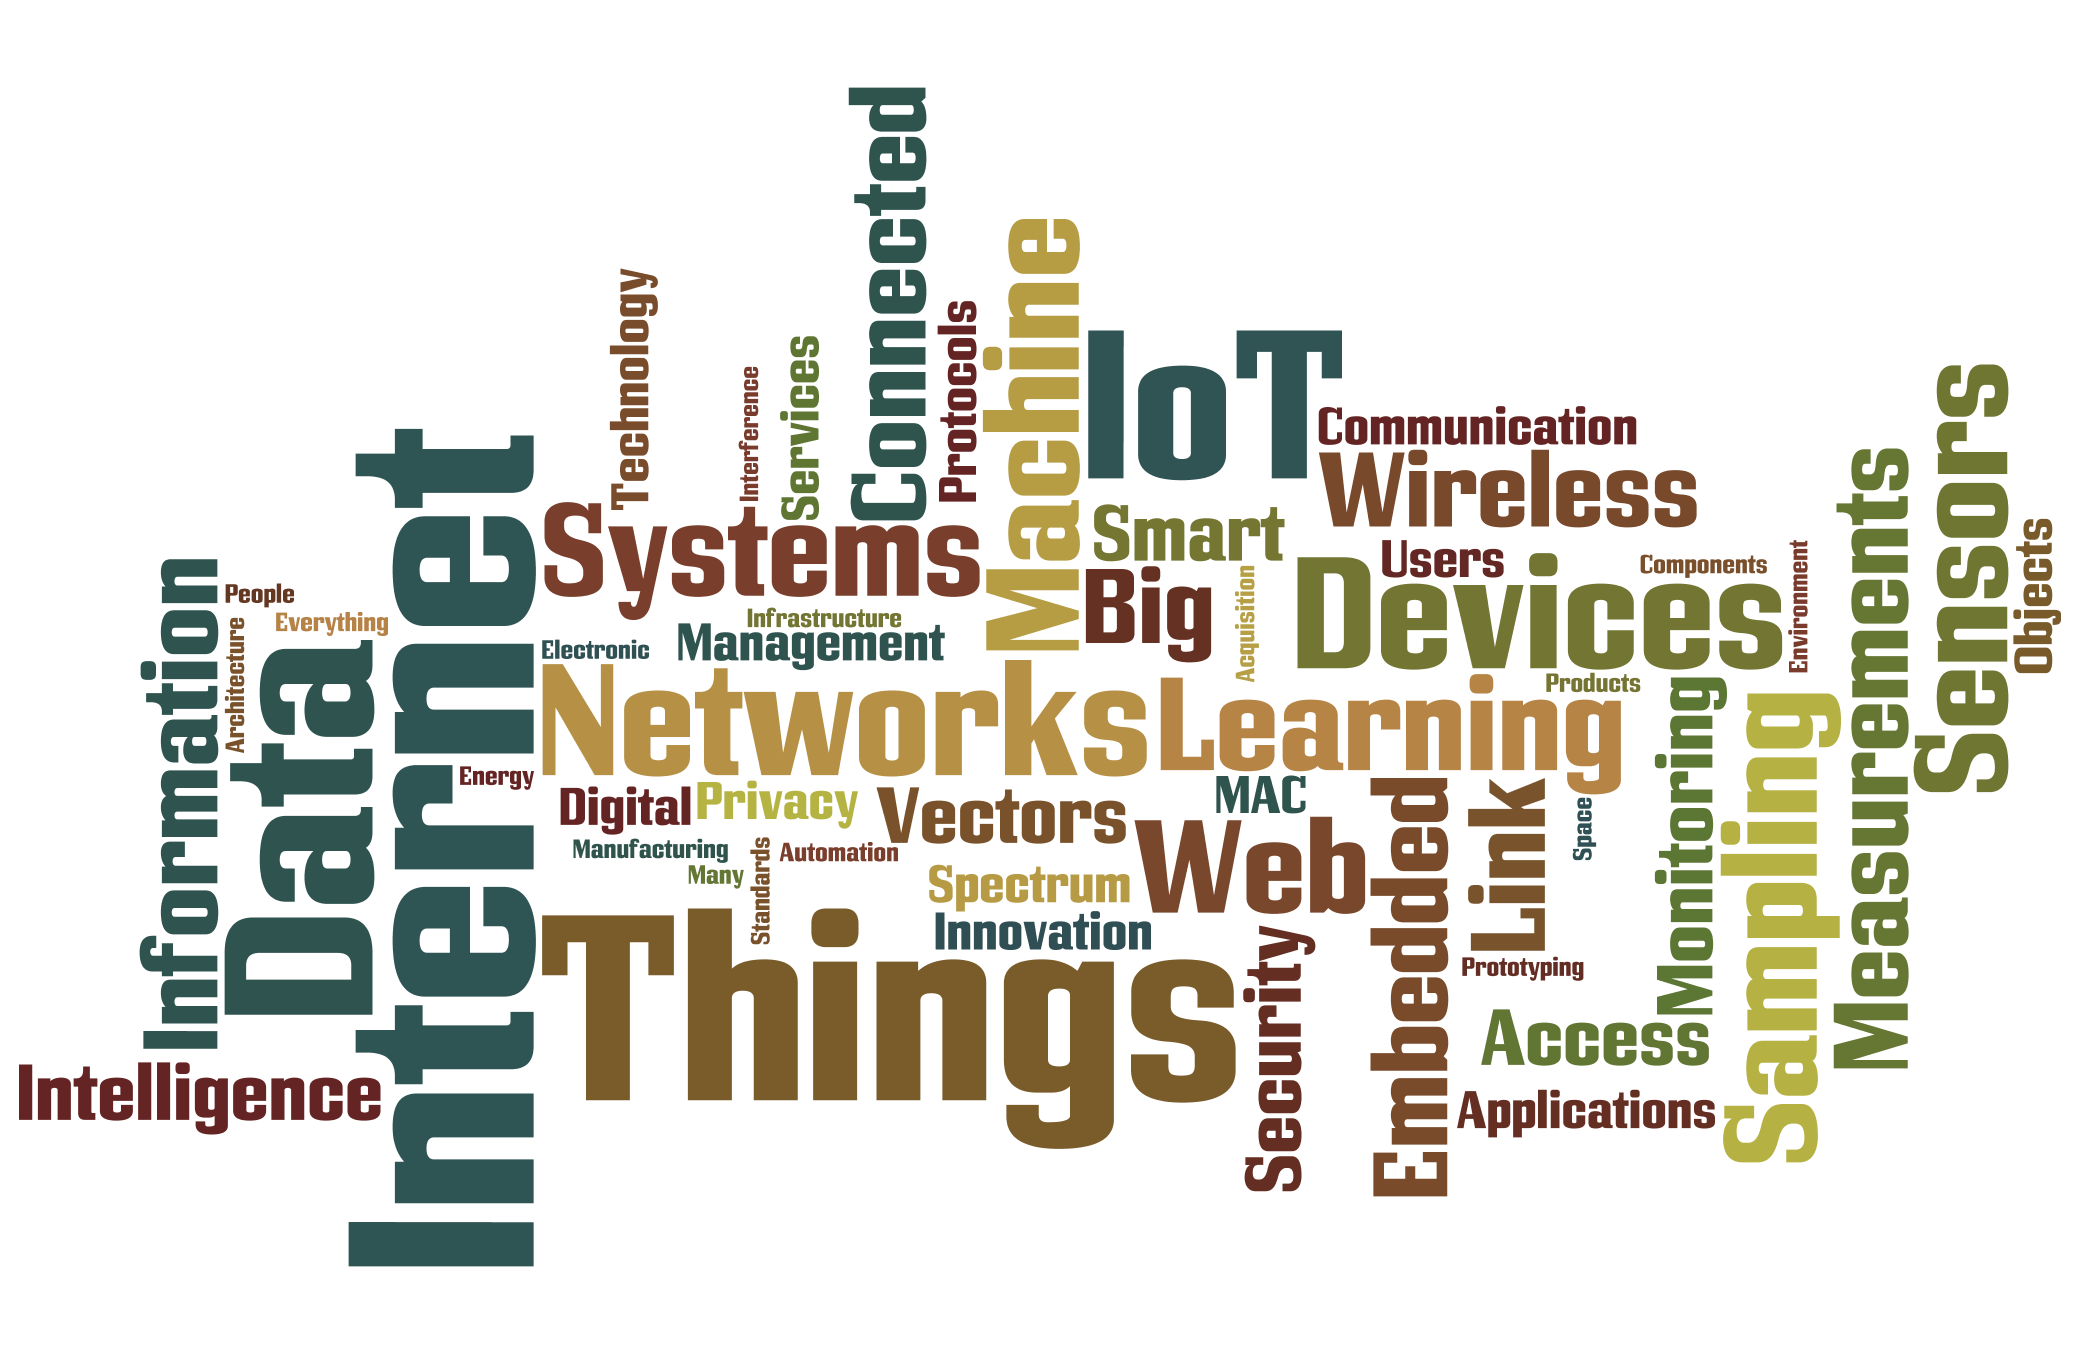
\includegraphics[width=1.0\textwidth]{Figures/Wordle.png}
\end{center}
\end{frame}


\begin{frame}
\frametitle{Motivation for Massive Multiple Access}
\begin{itemize}
\item Current: A few devices with sustained connections
\item 5G: Not just \emph{4G but faster}; includes IoT and M2M communication
\item Future: \textbf{Many uncoordinated} devices with \textbf{sporadic transmissions}
\end{itemize}
\begin{center}
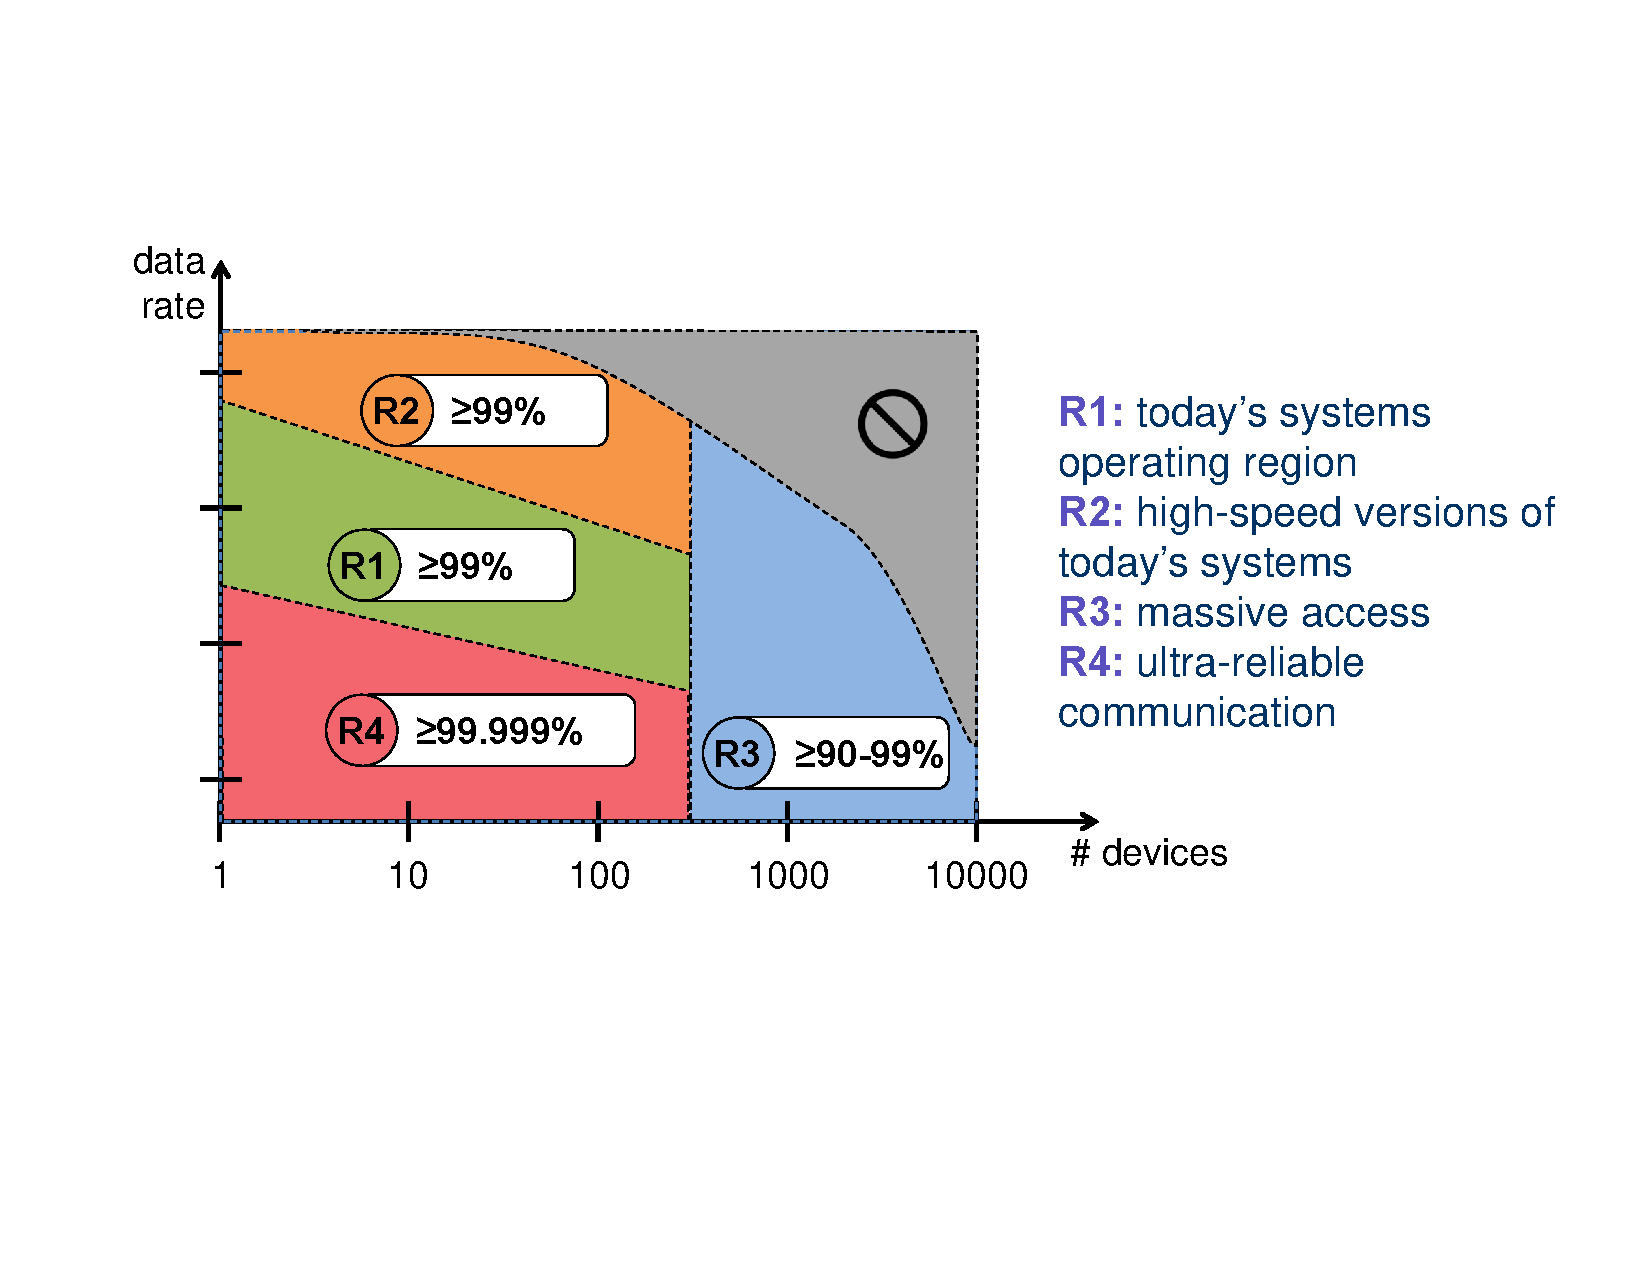
\includegraphics[width=0.9\textwidth]{Figures/5Gchanginglandscape.pdf}
\end{center}
\end{frame}



\begin{frame}
\frametitle{An Evolving Wireless Landscape}
\begin{columns}
\column{.35\textwidth}
  \begin{center}
  \scalebox{0.6}{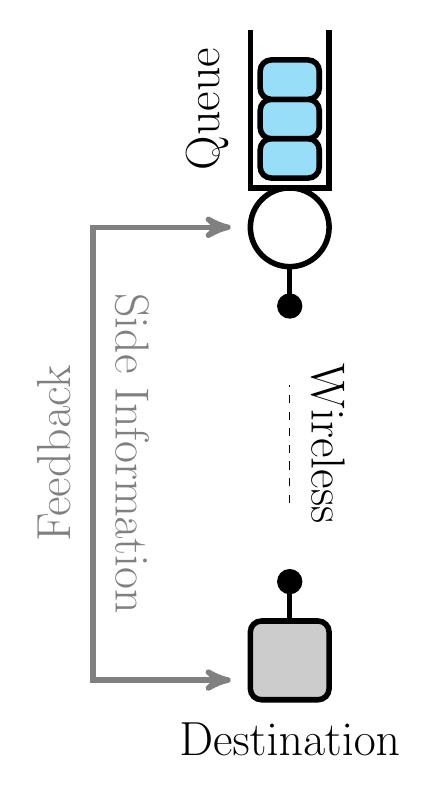
\begin{tikzpicture}
[draw=black, line width=2pt, >=stealth',
queue/.style={circle, draw, inner sep=0pt, minimum size=10mm}]

\draw[fill=cyan!40, rounded corners] (2.125,6.125) rectangle (2.875,6.625);
\draw[fill=cyan!40, rounded corners] (2.125,6.625) rectangle (2.875,7.125);
\draw[fill=cyan!40, rounded corners] (2.125,7.125) rectangle (2.875,7.625);
\draw (2,8) -- (2,6) -- (3,6) -- (3,8);
\node[anchor=south,rotate=90] (queuelength) at (1.875,7) {\LARGE Queue};
\node[queue] (queue0) at (2.5,5.5) {};

\draw[fill=black!20, rounded corners] (2,-0.5) rectangle (3,0.5);
\node (destination) at (2.5,-1) {\LARGE Destination};

\draw (queue0.south) -- (2.5,4.5);
\draw[fill] (2.5,4.5) circle (0.125);
\draw[dashed, line width=0.5pt] (2.5,2) -- (2.5,3.5);
\node[anchor=south,rotate=-90] (wireless) at (2.625,2.75) {\LARGE Wireless};
\draw[fill] (2.5,1) circle (0.125);
\draw (2.5,0.5) -- (2.5,1);


\draw[<->, draw=gray] (1.75,-0.25) -- (0,-0.25) -- (0,5.5) -- (1.75,5.5);
\node[rotate=90] (feedback) at (-0.5,2.625) {\color{gray}{\LARGE Feedback}};
\node[rotate=-90] (sideinfo) at (0.5,2.625) {\color{gray}{\LARGE Side Information}};
\end{tikzpicture}

}
  \end{center}
\column{.6\textwidth}
  \begin{block}{Conventional Systems}
  \begin{itemize}
  \item Human operators, sustained connections
  \item Scheduling decisions based on channel quality \& queue length
  \item Acquisition of side information amortized over long connections
  \end{itemize}
  \end{block}
  \begin{block}{Envisioned IoT Environments}
  \begin{itemize}
  \item Machine-to-machine communications
  \item Sporadic single transmissions from large number of devices
  \item Minute payloads
  \end{itemize}
  \end{block}
\end{columns}
\end{frame}


\begin{frame}
\frametitle{The Cost of Acquiring Side Information}
\begin{center}
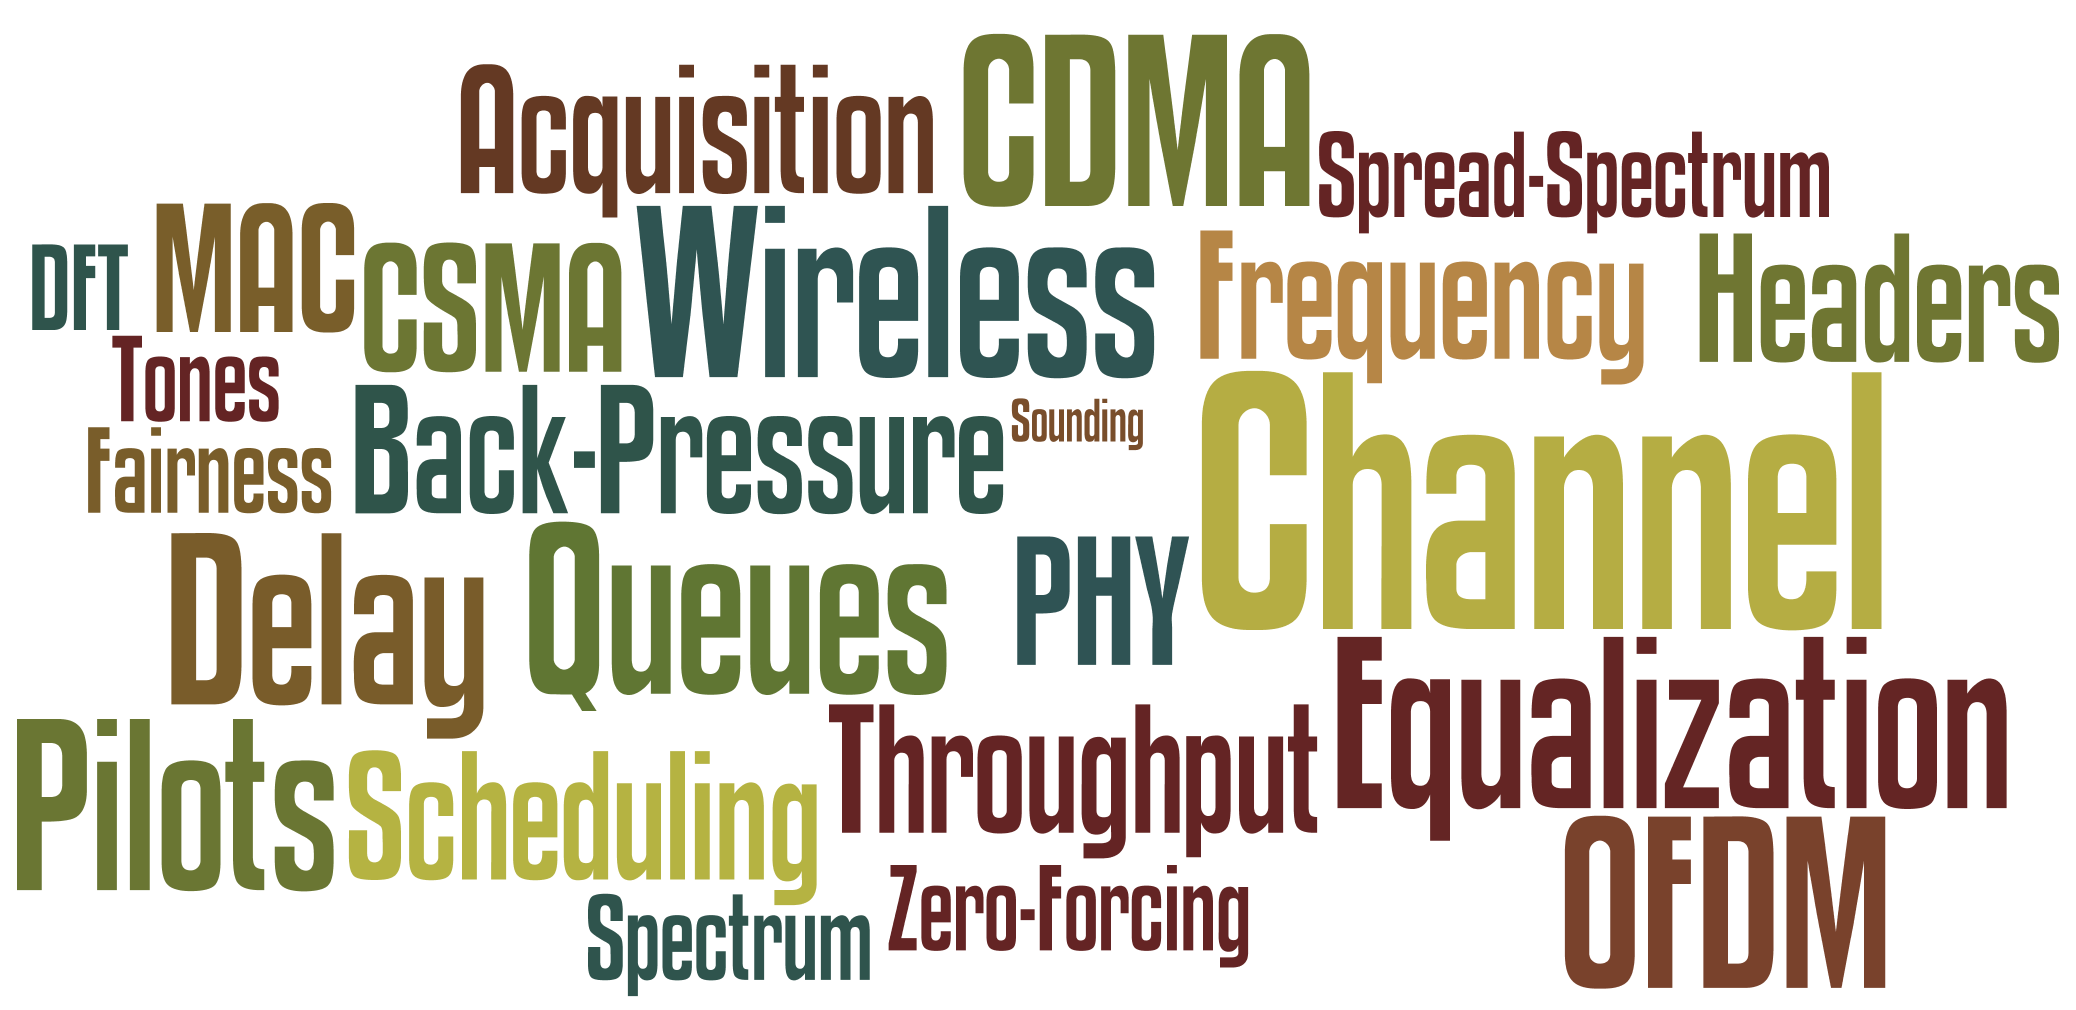
\includegraphics[width=0.7\textwidth]{Figures/SideInfo2.png}
\end{center}
\vfill
\begin{columns}
\column{.45\textwidth}
  \begin{center}
  \scalebox{0.45}{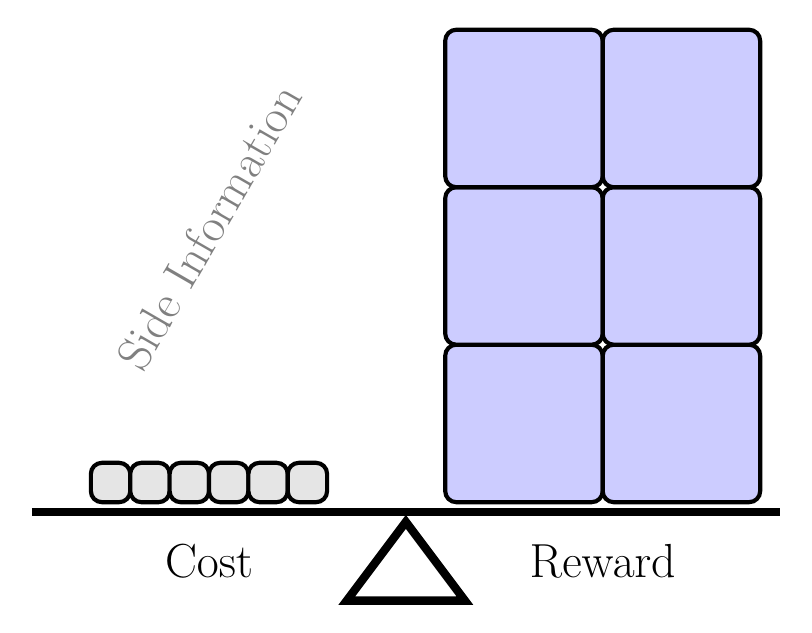
\begin{tikzpicture}
[draw=black, line width=1.5pt, >=stealth',
entry2/.style={rectangle, rounded corners, draw, fill=blue!20, inner sep=0pt, minimum size=20mm},
entry/.style={rectangle, rounded corners, draw, fill=gray!20, inner sep=0pt, minimum size=5mm}]

\node[entry] (r10) at (0.5,0) {};
\node[entry] (r20) at (1,0) {};
\node[entry] (r30) at (1.5,0) {};
\node[entry] (r40) at (2,0) {};
\node[entry] (r50) at (2.5,0) {};
\node[entry] (r60) at (3,0) {};

\node[entry2] (m00) at (5.75,0.75) {};
\node[entry2] (m01) at (5.75,2.75) {};
\node[entry2] (m02) at (5.75,4.75) {};
\node[entry2] (m00) at (7.75,0.75) {};
\node[entry2] (m11) at (7.75,2.75) {};
\node[entry2] (m12) at (7.75,4.75) {};

\draw[line width=3pt] (-0.5,-0.375) -- (9,-0.375);
\draw[line width=3pt] (3.5,-1.5) -- (4.25,-0.5) -- (5,-1.5) -- (3.5,-1.5) -- (4.25,-0.5);

\node (reward) at (1.75,-1) {\LARGE Cost};
\node (cost) at (6.75,-1) {\LARGE Reward};
\node[rotate=60] (info) at (1.75,3.25) {\LARGE \textcolor{gray}{Side Information}};
\end{tikzpicture}
}
  \end{center}
\column{.45\textwidth}
  \begin{center}
  \scalebox{0.45}{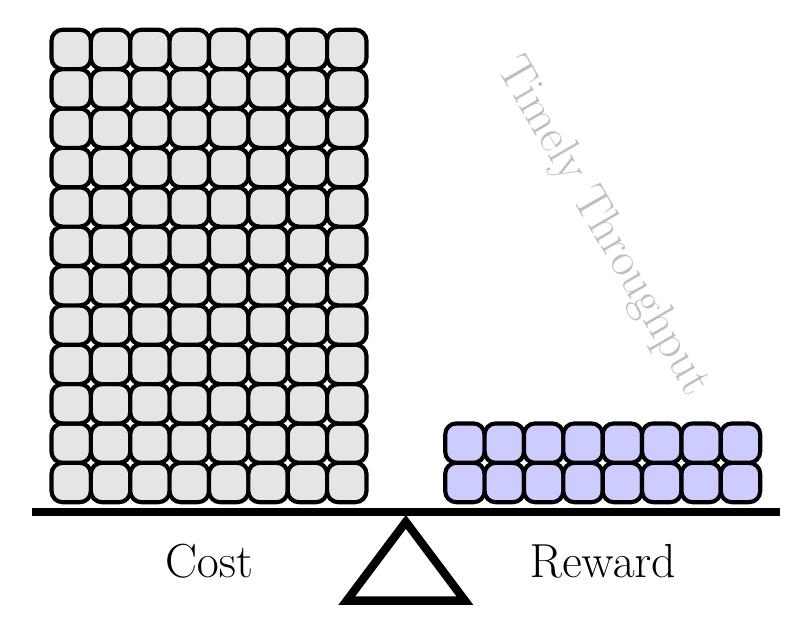
\begin{tikzpicture}
[draw=black, line width=1.5pt, >=stealth',
entry2/.style={rectangle, rounded corners, draw, fill=blue!20, inner sep=0pt, minimum size=5mm},
entry/.style={rectangle, rounded corners, draw, fill=gray!20, inner sep=0pt, minimum size=5mm}]

\node[entry] (m00) at (0,0) {};
\node[entry] (m01) at (0,0.5) {};
\node[entry] (m02) at (0,1) {};
\node[entry] (m03) at (0,1.5) {};
\node[entry] (m04) at (0,2) {};
\node[entry] (m05) at (0,2.5) {};
\node[entry] (m06) at (0,3) {};
\node[entry] (m07) at (0,3.5) {};
\node[entry] (m08) at (0,4) {};
\node[entry] (m09) at (0,4.5) {};
\node[entry] (m010) at (0,5) {};
\node[entry] (m011) at (0,5.5) {};

\node[entry] (m10) at (0.5,0) {};
\node[entry] (m11) at (0.5,0.5) {};
\node[entry] (m12) at (0.5,1) {};
\node[entry] (m13) at (0.5,1.5) {};
\node[entry] (m14) at (0.5,2) {};
\node[entry] (m15) at (0.5,2.5) {};
\node[entry] (m16) at (0.5,3) {};
\node[entry] (m17) at (0.5,3.5) {};
\node[entry] (m18) at (0.5,4) {};
\node[entry] (m19) at (0.5,4.5) {};
\node[entry] (m110) at (0.5,5) {};
\node[entry] (m111) at (0.5,5.5) {};

\node[entry] (m20) at (1,0) {};
\node[entry] (m21) at (1,0.5) {};
\node[entry] (m22) at (1,1) {};
\node[entry] (m23) at (1,1.5) {};
\node[entry] (m24) at (1,2) {};
\node[entry] (m25) at (1,2.5) {};
\node[entry] (m26) at (1,3) {};
\node[entry] (m27) at (1,3.5) {};
\node[entry] (m28) at (1,4) {};
\node[entry] (m29) at (1,4.5) {};
\node[entry] (m210) at (1,5) {};
\node[entry] (m211) at (1,5.5) {};

\node[entry] (m30) at (1.5,0) {};
\node[entry] (m31) at (1.5,0.5) {};
\node[entry] (m32) at (1.5,1) {};
\node[entry] (m33) at (1.5,1.5) {};
\node[entry] (m34) at (1.5,2) {};
\node[entry] (m35) at (1.5,2.5) {};
\node[entry] (m36) at (1.5,3) {};
\node[entry] (m37) at (1.5,3.5) {};
\node[entry] (m38) at (1.5,4) {};
\node[entry] (m39) at (1.5,4.5) {};
\node[entry] (m310) at (1.5,5) {};
\node[entry] (m311) at (1.5,5.5) {};

\node[entry] (m40) at (2,0) {};
\node[entry] (m41) at (2,0.5) {};
\node[entry] (m42) at (2,1) {};
\node[entry] (m43) at (2,1.5) {};
\node[entry] (m44) at (2,2) {};
\node[entry] (m45) at (2,2.5) {};
\node[entry] (m46) at (2,3) {};
\node[entry] (m47) at (2,3.5) {};
\node[entry] (m48) at (2,4) {};
\node[entry] (m49) at (2,4.5) {};
\node[entry] (m410) at (2,5) {};
\node[entry] (m411) at (2,5.5) {};

\node[entry] (m50) at (2.5,0) {};
\node[entry] (m51) at (2.5,0.5) {};
\node[entry] (m52) at (2.5,1) {};
\node[entry] (m53) at (2.5,1.5) {};
\node[entry] (m54) at (2.5,2) {};
\node[entry] (m55) at (2.5,2.5) {};
\node[entry] (m56) at (2.5,3) {};
\node[entry] (m57) at (2.5,3.5) {};
\node[entry] (m58) at (2.5,4) {};
\node[entry] (m59) at (2.5,4.5) {};
\node[entry] (m510) at (2.5,5) {};
\node[entry] (m511) at (2.5,5.5) {};

\node[entry] (m60) at (3,0) {};
\node[entry] (m61) at (3,0.5) {};
\node[entry] (m62) at (3,1) {};
\node[entry] (m63) at (3,1.5) {};
\node[entry] (m64) at (3,2) {};
\node[entry] (m65) at (3,2.5) {};
\node[entry] (m66) at (3,3) {};
\node[entry] (m67) at (3,3.5) {};
\node[entry] (m68) at (3,4) {};
\node[entry] (m69) at (3,4.5) {};
\node[entry] (m610) at (3,5) {};
\node[entry] (m611) at (3,5.5) {};

\node[entry] (m70) at (3.5,0) {};
\node[entry] (m71) at (3.5,0.5) {};
\node[entry] (m72) at (3.5,1) {};
\node[entry] (m73) at (3.5,1.5) {};
\node[entry] (m74) at (3.5,2) {};
\node[entry] (m75) at (3.5,2.5) {};
\node[entry] (m76) at (3.5,3) {};
\node[entry] (m77) at (3.5,3.5) {};
\node[entry] (m78) at (3.5,4) {};
\node[entry] (m79) at (3.5,4.5) {};
\node[entry] (m710) at (3.5,5) {};
\node[entry] (m711) at (3.5,5.5) {};

\node[entry2] (r00) at (5,0) {};
\node[entry2] (r01) at (5,0.5) {};

\node[entry2] (r10) at (5.5,0) {};
\node[entry2] (r11) at (5.5,0.5) {};

\node[entry2] (r20) at (6,0) {};
\node[entry2] (r21) at (6,0.5) {};

\node[entry2] (r30) at (6.5,0) {};
\node[entry2] (r31) at (6.5,0.5) {};

\node[entry2] (r40) at (7,0) {};
\node[entry2] (r41) at (7,0.5) {};

\node[entry2] (r50) at (7.5,0) {};
\node[entry2] (r51) at (7.5,0.5) {};

\node[entry2] (r60) at (8,0) {};
\node[entry2] (r61) at (8,0.5) {};

\node[entry2] (r70) at (8.5,0) {};
\node[entry2] (r71) at (8.5,0.5) {};

\draw[line width=3pt] (-0.5,-0.375) -- (9,-0.375);
\draw[line width=3pt] (3.5,-1.5) -- (4.25,-0.5) -- (5,-1.5) -- (3.5,-1.5) -- (4.25,-0.5);

\node (reward) at (1.75,-1) {\LARGE Cost};
\node (cost) at (6.75,-1) {\LARGE Reward};
\node[rotate=-60] (info) at (6.75,3.25) {\LARGE \textcolor{lightgray}{Timely Throughput}};
\end{tikzpicture}
}
  \end{center}
\end{columns}
\end{frame}


\begin{frame}{Uncoordinated Massive Multiple Access}
\begin{center}
  \scalebox{0.7}{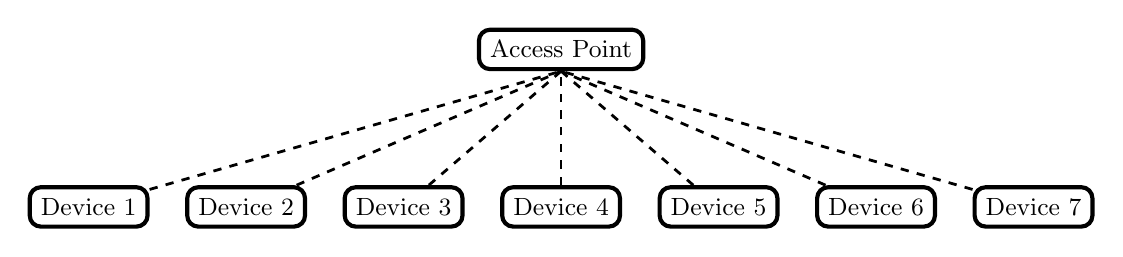
\begin{tikzpicture}
  [
  font=\small, line width=1pt, draw=black, >=stealth',
  bitnode/.style={rectangle, rounded corners, inner sep=4pt, minimum size=5mm, draw=black,line width=1.5pt},
  checknode/.style={rectangle, rounded corners, inner sep=4pt, minimum size=5mm, draw=black,line width=1.5pt},
  ]

  \node[bitnode] (b1) at (0,4) {Access Point};

  \foreach \x in {1,2,3,4,5,6,7} {
    \node[checknode] (c1\x) at (-8+2*\x,2) {Device~\x}
      edge[dashed] (b1.south);
  }

\end{tikzpicture}

}
\end{center}
\vfill
\begin{columns}
\column{.45\textwidth}
  \begin{center}
  \scalebox{0.45}{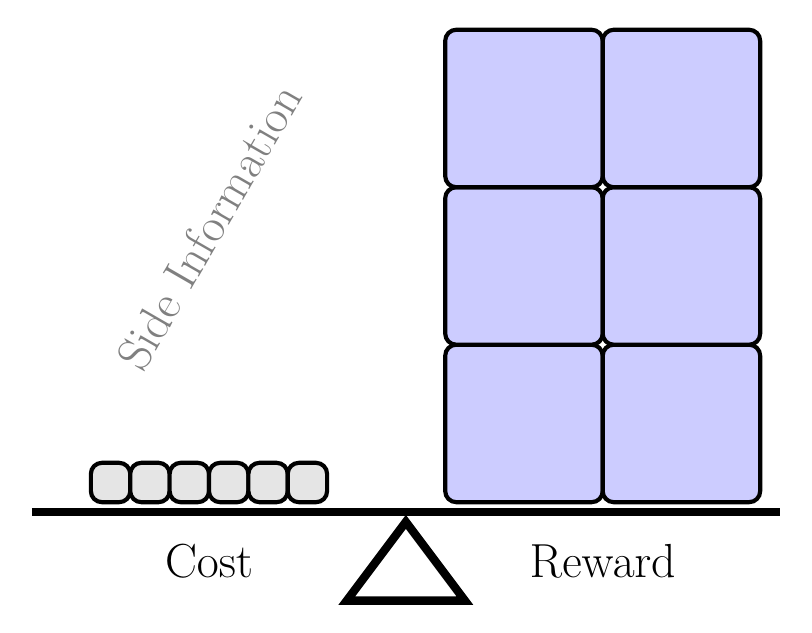
\begin{tikzpicture}
[draw=black, line width=1.5pt, >=stealth',
entry2/.style={rectangle, rounded corners, draw, fill=blue!20, inner sep=0pt, minimum size=20mm},
entry/.style={rectangle, rounded corners, draw, fill=gray!20, inner sep=0pt, minimum size=5mm}]

\node[entry] (r10) at (0.5,0) {};
\node[entry] (r20) at (1,0) {};
\node[entry] (r30) at (1.5,0) {};
\node[entry] (r40) at (2,0) {};
\node[entry] (r50) at (2.5,0) {};
\node[entry] (r60) at (3,0) {};

\node[entry2] (m00) at (5.75,0.75) {};
\node[entry2] (m01) at (5.75,2.75) {};
\node[entry2] (m02) at (5.75,4.75) {};
\node[entry2] (m00) at (7.75,0.75) {};
\node[entry2] (m11) at (7.75,2.75) {};
\node[entry2] (m12) at (7.75,4.75) {};

\draw[line width=3pt] (-0.5,-0.375) -- (9,-0.375);
\draw[line width=3pt] (3.5,-1.5) -- (4.25,-0.5) -- (5,-1.5) -- (3.5,-1.5) -- (4.25,-0.5);

\node (reward) at (1.75,-1) {\LARGE Cost};
\node (cost) at (6.75,-1) {\LARGE Reward};
\node[rotate=60] (info) at (1.75,3.25) {\LARGE \textcolor{gray}{Side Information}};
\end{tikzpicture}
}
  \end{center}
\column{.45\textwidth}
  \begin{center}
  \scalebox{0.45}{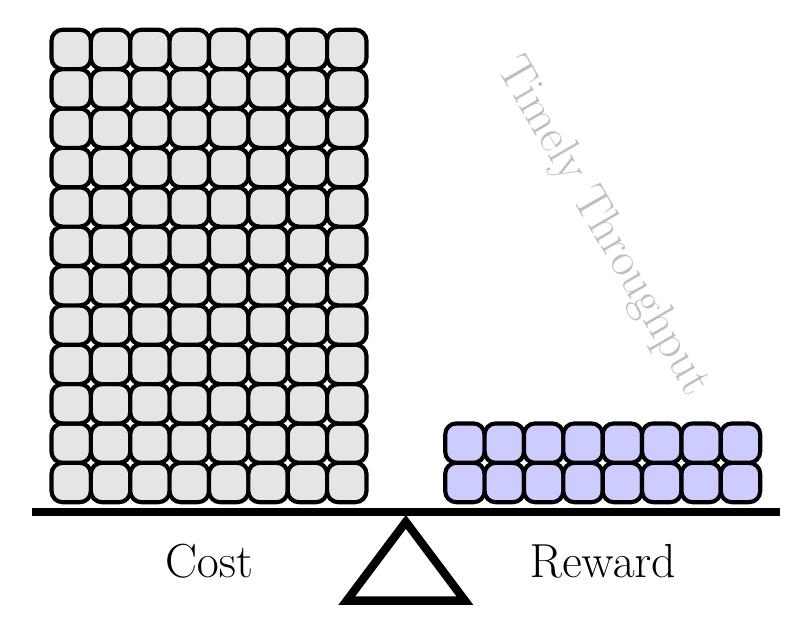
\begin{tikzpicture}
[draw=black, line width=1.5pt, >=stealth',
entry2/.style={rectangle, rounded corners, draw, fill=blue!20, inner sep=0pt, minimum size=5mm},
entry/.style={rectangle, rounded corners, draw, fill=gray!20, inner sep=0pt, minimum size=5mm}]

\node[entry] (m00) at (0,0) {};
\node[entry] (m01) at (0,0.5) {};
\node[entry] (m02) at (0,1) {};
\node[entry] (m03) at (0,1.5) {};
\node[entry] (m04) at (0,2) {};
\node[entry] (m05) at (0,2.5) {};
\node[entry] (m06) at (0,3) {};
\node[entry] (m07) at (0,3.5) {};
\node[entry] (m08) at (0,4) {};
\node[entry] (m09) at (0,4.5) {};
\node[entry] (m010) at (0,5) {};
\node[entry] (m011) at (0,5.5) {};

\node[entry] (m10) at (0.5,0) {};
\node[entry] (m11) at (0.5,0.5) {};
\node[entry] (m12) at (0.5,1) {};
\node[entry] (m13) at (0.5,1.5) {};
\node[entry] (m14) at (0.5,2) {};
\node[entry] (m15) at (0.5,2.5) {};
\node[entry] (m16) at (0.5,3) {};
\node[entry] (m17) at (0.5,3.5) {};
\node[entry] (m18) at (0.5,4) {};
\node[entry] (m19) at (0.5,4.5) {};
\node[entry] (m110) at (0.5,5) {};
\node[entry] (m111) at (0.5,5.5) {};

\node[entry] (m20) at (1,0) {};
\node[entry] (m21) at (1,0.5) {};
\node[entry] (m22) at (1,1) {};
\node[entry] (m23) at (1,1.5) {};
\node[entry] (m24) at (1,2) {};
\node[entry] (m25) at (1,2.5) {};
\node[entry] (m26) at (1,3) {};
\node[entry] (m27) at (1,3.5) {};
\node[entry] (m28) at (1,4) {};
\node[entry] (m29) at (1,4.5) {};
\node[entry] (m210) at (1,5) {};
\node[entry] (m211) at (1,5.5) {};

\node[entry] (m30) at (1.5,0) {};
\node[entry] (m31) at (1.5,0.5) {};
\node[entry] (m32) at (1.5,1) {};
\node[entry] (m33) at (1.5,1.5) {};
\node[entry] (m34) at (1.5,2) {};
\node[entry] (m35) at (1.5,2.5) {};
\node[entry] (m36) at (1.5,3) {};
\node[entry] (m37) at (1.5,3.5) {};
\node[entry] (m38) at (1.5,4) {};
\node[entry] (m39) at (1.5,4.5) {};
\node[entry] (m310) at (1.5,5) {};
\node[entry] (m311) at (1.5,5.5) {};

\node[entry] (m40) at (2,0) {};
\node[entry] (m41) at (2,0.5) {};
\node[entry] (m42) at (2,1) {};
\node[entry] (m43) at (2,1.5) {};
\node[entry] (m44) at (2,2) {};
\node[entry] (m45) at (2,2.5) {};
\node[entry] (m46) at (2,3) {};
\node[entry] (m47) at (2,3.5) {};
\node[entry] (m48) at (2,4) {};
\node[entry] (m49) at (2,4.5) {};
\node[entry] (m410) at (2,5) {};
\node[entry] (m411) at (2,5.5) {};

\node[entry] (m50) at (2.5,0) {};
\node[entry] (m51) at (2.5,0.5) {};
\node[entry] (m52) at (2.5,1) {};
\node[entry] (m53) at (2.5,1.5) {};
\node[entry] (m54) at (2.5,2) {};
\node[entry] (m55) at (2.5,2.5) {};
\node[entry] (m56) at (2.5,3) {};
\node[entry] (m57) at (2.5,3.5) {};
\node[entry] (m58) at (2.5,4) {};
\node[entry] (m59) at (2.5,4.5) {};
\node[entry] (m510) at (2.5,5) {};
\node[entry] (m511) at (2.5,5.5) {};

\node[entry] (m60) at (3,0) {};
\node[entry] (m61) at (3,0.5) {};
\node[entry] (m62) at (3,1) {};
\node[entry] (m63) at (3,1.5) {};
\node[entry] (m64) at (3,2) {};
\node[entry] (m65) at (3,2.5) {};
\node[entry] (m66) at (3,3) {};
\node[entry] (m67) at (3,3.5) {};
\node[entry] (m68) at (3,4) {};
\node[entry] (m69) at (3,4.5) {};
\node[entry] (m610) at (3,5) {};
\node[entry] (m611) at (3,5.5) {};

\node[entry] (m70) at (3.5,0) {};
\node[entry] (m71) at (3.5,0.5) {};
\node[entry] (m72) at (3.5,1) {};
\node[entry] (m73) at (3.5,1.5) {};
\node[entry] (m74) at (3.5,2) {};
\node[entry] (m75) at (3.5,2.5) {};
\node[entry] (m76) at (3.5,3) {};
\node[entry] (m77) at (3.5,3.5) {};
\node[entry] (m78) at (3.5,4) {};
\node[entry] (m79) at (3.5,4.5) {};
\node[entry] (m710) at (3.5,5) {};
\node[entry] (m711) at (3.5,5.5) {};

\node[entry2] (r00) at (5,0) {};
\node[entry2] (r01) at (5,0.5) {};

\node[entry2] (r10) at (5.5,0) {};
\node[entry2] (r11) at (5.5,0.5) {};

\node[entry2] (r20) at (6,0) {};
\node[entry2] (r21) at (6,0.5) {};

\node[entry2] (r30) at (6.5,0) {};
\node[entry2] (r31) at (6.5,0.5) {};

\node[entry2] (r40) at (7,0) {};
\node[entry2] (r41) at (7,0.5) {};

\node[entry2] (r50) at (7.5,0) {};
\node[entry2] (r51) at (7.5,0.5) {};

\node[entry2] (r60) at (8,0) {};
\node[entry2] (r61) at (8,0.5) {};

\node[entry2] (r70) at (8.5,0) {};
\node[entry2] (r71) at (8.5,0.5) {};

\draw[line width=3pt] (-0.5,-0.375) -- (9,-0.375);
\draw[line width=3pt] (3.5,-1.5) -- (4.25,-0.5) -- (5,-1.5) -- (3.5,-1.5) -- (4.25,-0.5);

\node (reward) at (1.75,-1) {\LARGE Cost};
\node (cost) at (6.75,-1) {\LARGE Reward};
\node[rotate=-60] (info) at (6.75,3.25) {\LARGE \textcolor{lightgray}{Timely Throughput}};
\end{tikzpicture}
}
  \end{center}
\end{columns}
\end{frame}


\begin{frame}{Possible MAC Frame Structure}
\begin{itemize}
\item $K$ active devices out of $Q$ devices
\item $Q$ is very large, and $K$ is much less than $Q$
\end{itemize}
\begin{center}
  \scalebox{0.8}{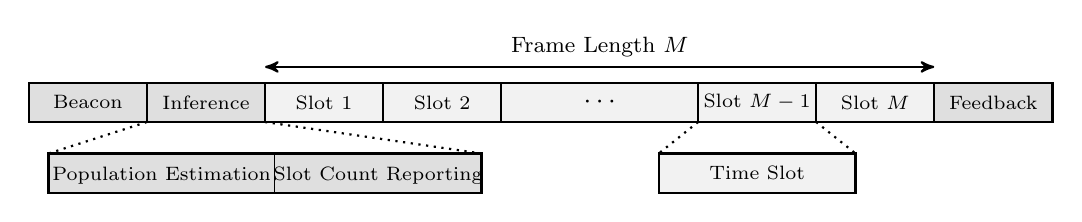
\begin{tikzpicture}[>=stealth', thick]

% --------
\draw [fill=gray!10] (0,0) rectangle (13,0.5);
\draw [<->] (3,0.7) -- node[above]{\footnotesize Frame Length $M$} (11.5,0.7);

\draw [fill=gray!25] (0,0) rectangle (1.5,0.5);
\node at (0.75,0.25) {\scriptsize Beacon};

\draw [fill=gray!25] (1.5,0) rectangle (3,0.5);
\node at (2.25,0.25) {\scriptsize Inference};

\draw (3,0) -- (3,0.5);
\draw (4.5,0) -- (4.5,0.5);
\draw (6,0) -- (6,0.5);
\draw (8.5,0) -- (8.5,0.5);
\draw (10,0) -- (10,0.5);
\draw (11.5,0) -- (11.5,0.5);

\node at (3.75,0.25) {\scriptsize Slot~$1$};
\node at (5.25,0.25) {\scriptsize Slot~$2$};
\node at (7.25,0.25) {$\cdots$};
\node at (9.25,0.25) {\scriptsize Slot~$M - 1$};
\node at (10.75,0.25) {\scriptsize Slot~$M$};

\draw [fill=gray!25] (11.5,0) rectangle (13,0.5);
\node at (12.25,0.25) {\scriptsize Feedback};

% --------
\draw [fill=gray!10] (8,-0.9) rectangle (10.5,-0.4);
\draw [dotted] (8.5,0)--(8,-0.4);
\draw [dotted] (10,0)--(10.5,-0.4);
\node at (9.25,-0.65) {\scriptsize Time Slot};

% --------
\draw [fill=gray!25] (0.25,-0.9) rectangle (5.75,-0.4);
\node at (1.6875,-0.675) {\scriptsize Population Estimation};
\node at (4.4375,-0.675) {\scriptsize Slot Count Reporting};
\draw [dotted] (1.5,0)--(0.25,-0.4);
\draw [dotted] (3,0)--(5.75,-0.4);
\draw[thin] (3.125,-0.4) -- (3.125,-0.9);

\end{tikzpicture} 

}
\end{center}
\begin{itemize}
\item Beacon is used to obtain coarse synchronization
\item Each device transmits a signature sequence
\item Access point estimates \# of devices $K$
\item Picks frame length $M$ and inform devices
\end{itemize}
\footnotetext[1]{X. Chen and D. Guo. ``Many-access channels: The Gaussian case with random user activities.'' ISIT, 2014.}
\end{frame}


\begin{frame}
\frametitle{Random Access -- Revisiting the Tradition}
\begin{center}
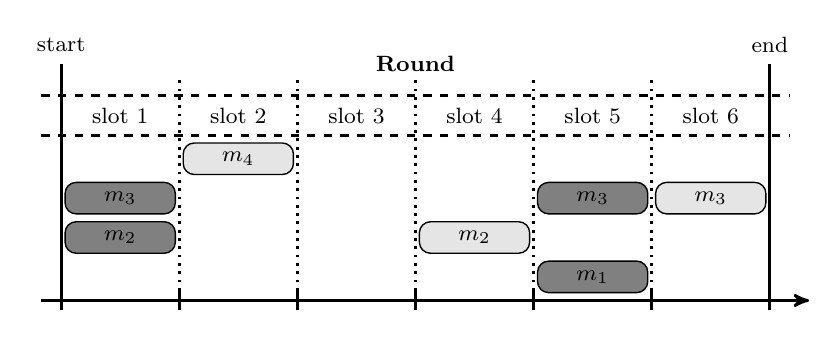
\begin{tikzpicture}[
  font=\footnotesize,
  >=stealth',
  line width=1pt,
  packet/.style={rectangle, minimum height=4mm, minimum width=14mm, draw=black, fill=gray!20, rounded corners, line width=0.5pt}
]

\draw [->] (0,-0.05) -- (9.75,-0.05);
\draw (0.25,-0.175) -- (0.25,2.95);
\foreach \x in {1,...,5} {
  \draw (1.5*\x+0.25,-0.175) -- (1.5*\x+0.25,0.075);
  \draw[dotted] (1.5*\x+0.25,0.075) -- (1.5*\x+0.25,2.75);
}
\draw (9.25,-0.175) -- (9.25,2.95);
\draw[dashed] (0,2.05) -- (9.5,2.05);
\draw[dashed] (0,2.55) -- (9.5,2.55);

\foreach \x in {1,...,6} {
  \node (t\x) at (1.5*\x-0.5,2.3) {slot~\x};
}
\node (round) at (4.75,2.95) {\textbf{Round}};
\node (start) at (0.25,3.2) {start};
\node (end) at (9.25,3.2) {end};

%\node[packet] (p12) at (2.5,0.25) {$m_1$};
\node[packet,fill=gray] (p15) at (7.0,0.25) {$m_1$};
\node[packet,fill=gray] (p21) at (1.0,0.75) {$m_2$};
%\node[packet] (p23) at (4.0,0.75) {$m_2$};
\node[packet] (p24) at (5.5,0.75) {$m_2$};
\node[packet,fill=gray] (p31) at (1.0,1.25) {$m_3$};
\node[packet,fill=gray] (p35) at (7.0,1.25) {$m_3$};
\node[packet] (p36) at (8.5,1.25) {$m_3$};
\node[packet] (p42) at (2.5,1.75) {$m_4$};
%\node[packet] (p43) at (4.0,1.75) {$m_4$};
%\node[packet] (p45) at (7.0,1.75) {$m_4$};

\end{tikzpicture}


\end{center}
\begin{block}{Slotted ALOHA}
  \begin{itemize}
  \item $K$ \textbf{uncoordinated} devices
  \item Time is \textbf{slotted}; transmissions occur within slots
  \item Collided packets are discarded
  \item Receiver provides \textbf{feedback} about collision events
  \item Back-off strategy determines performance, bounded by $1/e \approx 0.37$
  \end{itemize}
\end{block}
\footnotetext[1]{\scriptsize{N. Abramson, ``The ALOHA system: Another alternative for computer communications,'' in Proc.\ Computer Conference (1970).}}
\end{frame}


\begin{frame}
\frametitle{Random Access with Twist}
\begin{center}
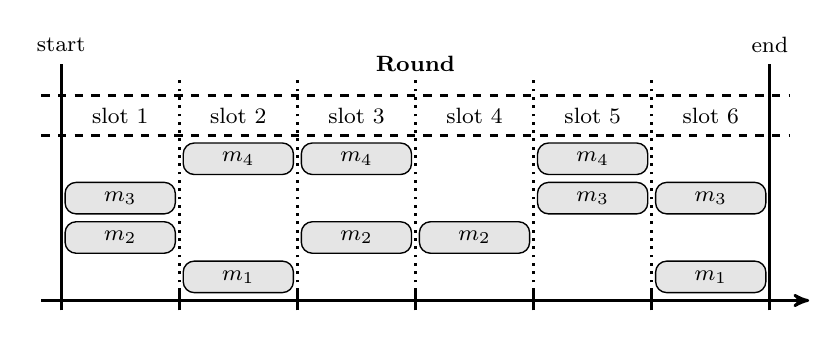
\begin{tikzpicture}[
  font=\footnotesize,
  >=stealth',
  line width=1pt,
  packet/.style={rectangle, minimum height=4mm, minimum width=14mm, draw=black, fill=gray!20, rounded corners, line width=0.5pt}
]

\draw [->] (0,-0.05) -- (9.75,-0.05);
\draw (0.25,-0.175) -- (0.25,2.95);
\foreach \x in {1,...,5} {
  \draw (1.5*\x+0.25,-0.175) -- (1.5*\x+0.25,0.075);
  \draw[dotted] (1.5*\x+0.25,0.075) -- (1.5*\x+0.25,2.75);
}
\draw (9.25,-0.175) -- (9.25,2.95);
\draw[dashed] (0,2.05) -- (9.5,2.05);
\draw[dashed] (0,2.55) -- (9.5,2.55);

\foreach \x in {1,...,6} {
  \node (t\x) at (1.5*\x-0.5,2.3) {slot~\x};
}
\node (round) at (4.75,2.95) {\textbf{Round}};
\node (start) at (0.25,3.2) {start};
\node (end) at (9.25,3.2) {end};

\node[packet] (p12) at (2.5,0.25) {$m_1$};
\node[packet] (p16) at (8.5,0.25) {$m_1$};
\node[packet] (p21) at (1.0,0.75) {$m_2$};
\node[packet] (p23) at (4.0,0.75) {$m_2$};
\node[packet] (p24) at (5.5,0.75) {$m_2$};
\node[packet] (p31) at (1.0,1.25) {$m_3$};
\node[packet] (p35) at (7.0,1.25) {$m_3$};
\node[packet] (p36) at (8.5,1.25) {$m_3$};
\node[packet] (p42) at (2.5,1.75) {$m_4$};
\node[packet] (p43) at (4.0,1.75) {$m_4$};
\node[packet] (p45) at (7.0,1.75) {$m_4$};

\end{tikzpicture}


\end{center}
\begin{block}{System Model}
  \begin{itemize}
  \item $K$ \textbf{uncoordinated} devices, each with 1 packet to send
  \item Time is \textbf{slotted}; transmissions occur within slots
  \item Receiver knows full schedule, collection of packets in every slot
  \item Successive interference cancellation
  \end{itemize}
\end{block}
\footnotetext[1]{\scriptsize  E. Casini, R. De Gaudenzi, and O. Del Rio Herrero. ``Contention resolution diversity slotted ALOHA (CRDSA): An enhanced random access scheme for satellite access packet networks.'' IEEE Trans.\ on Wireless Communications (2007).}
\end{frame}


\begin{frame}
\frametitle{Graphical Representation}
\begin{itemize}
\item Tanner graph representation for transmission scheme
\item Variable nodes $\leftrightarrow$ packets;
Check nodes $\leftrightarrow$ received signals
\item Message-passing decoder (SIC) -- \textbf{peeling decoder} for erasure channel
\end{itemize}
\begin{columns}
\column{.48\textwidth}
  \begin{center}
  \scalebox{0.8}{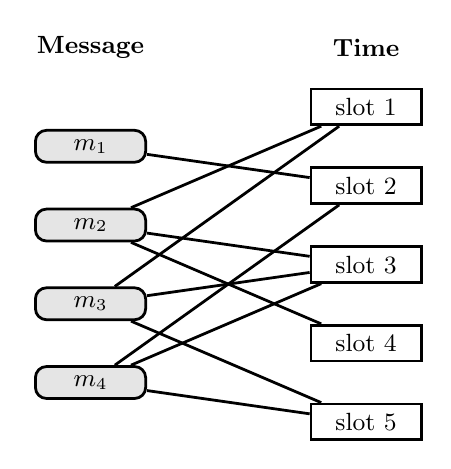
\begin{tikzpicture}
  [
  font=\small, line width=1pt, draw=black,
  checknode/.style={rectangle, minimum height=4mm, minimum width=14mm, draw=black},
  packet/.style={rectangle, minimum height=4mm, minimum width=14mm, draw=black, fill=gray!20, rounded corners}
  ]

\foreach \m in {1,2,3,4} {
  \node[packet] (v\m) at (0,0.5-\m) {$m_{\m}$};
}
  
\foreach \s in {1,2,3,4,5} {
  \node[checknode] (c\s) at (3.5,1-\s) {slot~\s};
}

\node (message) at (0,0.75) {\textbf{Message}};
\node (time) at (3.5,0.75) {\textbf{Time}};

\draw (v1) -- (c2);
\draw (v2) -- (c1);
\draw (v2) -- (c3);
\draw (v2) -- (c4);
\draw (v3) -- (c1);
\draw (v3) -- (c3);
\draw (v3) -- (c5);
\draw (v4) -- (c2);
\draw (v4) -- (c3);
\draw (v4) -- (c5);
\end{tikzpicture}
}
  \end{center}
\column{.48\textwidth}
  \begin{center}
  \scalebox{0.8}{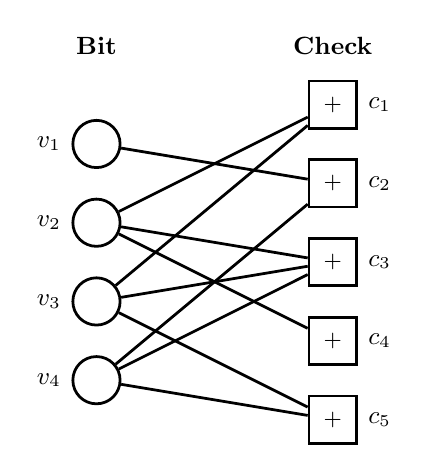
\begin{tikzpicture}
  [
  font=\small, line width=1pt, draw=black,
  bitnode/.style={circle, inner sep = 0pt, minimum size = 6mm, draw=black},
  checknode/.style={rectangle, inner sep = 0pt, minimum size = 6mm, draw=black},
  ]

\foreach \v in {1,2,3,4} {
  \node[bitnode] (v\v) at (0,0.5-\v) [label=left:$v_\v$]{};
}
  
\foreach \c in {1,2,3,4,5} {
  \node[checknode] (c\c) at (3,1-\c) [label=right:$c_\c$]{\footnotesize{$+$}};
}

\node (bit) at (0,0.75) {\textbf{Bit}};
\node (check) at (3,0.75) {\textbf{Check}};

\draw (v1) -- (c2);
\draw (v2) -- (c1);
\draw (v2) -- (c3);
\draw (v2) -- (c4);
\draw (v3) -- (c1);
\draw (v3) -- (c3);
\draw (v3) -- (c5);
\draw (v4) -- (c2);
\draw (v4) -- (c3);
\draw (v4) -- (c5);
\end{tikzpicture}

}
  \end{center}
\end{columns}
\footnotetext[1]{\scriptsize G. Liva. ``Graph-based analysis and optimization of contention resolution diversity slotted ALOHA.'' IEEE Trans.\ on Communications (2011).}
\footnotetext[2]{\scriptsize  E. Paolini, G. Liva, and M. Chiani. ``Coded slotted ALOHA: A graph-based method for uncoordinated multiple access.'' IEEE Trans.\ on Information Theory (2015).}
\end{frame}


\begin{frame}
\frametitle{Decoder -- Peeling Algorithm}
Joint decoding via successive interference cancellation
  \begin{center}
  \scalebox{1}{\pgfdeclarelayer{background}
\pgfdeclarelayer{foreground}

\pgfsetlayers{background,foreground}

\begin{tikzpicture}[
  line width=1pt, font=\footnotesize, >=stealth', draw=black,
  device/.style={circle, inner sep = 0pt, minimum height = 5mm, minimum width=5mm, draw=black, fill=gray!40, line width=0.5pt},
    decodeddevice/.style={circle, inner sep = 0pt, minimum height = 5mm, minimum width=5mm, draw=black, fill=blue, line width=0.5pt},
  slot/.style={rectangle, inner sep=0pt, minimum size=1.5mm, fill=black},
  packet/.style={rectangle, minimum height=4mm, minimum width=14mm, draw=black, fill=gray!20, rounded corners, line width=0.5pt},
    decodedpacket/.style={rectangle, minimum height=4mm, minimum width=14mm, draw=black, pattern=north east lines, rounded corners, line width=0.5pt}
]
\def\lw{1pt}

\begin{pgfonlayer}{background}
\draw [->,line width=1.25pt] (0,-0.05) -- (8.25,-0.05);
\draw[line width=1.25pt] (0.25,-0.175) -- (0.25,2.45);
\foreach \x in {1,...,4} {
  \draw (1.5*\x+0.25,-0.175) -- (1.5*\x+0.25,0.075);
  \draw[dotted,line width=1.25pt] (1.5*\x+0.25,0.075) -- (1.5*\x+0.25,2.25);
}
\draw[line width=1.25pt] (7.75,-0.175) -- (7.75,2.45);
\draw[dashed,line width=1.25pt] (0,2.05) -- (8,2.05);

\foreach \x in {1,...,5} {
  \node[slot] (s\x) at (1.5*\x-0.5,-0.3) {};
  \node (t\x) at (1.5*\x-0.5,2.3) {slot~\x};
}
\end{pgfonlayer}


\begin{pgfonlayer}{foreground}

\only<1>{\node (text) at (4,-3.5) {\large{Instance of Random Access}};}
\only<1>{
\node[device] (d2) at (3,-2) [label=below:device~2]{};
\node[packet] (p24) at (5.5,0.75) {$m_2$};
\draw[draw=gray, line width=\lw] (d2) -- (s4);
}

\only<2-3>{\node at (text) {\large{Step 1}};}
\only<2->{
\node[device, fill=red!30!blue!60] (d2) at (3,-2) [label=below:device~2]{};
\node[packet, fill=red!30!blue!60] (p24) at (5.5,0.75) {$m_2$};
\draw[draw=black, line width=\lw] (d2) -- (s4);
}

\only<1-3>{
\node[device] (d3) at (4.75,-2) [label=below:device~3]{};
\node[packet] (p31) at (1.0,1.25) {$m_3$};
\draw[draw=gray, line width=\lw] (d3) -- (s1);
}

\only<4-5>{\node at (text) {\large{Step 2}};}
\only<4->{
\node[device, fill=red!60!blue!30] (d3) at (4.75,-2) [label=below:device~3]{};
\node[packet, fill=red!60!blue!30] (p31) at (1.0,1.25) {$m_3$};
\draw[draw=black, line width=\lw] (d3) -- (s1);
}

\only<1-5>{
\node[device] (d4) at (6.5,-2) [label=below:device~4]{};
\node[packet] (p43) at (4.0,1.75) {$m_4$};
\node[packet] (p45) at (7.0,1.75) {$m_4$};
\draw[draw=gray, line width=\lw] (d4) -- (s3);
\draw[draw=gray, line width=\lw] (d4) -- (s5);
}

\only<6-7>{\node at (text) {\large{Step 3}};}
\only<6->{
\node[device, fill=red!50] (d4) at (6.5,-2) [label=below:device~4]{};
\node[packet, fill=red!50] (p43) at (4.0,1.75) {$m_4$};
\node[packet, fill=red!50] (p45) at (7.0,1.75) {$m_4$};
\draw[draw=black, line width=\lw] (d4) -- (s3);
\draw[draw=black, line width=\lw] (d4) -- (s5);
}

\only<1-7>{
\node[device] (d1) at (1.25,-2) [label=below:device~1]{};
\node[packet] (p12) at (2.5,0.25) {$m_1$};
\draw[draw=gray, line width=\lw] (d1) -- (s2);
}

\only<8>{\node at (text) {\large{Step 4}};}
\only<8->{
\node[device, fill=blue!50] (d1) at (1.25,-2) [label=below:device~1]{};
\node[packet, fill=blue!50] (p12) at (2.5,0.25) {$m_1$};
\draw[draw=black, line width=\lw] (d1) -- (s2);
}

\only<1-2>{
\node[packet] (p21) at (1.0,0.75) {$m_2$};
\node[packet] (p23) at (4.0,0.75) {$m_2$};
\draw[draw=gray, line width=\lw] (d2) -- (s1);
\draw[draw=gray, line width=\lw] (d2) -- (s3);
}

\only<3>{
\node[packet, fill=white, dashed] (p21) at (1.0,0.75) {};
\node[packet, fill=white, dashed] (p23) at (4.0,0.75) {};
\draw[draw=gray, line width=\lw, dashed] (d2) -- (s1);
\draw[draw=gray, line width=\lw, dashed] (d2) -- (s3);
}

\only<1-4>{
\node[packet] (p33) at (4.0,1.25) {$m_3$};
\node[packet] (p35) at (7.0,1.25) {$m_3$};
\draw[draw=gray, line width=\lw] (d3) -- (s3);
\draw[draw=gray, line width=\lw] (d3) -- (s5);
}

\only<5>{
\node[packet, fill=white, dashed] (p33) at (4.0,1.25) {};
\node[packet, fill=white, dashed] (p35) at (7.0,1.25) {};
\draw[draw=gray, line width=\lw, dashed] (d3) -- (s3);
\draw[draw=gray, line width=\lw, dashed] (d3) -- (s5);
}

\only<1-6>{
\node[packet] (p42) at (2.5,1.75) {$m_4$};
\draw[draw=gray, line width=\lw] (d4) -- (s2);
}

\only<7>{
\node[packet, fill=white, dashed] (p42) at (2.5,1.75) {};
\draw[draw=gray, line width=\lw, dashed] (d4) -- (s2);
}

\end{pgfonlayer}
\end{tikzpicture}

}
  \end{center}
\end{frame}


\begin{frame}
\frametitle{Representations: Schedule, Tanner Graph, Compressed}
\begin{center}
  \scalebox{1}{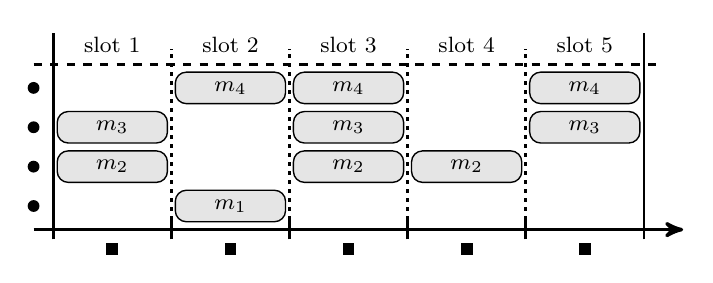
\begin{tikzpicture}[
  line width=1pt, font=\footnotesize, >=stealth', draw=black,
  packet/.style={rectangle, minimum height=4mm, minimum width=14mm, draw=black, fill=gray!20, rounded corners, line width=0.5pt},
  check/.style={rectangle, inner sep=0pt, minimum size=1.5mm, fill=black},
  varnode/.style={circle, inner sep=0pt, minimum size=1.5mm, fill=black}
]

\draw [->,line width=1.25pt] (0,-0.05) -- (8.25,-0.05);
\draw[line width=1.25pt] (0.25,-0.175) -- (0.25,2.45);
\foreach \x in {1,...,4} {
  \draw (1.5*\x+0.25,-0.175) -- (1.5*\x+0.25,0.075);
  \draw[dotted,line width=1.25pt] (1.5*\x+0.25,0.075) -- (1.5*\x+0.25,2.25);
}

\foreach \v in {1,...,4} {
  \node[varnode] (v\v) at (0,0.5*\v-0.25) {};
}

\foreach \x in {1,...,5} {
  \node[check] (c\x) at (1.5*\x-0.5,-0.3) {};
  \node (t\x) at (1.5*\x-0.5,2.3) {slot~\x};
}

\draw[thick] (7.75,-0.175) -- (7.75,2.45);
\draw[dashed,line width=1.25pt] (0,2.05) -- (8,2.05);

\node[packet] (p12) at (2.5,0.25) {$m_1$};
\node[packet] (p21) at (1.0,0.75) {$m_2$};
\node[packet] (p23) at (4.0,0.75) {$m_2$};
\node[packet] (p24) at (5.5,0.75) {$m_2$};
\node[packet] (p31) at (1.0,1.25) {$m_3$};
\node[packet] (p33) at (4.0,1.25) {$m_3$};
\node[packet] (p35) at (7.0,1.25) {$m_3$};
\node[packet] (p42) at (2.5,1.75) {$m_4$};
\node[packet] (p43) at (4.0,1.75) {$m_4$};
\node[packet] (p45) at (7.0,1.75) {$m_4$};

\end{tikzpicture}

}
\end{center}
\begin{columns}
\column{.45\textwidth}
  \begin{center}
  \scalebox{0.8}{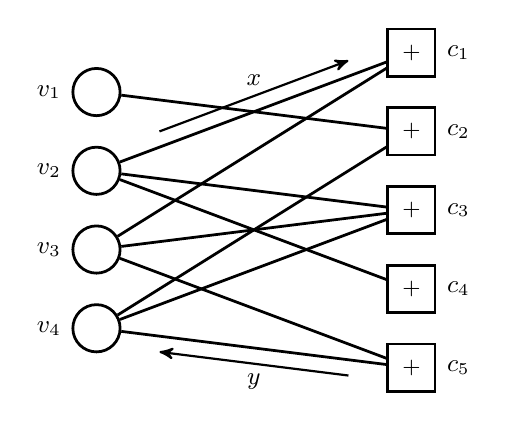
\begin{tikzpicture}
  [
  font=\small,
  line width=1pt,
  node distance = 3mm, draw=black, >=stealth',
  bitnode/.style={circle, inner sep = 0pt, minimum size = 6mm, draw=black},
  checknode/.style={rectangle, inner sep = 0pt, minimum size = 6mm, draw=black},
  ]

  \foreach \y in {1,2,3,4} {
    \node[bitnode] (b\y) at (0,0.5-\y) [label=left:$v_\y$]{};
  }
  
  \foreach \y in {1,2,3,4,5} {
    \node[checknode] (c\y) at (4,1-\y) [label=right:$c_\y$]{\footnotesize{$+$}};
  }

  \draw (b1) -- (c2);
  \draw (b2) -- (c1);
  \draw (b2) -- (c3);
  \draw (b2) -- (c4);
  \draw (b3) -- (c1);
  \draw (b3) -- (c3);
  \draw (b3) -- (c5);
  \draw (b4) -- (c2);
  \draw (b4) -- (c3);
  \draw (b4) -- (c5);

%  \draw[thick] (0,-1.5) -- (4,0);
%  \draw[thick] (0.8,-1.2) -- (3.2,-0.3);
  \draw[->,thick] (0.8,-1) -- node[above] {$x$} (3.2,-0.1);

%  \draw[thick] (0,-3.5) -- (4,-4);
%  \draw[thick] (0.8,-3.6) -- (3.2,-3.9);
  \draw[<-,thick] (0.8,-3.8) -- node[below] {$y$} (3.2,-4.1);

\end{tikzpicture}
}
  \end{center}
\column{.45\textwidth}
  \begin{center}
  \scalebox{0.8}{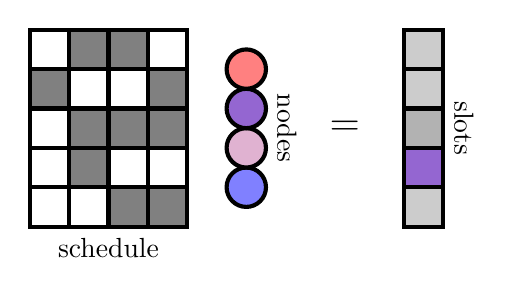
\begin{tikzpicture}
[draw=black, line width=1.5pt, >=stealth',
entry1/.style={rectangle, draw, fill=gray, inner sep=0pt, minimum size=5mm},
entry0/.style={rectangle, draw, inner sep=0pt, minimum size=5mm},
symbol/.style={circle, draw, inner sep=0pt, minimum size=5mm}]

\node[anchor=north] (schedule) at (0.75,-0.25) {schedule};
\node[entry0] (m00) at (0,0) {};
\node[entry0] (m01) at (0.5,0) {};
\node[entry1] (m02) at (1,0) {};
\node[entry1] (m03) at (1.5,0) {};

\node[entry0] (m00) at (0,0.5) {};
\node[entry1] (m11) at (0.5,0.5) {};
\node[entry0] (m12) at (1,0.5) {};
\node[entry0] (m13) at (1.5,0.5) {};

\node[entry0] (m20) at (0,1) {};
\node[entry1] (m21) at (0.5,1) {};
\node[entry1] (m22) at (1,1) {};
\node[entry1] (m23) at (1.5,1) {};

\node[entry1] (m30) at (0,1.5) {};
\node[entry0] (m31) at (0.5,1.5) {};
\node[entry0] (m32) at (1,1.5) {};
\node[entry1] (m33) at (1.5,1.5) {};

\node[entry0] (m40) at (0,2) {};
\node[entry1] (m41) at (0.5,2) {};
\node[entry1] (m42) at (1,2) {};
\node[entry0] (m43) at (1.5,2) {};

\node[symbol,fill=blue!50] (s1) at (2.5,0.25) {};
\node[symbol,fill=red!60!blue!30] (s2) at (2.5,0.75) {};
\node[symbol,fill=red!30!blue!60] (s3) at (2.5,1.25) {};
\node[symbol,fill=red!50] (s4) at (2.5,1.75) {};
\node[anchor=south,rotate=-90] (variables) at (2.75,1) {nodes};


\node (equal) at (3.75,1) {\Large =};

\node[entry0,fill=black!20] (y0) at (4.75,0) {};
\node[entry0,fill=red!30!blue!60] (y1) at (4.75,0.5) {};
\node[entry0,fill=black!30] (y2) at (4.75,1) {};
\node[entry0,fill=black!20] (y3) at (4.75,1.5) {};
\node[entry0,fill=black!20] (y4) at (4.75,2) {};
\node[anchor=south,rotate=-90] (slots) at (5,1) {slots};

\end{tikzpicture}

}
  \end{center}
\end{columns}
\end{frame}


\begin{frame}
\frametitle{Graphical Methods: Tools from Iterative Decoding}
\begin{itemize}
\item $L(z) = \sum_i L_i z^i$ variable dist.\ from node
\item $\lambda(z) = \sum_i \lambda_i x^{i-1} = {L'(z)}/{L'(1)}$ variable dist.\ from edge
\item $R(z) = \sum_j R_j z^i$ check dist.\ from node
\item $\rho(z) = \sum_j \rho_j x^{j-1} = {R'(z)}/{R'(1)}$ check dist.\ from edge
\end{itemize}
\begin{columns}
\column{.45\textwidth}
  \begin{center}
  \scalebox{0.8}{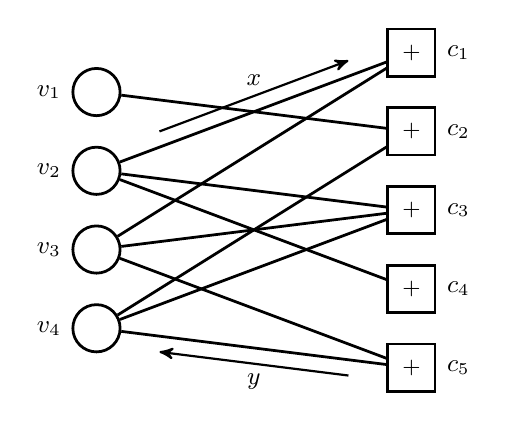
\begin{tikzpicture}
  [
  font=\small,
  line width=1pt,
  node distance = 3mm, draw=black, >=stealth',
  bitnode/.style={circle, inner sep = 0pt, minimum size = 6mm, draw=black},
  checknode/.style={rectangle, inner sep = 0pt, minimum size = 6mm, draw=black},
  ]

  \foreach \y in {1,2,3,4} {
    \node[bitnode] (b\y) at (0,0.5-\y) [label=left:$v_\y$]{};
  }
  
  \foreach \y in {1,2,3,4,5} {
    \node[checknode] (c\y) at (4,1-\y) [label=right:$c_\y$]{\footnotesize{$+$}};
  }

  \draw (b1) -- (c2);
  \draw (b2) -- (c1);
  \draw (b2) -- (c3);
  \draw (b2) -- (c4);
  \draw (b3) -- (c1);
  \draw (b3) -- (c3);
  \draw (b3) -- (c5);
  \draw (b4) -- (c2);
  \draw (b4) -- (c3);
  \draw (b4) -- (c5);

%  \draw[thick] (0,-1.5) -- (4,0);
%  \draw[thick] (0.8,-1.2) -- (3.2,-0.3);
  \draw[->,thick] (0.8,-1) -- node[above] {$x$} (3.2,-0.1);

%  \draw[thick] (0,-3.5) -- (4,-4);
%  \draw[thick] (0.8,-3.6) -- (3.2,-3.9);
  \draw[<-,thick] (0.8,-3.8) -- node[below] {$y$} (3.2,-4.1);

\end{tikzpicture}
}
  \end{center}
\column{.5\textwidth}
  \begin{center}
  \scalebox{0.7}{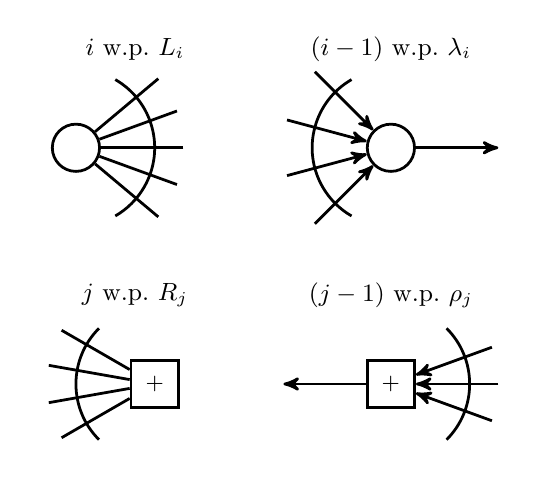
\begin{tikzpicture}
  [
  font=\small, line width=1pt, draw=black, >=stealth',
  bitnode/.style={circle, inner sep = 0pt, minimum size = 6mm, draw=black},
  checknode/.style={rectangle, inner sep = 0pt, minimum size = 6mm, draw=black},
  ]

  \node[bitnode] (L) at (0,3) {};
  \node[rotate around={-40:(L)}] (L0) at (1.5,3) {} edge (L);
  \node[rotate around={-20:(L)}] (L1) at (1.5,3) {} edge (L);
  \node[rotate around={0:(L)}] (L2) at (1.5,3) {} edge (L);
  \node[rotate around={20:(L)}] (L3) at (1.5,3) {} edge (L);
  \node[rotate around={40:(L)}] (L4) at (1.5,3) {} edge (L);
  \draw (L) ++(60:1) arc (60:-60:1);
  \node (Li) at (0.75,4.25) {$i$ w.p.\ $L_i$};

  \node[bitnode] (lambda) at (4,3) {};
  \node (lambda0) at (5.5,3) {} edge[<-] (lambda);
  \node[rotate around={-45:(lambda)}] (lambda1) at (2.5,3) {} edge[->] (lambda);
  \node[rotate around={-15:(lambda)}] (lambda2) at (2.5,3) {} edge[->] (lambda);
  \node[rotate around={15:(lambda)}] (lambda3) at (2.5,3) {} edge[->] (lambda);
  \node[rotate around={45:(lambda)}] (lambda4) at (2.5,3) {} edge[->] (lambda);
  \draw (lambda) ++(120:1) arc (120:240:1);
  \node (lambdai) at (4,4.25) {$(i-1)$ w.p.\ $\lambda_i$};
  
  \node[checknode] (R) at (1,0) {\footnotesize{$+$}};
  \node[rotate around={-30:(R)}] (R0) at (-0.5,0) {} edge (R);
  \node[rotate around={-10:(R)}] (R1) at (-0.5,0) {} edge (R);
  \node[rotate around={10:(R)}] (R2) at (-0.5,0) {} edge (R);
  \node[rotate around={30:(R)}] (R3) at (-0.5,0) {} edge (R);
  \draw (R) ++(135:1) arc (135:225:1);
  \node (Ri) at (0.75,1.125) {$j$ w.p.\ $R_j$};

  \node[checknode] (rho) at (4,0) {\footnotesize{$+$}};
  \node (R0) at (2.5,0) {} edge[<-] (rho);
  \node[rotate around={-20:(rho)}] (rho1) at (5.5,0) {} edge[->] (rho);
  \node (rho2) at (5.5,0) {} edge[->] (rho);
  \node[rotate around={20:(rho)}] (rho3) at (5.5,0) {} edge[->] (rho);
  \draw (rho) ++(45:1) arc (45:-45:1);
  \node (rhoi) at (4,1.125) {$(j-1)$ w.p.\ $\rho_j$};

\end{tikzpicture}
}
  \end{center}
\end{columns}
\footnotetext[1]{\scriptsize V. Zyablov, and M. Pinsker. ``Decoding complexity of low-density codes for transmission in a channel with erasures.'' Problemy Peredachi Informatsii (1974).}
\end{frame}


\begin{frame}{Computation Tree and Message Passing}
\begin{columns}
\column{.55\textwidth}
\begin{centering}
\scalebox{0.7}{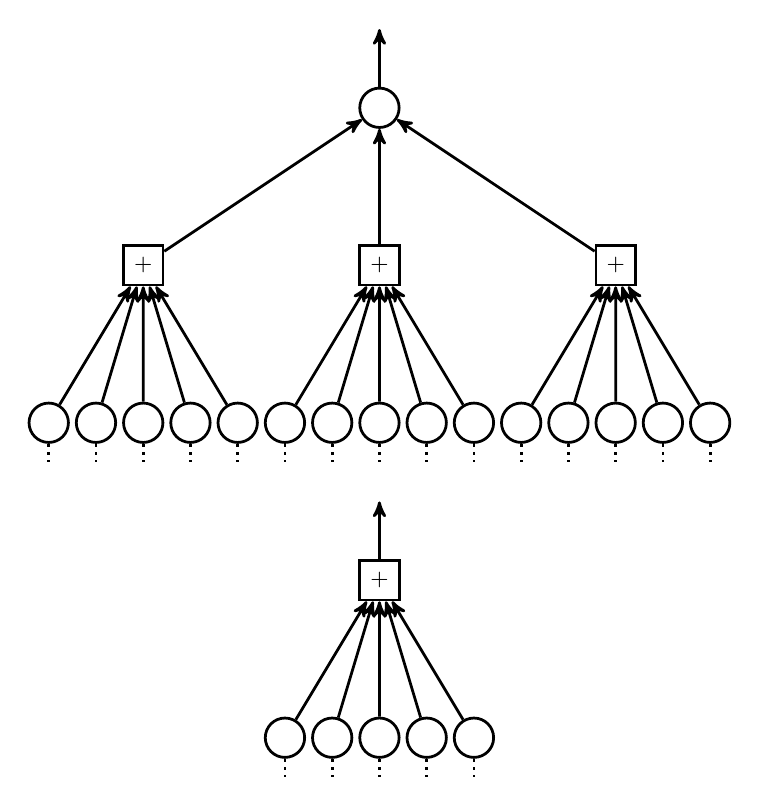
\begin{tikzpicture}
  [
  font=\small, line width=1pt, draw=black, >=stealth',
  bitnode/.style={circle, inner sep=0pt, minimum size=5mm, draw=black},
  checknode/.style={rectangle, inner sep=0pt, minimum size=5mm, draw=black},
  ]

  \node[bitnode] (b1) at (0,4) {}
    edge[->] (0,5);

  \foreach \x in {1,2,3} {
    \node[checknode] (c1\x) at (-6+3*\x,2) {\footnotesize{$+$}}
      edge[->] (b1);
  }

  \foreach \y in {1,2,3,4,5} {
    \node[bitnode] (b1\y) at (-4.8+0.6*\y,0) {}
      edge[->] (c11)
      edge[-,dotted] (-4.8+0.6*\y,-0.5);
    \node[bitnode] (b2\y) at (-1.8+0.6*\y,0) {}
      edge[->] (c12)
      edge[-,dotted] (-1.8+0.6*\y,-0.5);
    \node[bitnode] (b3\y) at (1.2+0.6*\y,0) {}
      edge[->] (c13)
      edge[-,dotted] (1.2+0.6*\y,-0.5);
  }
  
  \node[checknode] (c22) at (0,-2) {\footnotesize{$+$}}
    edge[->] (0,-1);

  \foreach \y in {1,2,3,4,5} {
    \node[bitnode] (b4\y) at (-1.8+0.6*\y,-4) {}
      edge[->] (c22)
      edge[-,dotted] (-1.8+0.6*\y,-4.5);
  }
\end{tikzpicture}

}
\end{centering}
\column{.4\textwidth}
\begin{block}{Standard Tricks}
\begin{itemize}
\item Unravel bipartite graph into computation graph
\item For large systems, graph is locally tree-like
\item Focus on outgoing messages
\item Analyze over random code ensemble
\end{itemize}
\end{block}
\end{columns}
\footnotetext[1]{\scriptsize M. Luby, M. Mitzenmacher, A. Shokrollahi, and D. Spielman. ``Efficient erasure correcting codes.'' IEEE Trans.\ on Information Theory (2001).}
\end{frame}


\begin{frame}
\frametitle{Graphical Methods: Tools from Iterative Decoding}
\begin{itemize}
\item $x$: Prob.\ outgoing message from variable node erased
\item $y$: Prob.\ outgoing message from check node erased
\end{itemize}
\begin{center}
\scalebox{0.7}{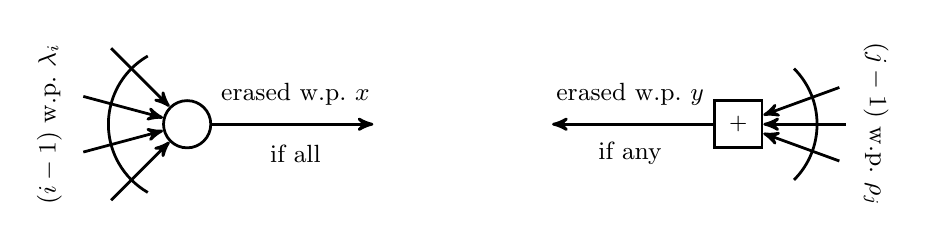
\begin{tikzpicture}
  [
  font=\small, line width=1pt, draw=black, >=stealth',
  bitnode/.style={circle, inner sep = 0pt, minimum size = 6mm, draw=black},
  checknode/.style={rectangle, inner sep = 0pt, minimum size = 6mm, draw=black},
  ]

  \node[bitnode] (lambda) at (0,0) {};
  \node (lambda0) at (2.5,0) {} edge[<-] (lambda);
  \node[rotate around={-45:(lambda)}] (lambda1) at (-1.5,0) {} edge[->] (lambda);
  \node[rotate around={-15:(lambda)}] (lambda2) at (-1.5,0) {} edge[->] (lambda);
  \node[rotate around={15:(lambda)}] (lambda3) at (-1.5,0) {} edge[->] (lambda);
  \node[rotate around={45:(lambda)}] (lambda4) at (-1.5,0) {} edge[->] (lambda);
  \draw (lambda) ++(120:1) arc (120:240:1);
  \node[rotate=90] (lambdai) at (-1.75,0) {$(i-1)$ w.p.\ $\lambda_i$};
  \node (x) at (1.375,0.375) {erased w.p.\ $x$};
  \node (x1) at (1.375,-0.375) {if all};
  
  \node[checknode] (rho) at (7,0) {\footnotesize{$+$}};
  \node (R0) at (4.5,0) {} edge[<-] (rho);
  \node[rotate around={-20:(rho)}] (rho1) at (8.5,0) {} edge[->] (rho);
  \node (rho2) at (8.5,0) {} edge[->] (rho);
  \node[rotate around={20:(rho)}] (rho3) at (8.5,0) {} edge[->] (rho);
  \draw (rho) ++(45:1) arc (45:-45:1);
  \node[rotate=-90] (rhoi) at (8.75,0) {$(j-1)$ w.p.\ $\rho_j$};
  \node (y) at (5.625,0.375) {erased w.p.\ $y$};
  \node (y1) at (5.625,-0.375) {if any};
\end{tikzpicture}
}
\end{center}
\begin{itemize}
\item Outgoing variable message is erased when all incoming check messages are erased
\begin{equation*}
x = \mathrm{E} \left[ y^{i-1} \right] = \lambda (y)
\end{equation*}
\item Outgoing check message is erased when one incoming variable message is erased
\begin{equation*}
y = \mathrm{E} \left[ 1 - (1 - x)^{j-1} \right] = 1 - \rho(1-x)
\end{equation*}
\end{itemize}
\end{frame}


\begin{frame}
\frametitle{Extrinsic Information Transfer (EXIT) Chart}
\begin{columns}
\column{.65\textwidth}
  \scalebox{0.85}{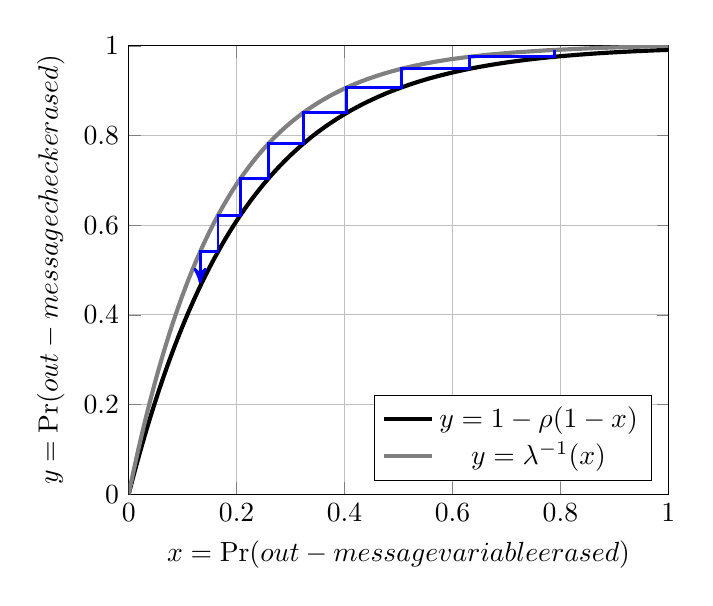
\begin{tikzpicture}
\begin{axis}[
  xlabel={$x = \Pr(\text{out-message variable erased})$},
  xmin=0, xmax=1,
  ymin=0, ymax=1,
  xmajorgrids,
  ylabel={$y = \Pr(\text{out-message check erased})$},
  legend pos=south east,
  ymajorgrids]

\addplot[color=black,line width=1.5pt]
coordinates{
(0.0000, 0.0000) (0.0050, 0.0232) (0.0100, 0.0459) (0.0150, 0.0681) (0.0200, 0.0898) (0.0250, 0.1109) (0.0300, 0.1316) (0.0350, 0.1518) (0.0400, 0.1715) (0.0450, 0.1907) (0.0500, 0.2095) (0.0550, 0.2279) (0.0600, 0.2458) (0.0650, 0.2634) (0.0700, 0.2805) (0.0750, 0.2972) (0.0800, 0.3135) (0.0850, 0.3295) (0.0900, 0.3451) (0.0950, 0.3603) (0.1000, 0.3751) (0.1050, 0.3897) (0.1100, 0.4039) (0.1150, 0.4177) (0.1200, 0.4312) (0.1250, 0.4445) (0.1300, 0.4574) (0.1350, 0.4700) (0.1400, 0.4823) (0.1450, 0.4943) (0.1500, 0.5061) (0.1550, 0.5175) (0.1600, 0.5288) (0.1650, 0.5397) (0.1700, 0.5504) (0.1750, 0.5609) (0.1800, 0.5711) (0.1850, 0.5810) (0.1900, 0.5908) (0.1950, 0.6003) (0.2000, 0.6096) (0.2050, 0.6186) (0.2100, 0.6275) (0.2150, 0.6362) (0.2200, 0.6446) (0.2250, 0.6529) (0.2300, 0.6609) (0.2350, 0.6688) (0.2400, 0.6765) (0.2450, 0.6840) (0.2500, 0.6914) (0.2550, 0.6985) (0.2600, 0.7055) (0.2650, 0.7124) (0.2700, 0.7191) (0.2750, 0.7256) (0.2800, 0.7320) (0.2850, 0.7382) (0.2900, 0.7443) (0.2950, 0.7502) (0.3000, 0.7560) (0.3050, 0.7617) (0.3100, 0.7672) (0.3150, 0.7726) (0.3200, 0.7779) (0.3250, 0.7831) (0.3300, 0.7881) (0.3350, 0.7931) (0.3400, 0.7979) (0.3450, 0.8026) (0.3500, 0.8072) (0.3550, 0.8116) (0.3600, 0.8160) (0.3650, 0.8203) (0.3700, 0.8245) (0.3750, 0.8285) (0.3800, 0.8325) (0.3850, 0.8364) (0.3900, 0.8402) (0.3950, 0.8439) (0.4000, 0.8476) (0.4050, 0.8511) (0.4100, 0.8546) (0.4150, 0.8579) (0.4200, 0.8612) (0.4250, 0.8645) (0.4300, 0.8676) (0.4350, 0.8707) (0.4400, 0.8737) (0.4450, 0.8766) (0.4500, 0.8795) (0.4550, 0.8823) (0.4600, 0.8850) (0.4650, 0.8877) (0.4700, 0.8903) (0.4750, 0.8929) (0.4800, 0.8954) (0.4850, 0.8978) (0.4900, 0.9002) (0.4950, 0.9025) (0.5000, 0.9047) (0.5050, 0.9070) (0.5100, 0.9091) (0.5150, 0.9112) (0.5200, 0.9133) (0.5250, 0.9153) (0.5300, 0.9173) (0.5350, 0.9192) (0.5400, 0.9211) (0.5450, 0.9229) (0.5500, 0.9247) (0.5550, 0.9265) (0.5600, 0.9282) (0.5650, 0.9298) (0.5700, 0.9315) (0.5750, 0.9331) (0.5800, 0.9346) (0.5850, 0.9361) (0.5900, 0.9376) (0.5950, 0.9391) (0.6000, 0.9405) (0.6050, 0.9419) (0.6100, 0.9432) (0.6150, 0.9445) (0.6200, 0.9458) (0.6250, 0.9471) (0.6300, 0.9483) (0.6350, 0.9495) (0.6400, 0.9507) (0.6450, 0.9518) (0.6500, 0.9530) (0.6550, 0.9540) (0.6600, 0.9551) (0.6650, 0.9562) (0.6700, 0.9572) (0.6750, 0.9582) (0.6800, 0.9591) (0.6850, 0.9601) (0.6900, 0.9610) (0.6950, 0.9619) (0.7000, 0.9628) (0.7050, 0.9637) (0.7100, 0.9645) (0.7150, 0.9653) (0.7200, 0.9661) (0.7250, 0.9669) (0.7300, 0.9677) (0.7350, 0.9685) (0.7400, 0.9692) (0.7450, 0.9699) (0.7500, 0.9706) (0.7550, 0.9713) (0.7600, 0.9720) (0.7650, 0.9726) (0.7700, 0.9732) (0.7750, 0.9739) (0.7800, 0.9745) (0.7850, 0.9751) (0.7900, 0.9756) (0.7950, 0.9762) (0.8000, 0.9768) (0.8050, 0.9773) (0.8100, 0.9778) (0.8150, 0.9783) (0.8200, 0.9788) (0.8250, 0.9793) (0.8300, 0.9798) (0.8350, 0.9803) (0.8400, 0.9807) (0.8450, 0.9812) (0.8500, 0.9816) (0.8550, 0.9821) (0.8600, 0.9825) (0.8650, 0.9829) (0.8700, 0.9833) (0.8750, 0.9837) (0.8800, 0.9840) (0.8850, 0.9844) (0.8900, 0.9848) (0.8950, 0.9851) (0.9000, 0.9855) (0.9050, 0.9858) (0.9100, 0.9861) (0.9150, 0.9865) (0.9200, 0.9868) (0.9250, 0.9871) (0.9300, 0.9874) (0.9350, 0.9877) (0.9400, 0.9880) (0.9450, 0.9882) (0.9500, 0.9885) (0.9550, 0.9888) (0.9600, 0.9890) (0.9650, 0.9893) (0.9700, 0.9896) (0.9750, 0.9898) (0.9800, 0.9900) (0.9850, 0.9903) (0.9900, 0.9905) (0.9950, 0.9907) (1.0000, 0.9909)
};
\addlegendentry{$y = 1 - \rho (1 - x)$}

\addplot[color=gray,line width=1.5pt]
coordinates{
(0.0000, 0.0000) (0.0009, 0.0050) (0.0017, 0.0100) (0.0026, 0.0150) (0.0034, 0.0200) (0.0043, 0.0250) (0.0052, 0.0300) (0.0061, 0.0350) (0.0069, 0.0400) (0.0078, 0.0450) (0.0087, 0.0500) (0.0096, 0.0550) (0.0105, 0.0600) (0.0114, 0.0650) (0.0123, 0.0700) (0.0133, 0.0750) (0.0142, 0.0800) (0.0151, 0.0850) (0.0160, 0.0900) (0.0170, 0.0950) (0.0179, 0.1000) (0.0189, 0.1050) (0.0198, 0.1100) (0.0208, 0.1150) (0.0217, 0.1200) (0.0227, 0.1250) (0.0237, 0.1300) (0.0247, 0.1350) (0.0257, 0.1400) (0.0267, 0.1450) (0.0276, 0.1500) (0.0287, 0.1550) (0.0297, 0.1600) (0.0307, 0.1650) (0.0317, 0.1700) (0.0327, 0.1750) (0.0338, 0.1800) (0.0348, 0.1850) (0.0358, 0.1900) (0.0369, 0.1950) (0.0380, 0.2000) (0.0390, 0.2050) (0.0401, 0.2100) (0.0412, 0.2150) (0.0423, 0.2200) (0.0434, 0.2250) (0.0445, 0.2300) (0.0456, 0.2350) (0.0467, 0.2400) (0.0478, 0.2450) (0.0489, 0.2500) (0.0501, 0.2550) (0.0512, 0.2600) (0.0524, 0.2650) (0.0535, 0.2700) (0.0547, 0.2750) (0.0559, 0.2800) (0.0571, 0.2850) (0.0583, 0.2900) (0.0595, 0.2950) (0.0607, 0.3000) (0.0619, 0.3050) (0.0631, 0.3100) (0.0644, 0.3150) (0.0656, 0.3200) (0.0669, 0.3250) (0.0681, 0.3300) (0.0694, 0.3350) (0.0707, 0.3400) (0.0720, 0.3450) (0.0733, 0.3500) (0.0746, 0.3550) (0.0759, 0.3600) (0.0773, 0.3650) (0.0786, 0.3700) (0.0800, 0.3750) (0.0813, 0.3800) (0.0827, 0.3850) (0.0841, 0.3900) (0.0855, 0.3950) (0.0869, 0.4000) (0.0883, 0.4050) (0.0898, 0.4100) (0.0912, 0.4150) (0.0927, 0.4200) (0.0941, 0.4250) (0.0956, 0.4300) (0.0971, 0.4350) (0.0986, 0.4400) (0.1002, 0.4450) (0.1017, 0.4500) (0.1033, 0.4550) (0.1048, 0.4600) (0.1064, 0.4650) (0.1080, 0.4700) (0.1096, 0.4750) (0.1112, 0.4800) (0.1129, 0.4850) (0.1146, 0.4900) (0.1162, 0.4950) (0.1179, 0.5000) (0.1196, 0.5050) (0.1214, 0.5100) (0.1231, 0.5150) (0.1249, 0.5200) (0.1266, 0.5250) (0.1284, 0.5300) (0.1303, 0.5350) (0.1321, 0.5400) (0.1340, 0.5450) (0.1358, 0.5500) (0.1377, 0.5550) (0.1397, 0.5600) (0.1416, 0.5650) (0.1436, 0.5700) (0.1456, 0.5750) (0.1476, 0.5800) (0.1496, 0.5850) (0.1517, 0.5900) (0.1538, 0.5950) (0.1559, 0.6000) (0.1580, 0.6050) (0.1602, 0.6100) (0.1624, 0.6150) (0.1646, 0.6200) (0.1669, 0.6250) (0.1691, 0.6300) (0.1715, 0.6350) (0.1738, 0.6400) (0.1762, 0.6450) (0.1786, 0.6500) (0.1810, 0.6550) (0.1835, 0.6600) (0.1861, 0.6650) (0.1886, 0.6700) (0.1912, 0.6750) (0.1938, 0.6800) (0.1965, 0.6850) (0.1992, 0.6900) (0.2020, 0.6950) (0.2048, 0.7000) (0.2077, 0.7050) (0.2106, 0.7100) (0.2136, 0.7150) (0.2166, 0.7200) (0.2196, 0.7250) (0.2228, 0.7300) (0.2259, 0.7350) (0.2292, 0.7400) (0.2325, 0.7450) (0.2358, 0.7500) (0.2393, 0.7550) (0.2428, 0.7600) (0.2464, 0.7650) (0.2500, 0.7700) (0.2538, 0.7750) (0.2576, 0.7800) (0.2615, 0.7850) (0.2655, 0.7900) (0.2696, 0.7950) (0.2738, 0.8000) (0.2781, 0.8050) (0.2825, 0.8100) (0.2871, 0.8150) (0.2917, 0.8200) (0.2965, 0.8250) (0.3015, 0.8300) (0.3065, 0.8350) (0.3118, 0.8400) (0.3172, 0.8450) (0.3227, 0.8500) (0.3285, 0.8550) (0.3345, 0.8600) (0.3407, 0.8650) (0.3471, 0.8700) (0.3538, 0.8750) (0.3607, 0.8800) (0.3680, 0.8850) (0.3755, 0.8900) (0.3834, 0.8950) (0.3917, 0.9000) (0.4005, 0.9050) (0.4097, 0.9100) (0.4194, 0.9150) (0.4297, 0.9200) (0.4407, 0.9250) (0.4524, 0.9300) (0.4650, 0.9350) (0.4786, 0.9400) (0.4934, 0.9450) (0.5096, 0.9500) (0.5276, 0.9550) (0.5476, 0.9600) (0.5703, 0.9650) (0.5965, 0.9700) (0.6274, 0.9750) (0.6649, 0.9800) (0.7123, 0.9850) (0.7753, 0.9900) (0.8644, 0.9950) (1.0000, 1.0000)
};
\addlegendentry{$y = \lambda^{-1}(x)$}

\addplot[color=blue,line width=1pt,->,>=stealth']
coordinates{
(0.7894, 0.9909) (0.7894, 0.9756) (0.6313, 0.9756) (0.6313, 0.9486) (0.5051, 0.9486) (0.5051, 0.9070) (0.4040, 0.9070) (0.4040, 0.8504) (0.3232, 0.8504) (0.3232, 0.7813) (0.2586, 0.7813) (0.2586, 0.7036) (0.2069, 0.7036) (0.2069, 0.6220) (0.1655, 0.6220) (0.1655, 0.5408) (0.1324, 0.5408)
(0.1324, 0.47)
};
\end{axis}
\end{tikzpicture}
}
\column{.3\textwidth}
  \scalebox{0.85}{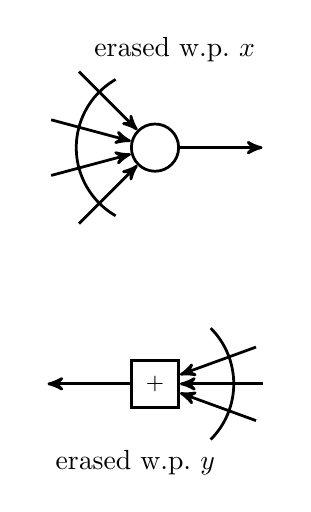
\begin{tikzpicture}
  [
  %font=\small,
  line width=1pt,
  draw=black, >=stealth',
  bitnode/.style={circle, inner sep = 0pt, minimum size = 6mm, draw=black},
  checknode/.style={rectangle, inner sep = 0pt, minimum size = 6mm, draw=black},
  ]

  \node[bitnode] (lambda) at (0,3) {};
  \node (lambda0) at (1.5,3) {} edge[<-] (lambda);
  \node[rotate around={-45:(lambda)}] (lambda1) at (-1.5,3) {} edge[->] (lambda);
  \node[rotate around={-15:(lambda)}] (lambda2) at (-1.5,3) {} edge[->] (lambda);
  \node[rotate around={15:(lambda)}] (lambda3) at (-1.5,3) {} edge[->] (lambda);
  \node[rotate around={45:(lambda)}] (lambda4) at (-1.5,3) {} edge[->] (lambda);
  \draw (lambda) ++(120:1) arc (120:240:1);
  \node (x) at (0.25,4.25) {erased w.p.\ $x$};
  
  \node[checknode] (rho) at (0,0) {\footnotesize{$+$}};
  \node (R0) at (-1.5,0) {} edge[<-] (rho);
  \node[rotate around={-20:(rho)}] (rho1) at (1.5,0) {} edge[->] (rho);
  \node (rho2) at (1.5,0) {} edge[->] (rho);
  \node[rotate around={20:(rho)}] (rho3) at (1.5,0) {} edge[->] (rho);
  \draw (rho) ++(45:1) arc (45:-45:1);
  \node (x) at (-0.25,-1) {erased w.p.\ $y$};
\end{tikzpicture}

}
\end{columns}
\vfill
\textbf{Step-by-Step Progression}
\begin{xalignat*}{2}
y &= 1 - \rho(1-x) &
x &= \lambda(y) \quad \text{ \textcolor{gray}{(flipped)}}
\end{xalignat*}
\end{frame}


\begin{frame}
\frametitle{Example -- Traditional Fountain Codes}
\begin{columns}
\column{.48\textwidth}
\begin{center}
  \scalebox{0.55}{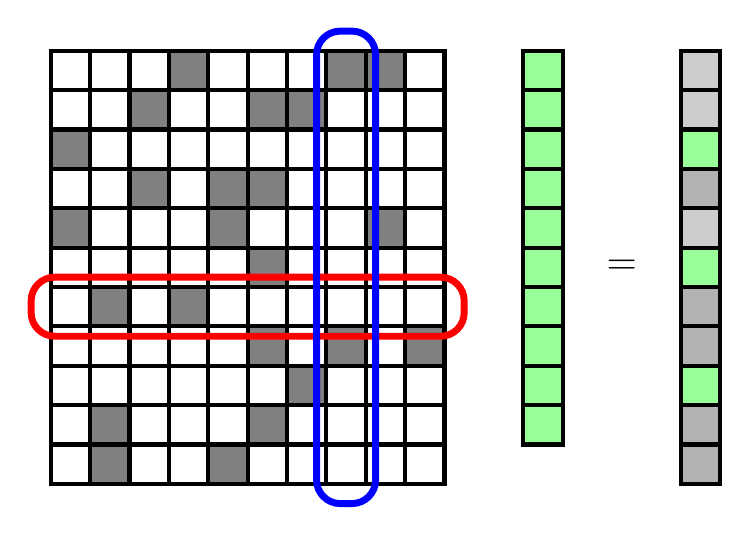
\begin{tikzpicture}
[draw=black, line width=1.5pt, >=stealth',
entry1/.style={rectangle, draw, fill=gray, inner sep=0pt, minimum size=5mm},
entry0/.style={rectangle, draw, inner sep=0pt, minimum size=5mm},
symbol/.style={rectangle, draw, fill=green!40, inner sep=0pt, minimum size=5mm}]

\node[entry0] (m00) at (0,0) {};
\node[entry1] (m01) at (0.5,0) {};
\node[entry0] (m02) at (1,0) {};
\node[entry0] (m03) at (1.5,0) {};
\node[entry1] (m04) at (2,0) {};
\node[entry0] (m05) at (2.5,0) {};
\node[entry0] (m06) at (3,0) {};
\node[entry0] (m07) at (3.5,0) {};
\node[entry0] (m08) at (4,0) {};
\node[entry0] (m09) at (4.5,0) {};

\node[entry0] (m00) at (0,0.5) {};
\node[entry1] (m11) at (0.5,0.5) {};
\node[entry0] (m12) at (1,0.5) {};
\node[entry0] (m13) at (1.5,0.5) {};
\node[entry0] (m14) at (2,0.5) {};
\node[entry1] (m15) at (2.5,0.5) {};
\node[entry0] (m16) at (3,0.5) {};
\node[entry0] (m17) at (3.5,0.5) {};
\node[entry0] (m18) at (4,0.5) {};
\node[entry0] (m19) at (4.5,0.5) {};

\node[entry0] (m20) at (0,1) {};
\node[entry0] (m21) at (0.5,1) {};
\node[entry0] (m22) at (1,1) {};
\node[entry0] (m23) at (1.5,1) {};
\node[entry0] (m24) at (2,1) {};
\node[entry0] (m25) at (2.5,1) {};
\node[entry1] (m26) at (3,1) {};
\node[entry0] (m27) at (3.5,1) {};
\node[entry0] (m28) at (4,1) {};
\node[entry0] (m29) at (4.5,1) {};

\node[entry0] (m30) at (0,1.5) {};
\node[entry0] (m31) at (0.5,1.5) {};
\node[entry0] (m32) at (1,1.5) {};
\node[entry0] (m33) at (1.5,1.5) {};
\node[entry0] (m34) at (2,1.5) {};
\node[entry1] (m35) at (2.5,1.5) {};
\node[entry0] (m36) at (3,1.5) {};
\node[entry1] (m37) at (3.5,1.5) {};
\node[entry0] (m38) at (4,1.5) {};
\node[entry1] (m39) at (4.5,1.5) {};

\node[entry0] (m40) at (0,2) {};
\node[entry1] (m41) at (0.5,2) {};
\node[entry0] (m42) at (1,2) {};
\node[entry1] (m43) at (1.5,2) {};
\node[entry0] (m44) at (2,2) {};
\node[entry0] (m45) at (2.5,2) {};
\node[entry0] (m46) at (3,2) {};
\node[entry0] (m47) at (3.5,2) {};
\node[entry0] (m48) at (4,2) {};
\node[entry0] (m49) at (4.5,2) {};

\node[entry0] (m50) at (0,2.5) {};
\node[entry0] (m51) at (0.5,2.5) {};
\node[entry0] (m52) at (1,2.5) {};
\node[entry0] (m53) at (1.5,2.5) {};
\node[entry0] (m54) at (2,2.5) {};
\node[entry1] (m55) at (2.5,2.5) {};
\node[entry0] (m56) at (3,2.5) {};
\node[entry0] (m57) at (3.5,2.5) {};
\node[entry0] (m58) at (4,2.5) {};
\node[entry0] (m59) at (4.5,2.5) {};

\node[entry1] (m60) at (0,3) {};
\node[entry0] (m61) at (0.5,3) {};
\node[entry0] (m62) at (1,3) {};
\node[entry0] (m63) at (1.5,3) {};
\node[entry1] (m64) at (2,3) {};
\node[entry0] (m65) at (2.5,3) {};
\node[entry0] (m66) at (3,3) {};
\node[entry0] (m67) at (3.5,3) {};
\node[entry1] (m68) at (4,3) {};
\node[entry0] (m69) at (4.5,3) {};

\node[entry0] (m70) at (0,3.5) {};
\node[entry0] (m71) at (0.5,3.5) {};
\node[entry1] (m72) at (1,3.5) {};
\node[entry0] (m73) at (1.5,3.5) {};
\node[entry1] (m74) at (2,3.5) {};
\node[entry1] (m75) at (2.5,3.5) {};
\node[entry0] (m76) at (3,3.5) {};
\node[entry0] (m77) at (3.5,3.5) {};
\node[entry0] (m78) at (4,3.5) {};
\node[entry0] (m79) at (4.5,3.5) {};

\node[entry1] (m80) at (0,4) {};
\node[entry0] (m81) at (0.5,4) {};
\node[entry0] (m82) at (1,4) {};
\node[entry0] (m83) at (1.5,4) {};
\node[entry0] (m84) at (2,4) {};
\node[entry0] (m85) at (2.5,4) {};
\node[entry0] (m86) at (3,4) {};
\node[entry0] (m87) at (3.5,4) {};
\node[entry0] (m88) at (4,4) {};
\node[entry0] (m89) at (4.5,4) {};

\node[entry0] (m90) at (0,4.5) {};
\node[entry0] (m91) at (0.5,4.5) {};
\node[entry1] (m92) at (1,4.5) {};
\node[entry0] (m93) at (1.5,4.5) {};
\node[entry0] (m94) at (2,4.5) {};
\node[entry1] (m95) at (2.5,4.5) {};
\node[entry1] (m96) at (3,4.5) {};
\node[entry0] (m97) at (3.5,4.5) {};
\node[entry0] (m98) at (4,4.5) {};
\node[entry0] (m99) at (4.5,4.5) {};

\node[entry0] (m100) at (0,5) {};
\node[entry0] (m101) at (0.5,5) {};
\node[entry0] (m102) at (1,5) {};
\node[entry1] (m103) at (1.5,5) {};
\node[entry0] (m104) at (2,5) {};
\node[entry0] (m105) at (2.5,5) {};
\node[entry0] (m106) at (3,5) {};
\node[entry1] (m107) at (3.5,5) {};
\node[entry1] (m108) at (4,5) {};
\node[entry0] (m109) at (4.5,5) {};


\node[symbol] (s1) at (6,0.5) {};
\node[symbol] (s2) at (6,1) {};
\node[symbol] (s3) at (6,1.5) {};
\node[symbol] (s4) at (6,2) {};
\node[symbol] (s5) at (6,2.5) {};
\node[symbol] (s6) at (6,3) {};
\node[symbol] (s7) at (6,3.5) {};
\node[symbol] (s8) at (6,4) {};
\node[symbol] (s9) at (6,4.5) {};
\node[symbol] (s10) at (6,5) {};

\node (equal) at (7,2.5) {\Large =};

\node[entry0,fill=black!30] (y0) at (8,0) {};
\node[entry0,fill=black!30] (y1) at (8,0.5) {};
\node[symbol] (y2) at (8,1) {};
\node[entry0,fill=black!30] (y3) at (8,1.5) {};
\node[entry0,fill=black!30] (y4) at (8,2) {};
\node[symbol] (y5) at (8,2.5) {};
\node[entry0,fill=black!20] (y6) at (8,3) {};
\node[entry0,fill=black!30] (y7) at (8,3.5) {};
\node[symbol] (y8) at (8,4) {};
\node[entry0,fill=black!20] (y9) at (8,4.5) {};
\node[entry0,fill=black!20] (y10) at (8,5) {};

\draw[draw=red,line width=2.5pt,rounded corners=3mm] (-0.5,1.625) rectangle (5,2.375);
\draw[draw=blue,line width=2.5pt,rounded corners=3mm] (3.125,-0.5) rectangle (3.875,5.5);

\end{tikzpicture}

}
\end{center}
\column{.5\textwidth}
\begin{itemize}
\item Select \# of bit nodes
\item Pick bits uniformly
\item Columns not selected independently
\item Cannot be employed in massive uncoordinated multiple access
\end{itemize}
\end{columns}
\begin{center}
  \scalebox{0.8}{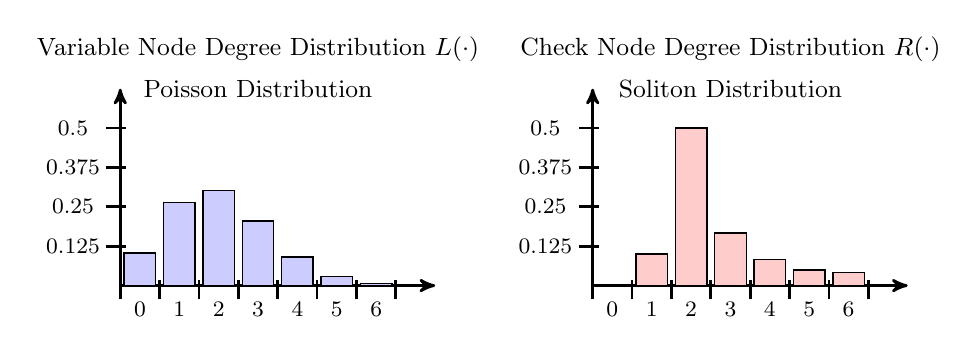
\begin{tikzpicture}[
  font=\footnotesize,
  >=stealth',
  line width=1pt,
]

\draw [<->] (0,2.5) -- (0,0) -- (4,0);
\foreach \x in {0,...,7} {
  \draw (0.5*\x,-0.175) -- (0.5*\x,0.075);
}
\foreach \x in {0,1,...,6} {
  \node (tx\x) at (0.5*\x+0.25,-0.3) {\x};
}
\foreach \x in {1,...,4} {
  \draw (-0.175,0.5*\x) -- (0.075,0.5*\x);
}
\node (ty0) at (1.75,3) {\small Variable Node Degree Distribution $L(\cdot)$};
\node (ty00) at (1.75,2.5) {\small Poisson Distribution};
\node (ty1) at (-0.6,0.5) {0.125};
\node (ty2) at (-0.6,1) {0.25};
\node (ty3) at (-0.6,1.5) {0.375};
\node (ty4) at (-0.6,2) {0.5};
\draw[fill=blue!20,line width=0.5pt] (0.05,0) rectangle (0.45,0.414);
\draw[fill=blue!20,line width=0.5pt] (0.55,0) rectangle (0.95,1.054);
\draw[fill=blue!20,line width=0.5pt] (1.05,0) rectangle (1.45,1.208);
\draw[fill=blue!20,line width=0.5pt] (1.55,0) rectangle (1.95,0.820);
\draw[fill=blue!20,line width=0.5pt] (2.05,0) rectangle (2.45,0.365);
\draw[fill=blue!20,line width=0.5pt] (2.55,0) rectangle (2.95,0.112);
\draw[fill=blue!20,line width=0.5pt] (3.05,0) rectangle (3.45,0.024);

\draw [<->] (6,2.5) -- (6,0) -- (10,0);
\foreach \x in {0,...,7} {
  \draw (0.5*\x+6,-0.175) -- (0.5*\x+6,0.075);
}
\foreach \x in {0,1,...,6} {
  \node (txx\x) at (0.5*\x+6.25,-0.3) {\x};
}
\foreach \x in {1,...,4} {
  \draw (6-0.175,0.5*\x) -- (6.075,0.5*\x);
}
\node (tyy0) at (7.75,3) {\small Check Node Degree Distribution $R(\cdot)$};
\node (tyy00) at (7.75,2.5) {\small Soliton Distribution};
\node (tyy1) at (6-0.6,0.5) {0.125};
\node (tyy2) at (6-0.6,1) {0.25};
\node (tyy3) at (6-0.6,1.5) {0.375};
\node (tyy4) at (6-0.6,2) {0.5};
\draw[fill=red!20,line width=0.5pt] (6.55,0) rectangle (6.95,4/10);
\draw[fill=red!20,line width=0.5pt] (7.05,0) rectangle (7.45,4/2);
\draw[fill=red!20,line width=0.5pt] (7.55,0) rectangle (7.95,4/6);
\draw[fill=red!20,line width=0.5pt] (8.05,0) rectangle (8.45,4/12);
\draw[fill=red!20,line width=0.5pt] (8.55,0) rectangle (8.95,4/20);
\draw[fill=red!20,line width=0.5pt] (9.05,0) rectangle (9.45,4/24);
\end{tikzpicture}

}
\end{center}
\footnotetext[1]{K. Narayanan and H. Pfister. ``Iterative collision resolution for slotted ALOHA: An optimal uncoordinated transmission policy.'' ISTC, 2012.}
\end{frame}


\begin{frame}
\frametitle{Example -- Transpose of LT Codes}
\begin{columns}
\column{.48\textwidth}
\begin{center}
  \scalebox{0.55}{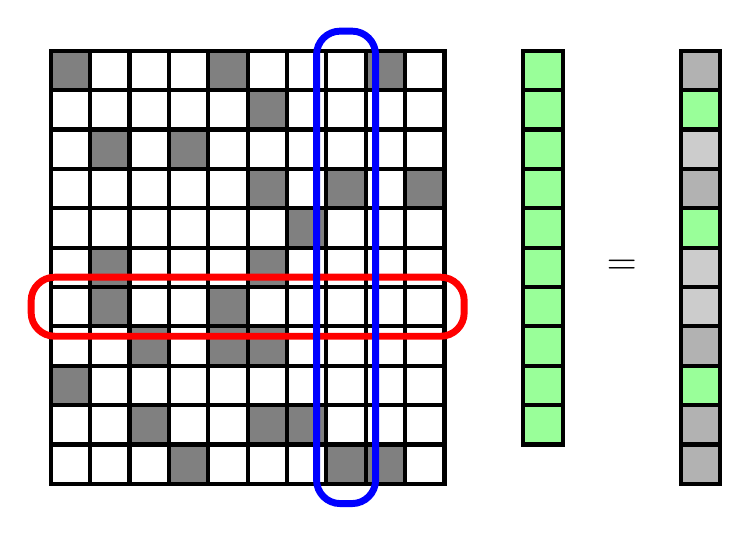
\begin{tikzpicture}
[draw=black, line width=1.5pt, >=stealth',
entry1/.style={rectangle, draw, fill=gray, inner sep=0pt, minimum size=5mm},
entry0/.style={rectangle, draw, inner sep=0pt, minimum size=5mm},
symbol/.style={rectangle, draw, fill=green!40, inner sep=0pt, minimum size=5mm}]

\node[entry0] (m00) at (0,0) {};
\node[entry0] (m01) at (0.5,0) {};
\node[entry0] (m02) at (1,0) {};
\node[entry1] (m03) at (1.5,0) {};
\node[entry0] (m04) at (2,0) {};
\node[entry0] (m05) at (2.5,0) {};
\node[entry0] (m06) at (3,0) {};
\node[entry1] (m07) at (3.5,0) {};
\node[entry1] (m08) at (4,0) {};
\node[entry0] (m09) at (4.5,0) {};

\node[entry0] (m00) at (0,0.5) {};
\node[entry0] (m11) at (0.5,0.5) {};
\node[entry1] (m12) at (1,0.5) {};
\node[entry0] (m13) at (1.5,0.5) {};
\node[entry0] (m14) at (2,0.5) {};
\node[entry1] (m15) at (2.5,0.5) {};
\node[entry1] (m16) at (3,0.5) {};
\node[entry0] (m17) at (3.5,0.5) {};
\node[entry0] (m18) at (4,0.5) {};
\node[entry0] (m19) at (4.5,0.5) {};

\node[entry1] (m20) at (0,1) {};
\node[entry0] (m21) at (0.5,1) {};
\node[entry0] (m22) at (1,1) {};
\node[entry0] (m23) at (1.5,1) {};
\node[entry0] (m24) at (2,1) {};
\node[entry0] (m25) at (2.5,1) {};
\node[entry0] (m26) at (3,1) {};
\node[entry0] (m27) at (3.5,1) {};
\node[entry0] (m28) at (4,1) {};
\node[entry0] (m29) at (4.5,1) {};

\node[entry0] (m30) at (0,1.5) {};
\node[entry0] (m31) at (0.5,1.5) {};
\node[entry1] (m32) at (1,1.5) {};
\node[entry0] (m33) at (1.5,1.5) {};
\node[entry1] (m34) at (2,1.5) {};
\node[entry1] (m35) at (2.5,1.5) {};
\node[entry0] (m36) at (3,1.5) {};
\node[entry0] (m37) at (3.5,1.5) {};
\node[entry0] (m38) at (4,1.5) {};
\node[entry0] (m39) at (4.5,1.5) {};

\node[entry0] (m40) at (0,2) {};
\node[entry1] (m41) at (0.5,2) {};
\node[entry0] (m42) at (1,2) {};
\node[entry0] (m43) at (1.5,2) {};
\node[entry1] (m44) at (2,2) {};
\node[entry0] (m45) at (2.5,2) {};
\node[entry0] (m46) at (3,2) {};
\node[entry0] (m47) at (3.5,2) {};
\node[entry0] (m48) at (4,2) {};
\node[entry0] (m49) at (4.5,2) {};

\node[entry0] (m50) at (0,2.5) {};
\node[entry1] (m51) at (0.5,2.5) {};
\node[entry0] (m52) at (1,2.5) {};
\node[entry0] (m53) at (1.5,2.5) {};
\node[entry0] (m54) at (2,2.5) {};
\node[entry1] (m55) at (2.5,2.5) {};
\node[entry0] (m56) at (3,2.5) {};
\node[entry0] (m57) at (3.5,2.5) {};
\node[entry0] (m58) at (4,2.5) {};
\node[entry0] (m59) at (4.5,2.5) {};

\node[entry0] (m60) at (0,3) {};
\node[entry0] (m61) at (0.5,3) {};
\node[entry0] (m62) at (1,3) {};
\node[entry0] (m63) at (1.5,3) {};
\node[entry0] (m64) at (2,3) {};
\node[entry0] (m65) at (2.5,3) {};
\node[entry1] (m66) at (3,3) {};
\node[entry0] (m67) at (3.5,3) {};
\node[entry0] (m68) at (4,3) {};
\node[entry0] (m69) at (4.5,3) {};

\node[entry0] (m70) at (0,3.5) {};
\node[entry0] (m71) at (0.5,3.5) {};
\node[entry0] (m72) at (1,3.5) {};
\node[entry0] (m73) at (1.5,3.5) {};
\node[entry0] (m74) at (2,3.5) {};
\node[entry1] (m75) at (2.5,3.5) {};
\node[entry0] (m76) at (3,3.5) {};
\node[entry1] (m77) at (3.5,3.5) {};
\node[entry0] (m78) at (4,3.5) {};
\node[entry1] (m79) at (4.5,3.5) {};

\node[entry0] (m80) at (0,4) {};
\node[entry1] (m81) at (0.5,4) {};
\node[entry0] (m82) at (1,4) {};
\node[entry1] (m83) at (1.5,4) {};
\node[entry0] (m84) at (2,4) {};
\node[entry0] (m85) at (2.5,4) {};
\node[entry0] (m86) at (3,4) {};
\node[entry0] (m87) at (3.5,4) {};
\node[entry0] (m88) at (4,4) {};
\node[entry0] (m89) at (4.5,4) {};

\node[entry0] (m90) at (0,4.5) {};
\node[entry0] (m91) at (0.5,4.5) {};
\node[entry0] (m92) at (1,4.5) {};
\node[entry0] (m93) at (1.5,4.5) {};
\node[entry0] (m94) at (2,4.5) {};
\node[entry1] (m95) at (2.5,4.5) {};
\node[entry0] (m96) at (3,4.5) {};
\node[entry0] (m97) at (3.5,4.5) {};
\node[entry0] (m98) at (4,4.5) {};
\node[entry0] (m99) at (4.5,4.5) {};

\node[entry1] (m100) at (0,5) {};
\node[entry0] (m101) at (0.5,5) {};
\node[entry0] (m102) at (1,5) {};
\node[entry0] (m103) at (1.5,5) {};
\node[entry1] (m104) at (2,5) {};
\node[entry0] (m105) at (2.5,5) {};
\node[entry0] (m106) at (3,5) {};
\node[entry0] (m107) at (3.5,5) {};
\node[entry1] (m108) at (4,5) {};
\node[entry0] (m109) at (4.5,5) {};


\node[symbol] (s1) at (6,0.5) {};
\node[symbol] (s2) at (6,1) {};
\node[symbol] (s3) at (6,1.5) {};
\node[symbol] (s4) at (6,2) {};
\node[symbol] (s5) at (6,2.5) {};
\node[symbol] (s6) at (6,3) {};
\node[symbol] (s7) at (6,3.5) {};
\node[symbol] (s8) at (6,4) {};
\node[symbol] (s9) at (6,4.5) {};
\node[symbol] (s10) at (6,5) {};

\node (equal) at (7,2.5) {\Large =};

\node[entry0,fill=black!30] (y0) at (8,0) {};
\node[entry0,fill=black!30] (y1) at (8,0.5) {};
\node[symbol] (y2) at (8,1) {};
\node[entry0,fill=black!30] (y3) at (8,1.5) {};
\node[entry0,fill=black!20] (y4) at (8,2) {};
\node[entry0,fill=black!20] (y5) at (8,2.5) {};
\node[symbol] (y6) at (8,3) {};
\node[entry0,fill=black!30] (y7) at (8,3.5) {};
\node[entry0,fill=black!20] (y8) at (8,4) {};
\node[entry0,symbol] (y9) at (8,4.5) {};
\node[entry0,fill=black!30] (y10) at (8,5) {};

\draw[draw=red,line width=2.5pt,rounded corners=3mm] (-0.5,1.625) rectangle (5,2.375);
\draw[draw=blue,line width=2.5pt,rounded corners=3mm] (3.125,-0.5) rectangle (3.875,5.5);

\end{tikzpicture}

}
\end{center}
\column{.5\textwidth}
\begin{itemize}
\item Devices pick \# of transmissions
\item Selects slots uniformly
\item Columns are independently
\item Admissible massive uncoordinated multiple access
\end{itemize}
\end{columns}
\begin{center}
  \scalebox{0.8}{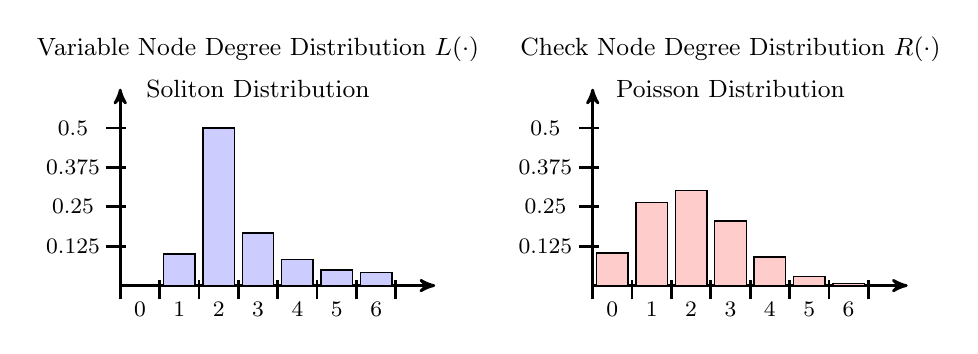
\begin{tikzpicture}[
  font=\footnotesize,
  >=stealth',
  line width=1pt,
]

\draw [<->] (0,2.5) -- (0,0) -- (4,0);
\foreach \x in {0,...,7} {
  \draw (0.5*\x,-0.175) -- (0.5*\x,0.075);
}
\foreach \x in {0,1,...,6} {
  \node (tx\x) at (0.5*\x+0.25,-0.3) {\x};
}
\foreach \x in {1,...,4} {
  \draw (-0.175,0.5*\x) -- (0.075,0.5*\x);
}
\node (ty0) at (1.75,3) {\small Variable Node Degree Distribution $L(\cdot)$};
\node (ty00) at (1.75,2.5) {\small Soliton Distribution};
\node (ty1) at (-0.6,0.5) {0.125};
\node (ty2) at (-0.6,1) {0.25};
\node (ty3) at (-0.6,1.5) {0.375};
\node (ty4) at (-0.6,2) {0.5};
\draw[fill=blue!20,line width=0.5pt] (0.55,0) rectangle (0.95,4/10);
\draw[fill=blue!20,line width=0.5pt] (1.05,0) rectangle (1.45,4/2);
\draw[fill=blue!20,line width=0.5pt] (1.55,0) rectangle (1.95,4/6);
\draw[fill=blue!20,line width=0.5pt] (2.05,0) rectangle (2.45,4/12);
\draw[fill=blue!20,line width=0.5pt] (2.55,0) rectangle (2.95,4/20);
\draw[fill=blue!20,line width=0.5pt] (3.05,0) rectangle (3.45,4/24);

\draw [<->] (6,2.5) -- (6,0) -- (10,0);
\foreach \x in {0,...,7} {
  \draw (0.5*\x+6,-0.175) -- (0.5*\x+6,0.075);
}
\foreach \x in {0,1,...,6} {
  \node (txx\x) at (0.5*\x+6.25,-0.3) {\x};
}
\foreach \x in {1,...,4} {
  \draw (6-0.175,0.5*\x) -- (6.075,0.5*\x);
}
\node (tyy0) at (7.75,3) {\small Check Node Degree Distribution $R(\cdot)$};
\node (ty00) at (7.75,2.5) {\small Poisson Distribution};
\node (tyy1) at (6-0.6,0.5) {0.125};
\node (tyy2) at (6-0.6,1) {0.25};
\node (tyy3) at (6-0.6,1.5) {0.375};
\node (tyy4) at (6-0.6,2) {0.5};
\draw[fill=red!20,line width=0.5pt] (6.05,0) rectangle (6.45,0.414);
\draw[fill=red!20,line width=0.5pt] (6.55,0) rectangle (6.95,1.054);
\draw[fill=red!20,line width=0.5pt] (7.05,0) rectangle (7.45,1.208);
\draw[fill=red!20,line width=0.5pt] (7.55,0) rectangle (7.95,0.820);
\draw[fill=red!20,line width=0.5pt] (8.05,0) rectangle (8.45,0.365);
\draw[fill=red!20,line width=0.5pt] (8.55,0) rectangle (8.95,0.112);
\draw[fill=red!20,line width=0.5pt] (9.05,0) rectangle (9.45,0.024);
\end{tikzpicture}

}
\end{center}
\footnotetext[1]{K. Narayanan and H. Pfister. ``Iterative collision resolution for slotted ALOHA: An optimal uncoordinated transmission policy.'' ISTC, 2012.}
\end{frame}


\begin{frame}
\frametitle{Optimal Scheme when Number of Devices Known}
\begin{center}
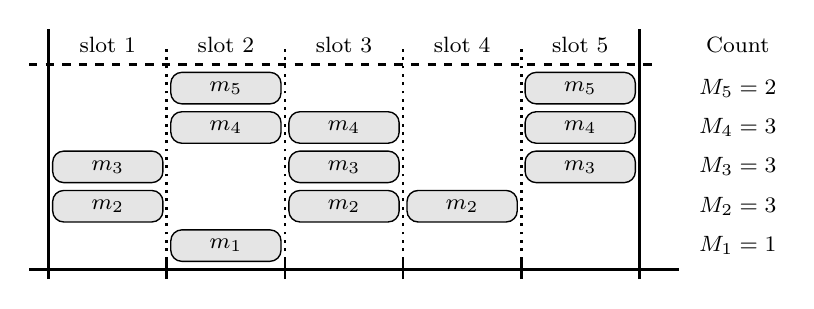
\begin{tikzpicture}[
  font=\footnotesize,
  >=stealth',
  line width=1pt,
  device/.style={circle, inner sep = 0pt, minimum height=3mm, minimum width=3mm, draw=black, fill=gray!40, line width=0.5pt},
  slot/.style={circle, inner sep = 0pt, minimum height=1.5mm, fill=black, line width=0.5pt},
  packet/.style={rectangle, minimum height=4mm, minimum width=14mm, draw=black, fill=gray!20, rounded corners, line width=0.5pt}
]

\draw (0,-0.05) -- (8.25,-0.05);
\draw (0.25,-0.175) -- (0.25,3.0);
\foreach \x in {1,...,4} {
  \draw (1.5*\x+0.25,-0.175) -- (1.5*\x+0.25,0.075);
  \draw[dotted] (1.5*\x+0.25,0.075) -- (1.5*\x+0.25,2.8);
}
\draw (7.75,-0.175) -- (7.75,3.0);
\draw[dashed] (0,2.55) -- (8,2.55);

\foreach \x in {1,...,5} {
  \node (t\x) at (1.5*\x-0.5,2.8) {slot~\x};
}

\node (count) at (9,2.8) {Count};
\node (M1) at (9.0,0.25) {$M_1 = 1$};
\node (M2) at (9.0,0.75) {$M_2 = 3$};
\node (M3) at (9.0,1.25) {$M_3 = 3$};
\node (M4) at (9.0,1.75) {$M_4 = 3$};
\node (M5) at (9.0,2.25) {$M_5 = 2$};

\node[packet] (p12) at (2.5,0.25) {$m_1$};
\node[packet] (p21) at (1.0,0.75) {$m_2$};
\node[packet] (p23) at (4.0,0.75) {$m_2$};
\node[packet] (p24) at (5.5,0.75) {$m_2$};
\node[packet] (p31) at (1.0,1.25) {$m_3$};
\node[packet] (p33) at (4.0,1.25) {$m_3$};
\node[packet] (p35) at (7.0,1.25) {$m_3$};
\node[packet] (p42) at (2.5,1.75) {$m_4$};
\node[packet] (p43) at (4.0,1.75) {$m_4$};
\node[packet] (p45) at (7.0,1.75) {$m_4$};
\node[packet] (p52) at (2.5,2.25) {$m_5$};
\node[packet] (p55) at (7.0,2.25) {$m_5$};

\end{tikzpicture}


\end{center}
\begin{itemize}
\item Every device picks random slot count according to Soliton
  \begin{equation*}
  p_{\mathrm{sol}(t)}(m)
  = \begin{cases}
  {1}/{t} & m = 1 \\
  {1}/{((m-1)m)} & m = 2, \ldots t
  \end{cases}
  \end{equation*}
\item Given count, select $m$ slots uniformly at random
\item Induce Soliton on left and Poisson on right of Tanner graph
\item Asymptotically \textbf{optimal} when number of devices is known
\end{itemize}
\end{frame}


\begin{frame}
\frametitle{Proof Sketch -- Access with Dual Fountain Codes}
\begin{columns}
\column{.40\textwidth}
\begin{block}{LT Codes}
\begin{itemize}
\item Degree distributions
\begin{gather*}
L(\cdot) \text{ Poisson dist}\\
R(\cdot) \text{ Soliton dist}
\end{gather*}
\item Fountain codes optimal (asymptotically)
\begin{align*}
\lambda(z) = e^{- r_{\mathrm{avg}}(1-z)} \\
\rho(z) = - \ln (1-z)
\end{align*}
\item Density evolution
\begin{align*}
y &= 1 - \rho(1-x) \\
x &= \lambda(y)
\end{align*}
%\item Original LT Recursions
%\begin{align*}
%y_{t+1} &= 1 - \rho(1 - \lambda(y_t)) \rightarrow 0 \\
%x_{t+1} &= \lambda(1 - \rho(1 - x_t)) \rightarrow 0
%\end{align*}
\end{itemize}
\end{block}
\column{.55\textwidth}
\begin{block}{Uncoordinated MAC}
\begin{itemize}
\item Degree distributions
\begin{gather*}
\tilde{L}(\cdot) = R(\cdot) \text{ Soliton dist}\\
\tilde{R}(\cdot) = L(\cdot) \text{ Poisson dist}
\end{gather*}
\item Density evolution
\begin{align*}
y %&= 1 - \tilde{\rho}(1-x) \\
%&= 1 - \lambda(1-x) \\
&= 1 - e^{- r_{\mathrm{avg}}x} \\
x %&= \tilde{\lambda}(y)
%= \rho(y)
&= - \ln (1-y)
\end{align*}
\item Recursions
\begin{equation*}
\begin{split}
y_{t+1} %&= 1 - \lambda(1 - \rho(y_t)) \\
&= 1 - e^{ r_{\mathrm{avg}} \ln (1-y)} \\
&= 1 - (1-y)^{r_{\mathrm{avg}}}
\end{split}
\end{equation*}
\end{itemize}
\end{block}
\end{columns}
\centerline{Throughput $\rightarrow 1$ when $K$ known}
\end{frame}


\begin{frame}
\frametitle{Revised System Assumptions}
\begin{itemize}
\item Devices operate with \textbf{no side information}, $K$ unknown
\item Access point broadcasts start/end of every round
\item Joint decoding via successive interference cancellation: \textbf{peeling} algorithm
\end{itemize}
\begin{block}{Other Considerations}
\begin{itemize}
\item \textbf{Slots per round} can differ based on number of devices
\item Perhaps length of round  can be determined dynamically?
\end{itemize}
\begin{center}
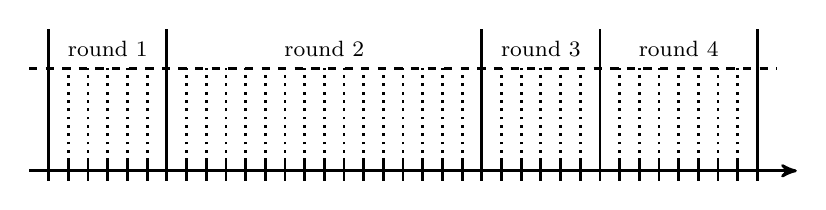
\begin{tikzpicture}[
  font=\footnotesize,
  >=stealth',
  line width=1pt
]

\draw [->] (0,-0.05) -- (9.75,-0.05);
\foreach \x in {0,...,36} {
  \draw (0.25*\x+0.25,-0.175) -- (0.25*\x+0.25,0.075);
  \draw[dotted] (0.25*\x+0.25,0.075) -- (0.25*\x+0.25,1.25);
}
\draw (0.25,-0.175) -- (0.25,1.75);
\draw (1.75,-0.175) -- (1.75,1.75);
\draw (5.75,-0.175) -- (5.75,1.75);
\draw (7.25,-0.175) -- (7.25,1.75);
\draw (9.25,-0.175) -- (9.25,1.75);
\draw[dashed] (0,1.25) -- (9.5,1.25);

\node (t1) at (1,1.5) {round~1};
\node (t1) at (3.75,1.5) {round~2};
\node (t1) at (6.5,1.5) {round~3};
\node (t1) at (8.25,1.5) {round~4};

\end{tikzpicture}


\end{center}
\end{block}
\end{frame}


\begin{frame}
\frametitle{Universality}
\begin{itemize}
	\item Previous frameworks require the number of users to be known
		\begin{itemize}
			\item to determine the round duration
			\item or to determine the slot access probability (Frameless ALOHA)
		\end{itemize}
\vspace{3mm}

	\item<2-> \textbf{Number of active devices} may be \textbf{unknown} a priori
	\item<2-> Access point may not need to know beforehand!

\vspace{3mm}
	\item<3-> Joint Estimation and Contention-Resolution-STPP'13\footnotemark
		\begin{itemize}
			\item<3-> Joint estimation of number of users and resolution of user packets
			\item<3-> Multiple rounds, estimate of number of users is improved each round
			\item<3-> Dynamic round durations as a function of fraction of users resolved
		\end{itemize}
\end{itemize}

\vspace{3mm}
\only<4->{\textit{Our framework is universal: Does not require number of users to be known or estimated}}

\only<3->{\footnotetext[1]{\scriptsize{[STPP'13] \v{C}. Stefanovi\'{c}, K. F. Trilingsgaard, N. K. Pratas,  P. Popovski, ``Joint Estimation and Contention-Resolution Protocol for Wireless Random Access'', IEEE ICC 2013.}}}
\end{frame}


\begin{frame}
\frametitle{Soliton Distribution when Number of Devices Unknown}
  \begin{center}
  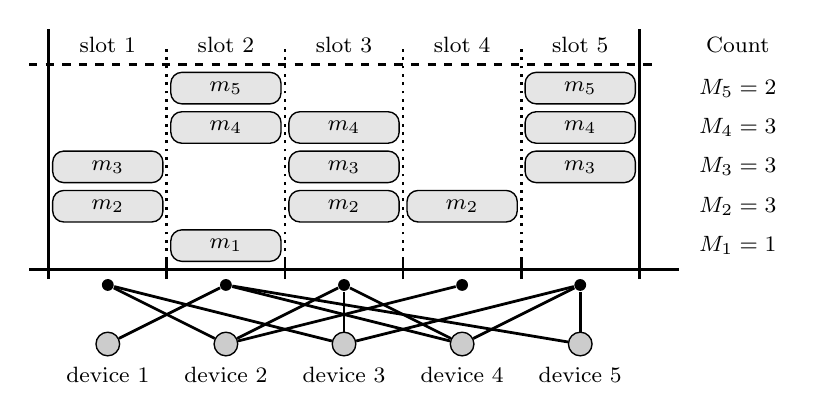
\begin{tikzpicture}[
  font=\footnotesize,
  >=stealth',
  line width=1pt,
  device/.style={circle, inner sep = 0pt, minimum height=3mm, minimum width=3mm, draw=black, fill=gray!40, line width=0.5pt},
  slot/.style={circle, inner sep = 0pt, minimum height=1.5mm, fill=black, line width=0.5pt},
  packet/.style={rectangle, minimum height=4mm, minimum width=14mm, draw=black, fill=gray!20, rounded corners, line width=0.5pt}
]

\draw (0,-0.05) -- (8.25,-0.05);
\draw (0.25,-0.175) -- (0.25,3.0);
\foreach \x in {1,...,4} {
  \draw (1.5*\x+0.25,-0.175) -- (1.5*\x+0.25,0.075);
  \draw[dotted] (1.5*\x+0.25,0.075) -- (1.5*\x+0.25,2.8);
}
\draw (7.75,-0.175) -- (7.75,3.0);
\draw[dashed] (0,2.55) -- (8,2.55);

\foreach \x in {1,...,5} {
  \node[slot] (s\x) at (1.5*\x-0.5,-0.25) {};
  \node (t\x) at (1.5*\x-0.5,2.8) {slot~\x};
}

\node (count) at (9,2.8) {Count};
\node (M1) at (9.0,0.25) {$M_1 = 1$};
\node (M2) at (9.0,0.75) {$M_2 = 3$};
\node (M3) at (9.0,1.25) {$M_3 = 3$};
\node (M4) at (9.0,1.75) {$M_4 = 3$};
\node (M5) at (9.0,2.25) {$M_5 = 2$};

\node[device] (d1) at (1,-1) [label=below:device~1]{};
\node[device] (d2) at (2.5,-1) [label=below:device~2]{};
\node[device] (d3) at (4,-1) [label=below:device~3]{};
\node[device] (d4) at (5.5,-1) [label=below:device~4]{};
\node[device] (d5) at (7.0,-1) [label=below:device~5]{};

\draw (d1) -- (s2);
\draw (d2) -- (s1);
\draw (d2) -- (s3);
\draw (d2) -- (s4);
\draw (d3) -- (s1);
\draw (d3) -- (s3);
\draw (d3) -- (s5);
\draw (d4) -- (s2);
\draw (d4) -- (s3);
\draw (d4) -- (s5);
\draw (d5) -- (s2);
\draw (d5) -- (s5);

\node[packet] (p12) at (2.5,0.25) {$m_1$};
\node[packet] (p21) at (1.0,0.75) {$m_2$};
\node[packet] (p23) at (4.0,0.75) {$m_2$};
\node[packet] (p24) at (5.5,0.75) {$m_2$};
\node[packet] (p31) at (1.0,1.25) {$m_3$};
\node[packet] (p33) at (4.0,1.25) {$m_3$};
\node[packet] (p35) at (7.0,1.25) {$m_3$};
\node[packet] (p42) at (2.5,1.75) {$m_4$};
\node[packet] (p43) at (4.0,1.75) {$m_4$};
\node[packet] (p45) at (7.0,1.75) {$m_4$};
\node[packet] (p52) at (2.5,2.25) {$m_5$};
\node[packet] (p55) at (7.0,2.25) {$m_5$};

\end{tikzpicture}


  \end{center}
  \begin{itemize}
  \item When number of active devices is $t$, we want round to end after approximately $t$ slots
  \item \textbf{First Guess:} When number of device is $t$, random slot count for each device at end time~$t$ should have Soliton distribution $p_{\mathrm{sol}(t)}(\cdot)$, independent of one another
  \end{itemize}
\end{frame}


\begin{frame}
\frametitle{Challenge in Designing Universal Schemes}
\begin{block}{Challenge}
\begin{itemize}
\item If device operates in isolation, it does not know total number of active devices nor slot count for current round
\item Yet, packet count should have Soliton distribution $p_{\mathrm{sol}(s)}(\cdot)$ at end of round
\item  One way to fulfill requirement is for rolling message count to possess Soliton distribution $p_{\mathrm{sol}(s)}(\cdot)$ at every time~$s$
\end{itemize}
\end{block}
\begin{center}
\textbf{Can this be achieved?}
\end{center}
\end{frame}


\begin{frame}
\frametitle{Potential Solution -- Time-Varying Markov Chain}
\begin{center}
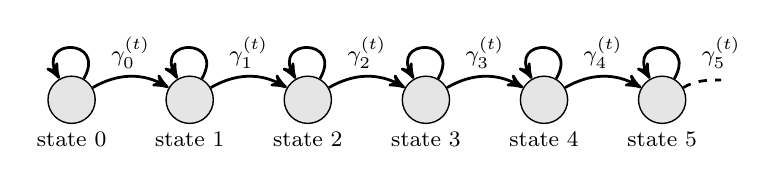
\begin{tikzpicture}[
  font=\footnotesize,
  >=stealth',
  line width=1pt,
  state/.style={circle, draw=black, inner sep = 0pt, minimum size = 6mm, draw=black, fill=gray!20, line width=0.5pt}]

\foreach \x in {0,...,5} {
  \node[state] (s\x) at (1.5*\x,0) {};
  \node (t\x) at (1.5*\x,-0.5) {state~\x};
}

\draw [->] (s0) to [out=60, in=120, looseness=5] (s0);
\draw [->] (s1) to [out=60, in=120, looseness=5] (s1);
\draw [->] (s2) to [out=60, in=120, looseness=5] (s2);
\draw [->] (s3) to [out=60, in=120, looseness=5] (s3);
\draw [->] (s4) to [out=60, in=120, looseness=5] (s4);
\draw [->] (s5) to [out=60, in=120, looseness=5] (s5);

\draw [->] (s0) to [out=30, in=150, looseness=1] (s1);
\draw [->] (s1) to [out=30, in=150, looseness=1] (s2);
\draw [->] (s2) to [out=30, in=150, looseness=1] (s3);
\draw [->] (s3) to [out=30, in=150, looseness=1] (s4);
\draw [->] (s4) to [out=30, in=150, looseness=1] (s5);
\draw [dashed] (s5) to [out=30, in=180, looseness=1] (8.25,0.25);

\node (g0) at (0.75,0.6) {$\gamma_0^{(t)}$};
\node (g1) at (2.25,0.6) {$\gamma_1^{(t)}$};
\node (g2) at (3.75,0.6) {$\gamma_2^{(t)}$};
\node (g3) at (5.25,0.6) {$\gamma_3^{(t)}$};
\node (g4) at (6.75,0.6) {$\gamma_4^{(t)}$};
\node (g5) at (8.25,0.6) {$\gamma_5^{(t)}$};

\end{tikzpicture}


\end{center}
\begin{itemize}
\item Every device contains state machine initialized to 0 at onset of round
\item Device transmits a copy of message whenever Markov chain jumps to right neighbor
\item State denotes number of copies transmitted thus far
\item Transition probabilities are time varying
\item Progression of Markov chain independent from one device to another
%\item Chain is semi-infinite to accommodate round of any size
\end{itemize}
\end{frame}


\begin{frame}
\frametitle{Computing Transition Probabilities}
\begin{center}
\scalebox{0.9}{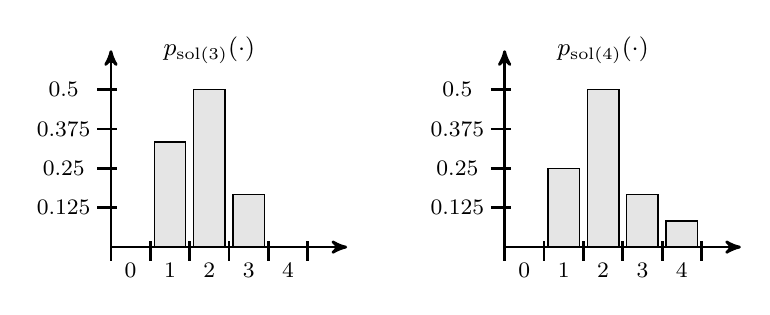
\begin{tikzpicture}[
  font=\footnotesize,
  >=stealth',
  line width=1pt,
]

\draw [<->] (0,2.5) -- (0,0) -- (3,0);
\foreach \x in {0,...,5} {
  \draw (0.5*\x,-0.175) -- (0.5*\x,0.075);
}
\foreach \x in {0,1,...,4} {
  \node (tx\x) at (0.5*\x+0.25,-0.3) {\x};
}
\foreach \x in {1,...,4} {
  \draw (-0.175,0.5*\x) -- (0.075,0.5*\x);
}
\node (ty1) at (1.25,2.5) {\small $p_{\mathrm{sol}(3)}(\cdot)$};
\node (ty1) at (-0.6,0.5) {0.125};
\node (ty2) at (-0.6,1) {0.25};
\node (ty3) at (-0.6,1.5) {0.375};
\node (ty4) at (-0.6,2) {0.5};
\draw[fill=gray!20,line width=0.5pt] (0.55,0) rectangle (0.95,4/3);
\draw[fill=gray!20,line width=0.5pt] (1.05,0) rectangle (1.45,4/2);
\draw[fill=gray!20,line width=0.5pt] (1.55,0) rectangle (1.95,4/6);


\draw [<->] (5,2.5) -- (5,0) -- (8,0);
\foreach \x in {0,...,5} {
  \draw (0.5*\x+5,-0.175) -- (0.5*\x+5,0.075);
}
\foreach \x in {0,1,...,4} {
  \node (txx\x) at (0.5*\x+5.25,-0.3) {\x};
}
\foreach \x in {1,...,4} {
  \draw (5-0.175,0.5*\x) -- (5.075,0.5*\x);
}
\node (tyy1) at (6.25,2.5) {\small $p_{\mathrm{sol}(4)}(\cdot)$};
\node (tyy1) at (5-0.6,0.5) {0.125};
\node (tyy2) at (5-0.6,1) {0.25};
\node (tyy3) at (5-0.6,1.5) {0.375};
\node (tyy4) at (5-0.6,2) {0.5};
\draw[fill=gray!20,line width=0.5pt] (5.55,0) rectangle (5.95,4/4);
\draw[fill=gray!20,line width=0.5pt] (6.05,0) rectangle (6.45,4/2);
\draw[fill=gray!20,line width=0.5pt] (6.55,0) rectangle (6.95,4/6);
\draw[fill=gray!20,line width=0.5pt] (7.05,0) rectangle (7.45,4/12);

\end{tikzpicture}
}
\end{center}
\begin{itemize}
\item Must find transition probabilities to shift from $p_{\mathrm{sol}(3)}(\cdot)$ to $p_{\mathrm{sol}(4)}(\cdot)$
\end{itemize}
\begin{center}
\scalebox{0.9}{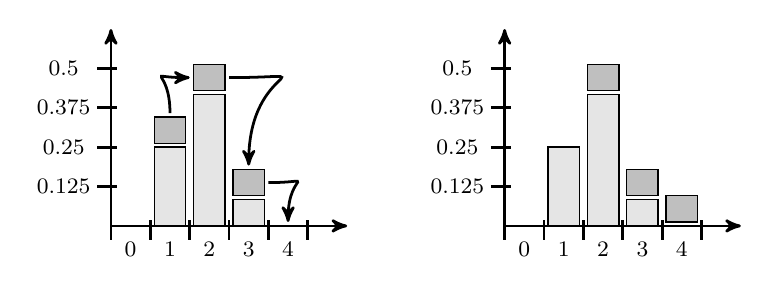
\begin{tikzpicture}[
  font=\footnotesize,
  >=stealth',
  line width=1pt,
]

\draw [<->] (0,2.5) -- (0,0) -- (3,0);
\foreach \x in {0,...,5} {
  \draw (0.5*\x,-0.175) -- (0.5*\x,0.075);
}
\foreach \x in {0,1,...,4} {
  \node (tx\x) at (0.5*\x+0.25,-0.3) {\x};
}
\foreach \x in {1,...,4} {
  \draw (-0.175,0.5*\x) -- (0.075,0.5*\x);
}
\node (ty1) at (-0.6,0.5) {0.125};
\node (ty2) at (-0.6,1) {0.25};
\node (ty3) at (-0.6,1.5) {0.375};
\node (ty4) at (-0.6,2) {0.5};
\draw[fill=gray!20,line width=0.5pt] (0.55,0) rectangle (0.95,1);
\draw[fill=gray!50,line width=0.5pt] (0.55,1+0.05) rectangle (0.95,4/3+0.05);
\draw[fill=gray!20,line width=0.5pt] (1.05,0) rectangle (1.45,5/3);
\draw[fill=gray!50,line width=0.5pt] (1.05,5/3+0.05) rectangle (1.45,2+0.05);
\draw[fill=gray!20,line width=0.5pt] (1.55,0) rectangle (1.95,1/3);
\draw[fill=gray!50,line width=0.5pt] (1.55,1/3+0.05) rectangle (1.95,2/3+0.05);

\draw [->] (0.75,4/3+0.1) to [out=90, in=180, looseness=3] (1.,11/6+0.05);
\draw [->] (1.5,11/6+0.05) to [out=0, in=90, looseness=3] (1.75,2/3+0.1);
\draw [->] (2,1/2+0.05) to [out=0, in=90, looseness=3] (2.25,0.05);


\draw [<->] (5,2.5) -- (5,0) -- (8,0);
\foreach \x in {0,...,5} {
  \draw (0.5*\x+5,-0.175) -- (0.5*\x+5,0.075);
}
\foreach \x in {0,1,...,4} {
  \node (txx\x) at (0.5*\x+5.25,-0.3) {\x};
}
\foreach \x in {1,...,4} {
  \draw (5-0.175,0.5*\x) -- (5.075,0.5*\x);
}
\node (tyy1) at (5-0.6,0.5) {0.125};
\node (tyy2) at (5-0.6,1) {0.25};
\node (tyy3) at (5-0.6,1.5) {0.375};
\node (tyy4) at (5-0.6,2) {0.5};
\draw[fill=gray!20,line width=0.5pt] (5.55,0) rectangle (5.95,1);
\draw[fill=gray!20,line width=0.5pt] (6.05,0) rectangle (6.45,5/3);
\draw[fill=gray!50,line width=0.5pt] (6.05,5/3+0.05) rectangle (6.45,2+0.05);
\draw[fill=gray!20,line width=0.5pt] (6.55,0) rectangle (6.95,1/3);
\draw[fill=gray!50,line width=0.5pt] (6.55,1/3+0.05) rectangle (6.95,2/3+0.05);
\draw[fill=gray!50,line width=0.5pt] (7.05,0.05) rectangle (7.45,1/3+0.05);

\end{tikzpicture}
}
\end{center}
\end{frame}


\begin{frame}
\frametitle{Shifting from One Distribution to Another}
\begin{center}
\scalebox{0.9}{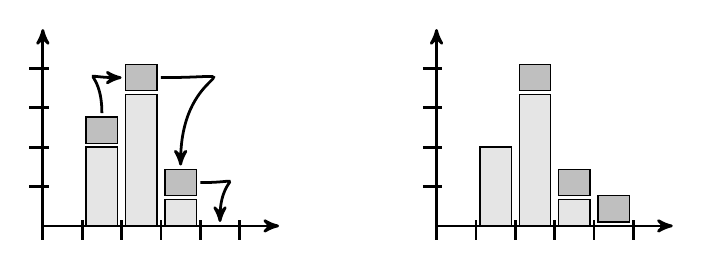
\begin{tikzpicture}[
  font=\footnotesize,
  >=stealth',
  line width=1pt,
]

\draw [<->] (0,2.5) -- (0,0) -- (3,0);
\foreach \x in {0,...,5} {
  \draw (0.5*\x,-0.175) -- (0.5*\x,0.075);
}
\foreach \x in {1,...,4} {
  \draw (-0.175,0.5*\x) -- (0.075,0.5*\x);
}
\draw[fill=gray!20,line width=0.5pt] (0.55,0) rectangle (0.95,1);
\draw[fill=gray!50,line width=0.5pt] (0.55,1+0.05) rectangle (0.95,4/3+0.05);
\draw[fill=gray!20,line width=0.5pt] (1.05,0) rectangle (1.45,5/3);
\draw[fill=gray!50,line width=0.5pt] (1.05,5/3+0.05) rectangle (1.45,2+0.05);
\draw[fill=gray!20,line width=0.5pt] (1.55,0) rectangle (1.95,1/3);
\draw[fill=gray!50,line width=0.5pt] (1.55,1/3+0.05) rectangle (1.95,2/3+0.05);

\draw [->] (0.75,4/3+0.1) to [out=90, in=180, looseness=3] (1.,11/6+0.05);
\draw [->] (1.5,11/6+0.05) to [out=0, in=90, looseness=3] (1.75,2/3+0.1);
\draw [->] (2,1/2+0.05) to [out=0, in=90, looseness=3] (2.25,0.05);


\draw [<->] (5,2.5) -- (5,0) -- (8,0);
\foreach \x in {0,...,5} {
  \draw (0.5*\x+5,-0.175) -- (0.5*\x+5,0.075);
}
\foreach \x in {1,...,4} {
  \draw (5-0.175,0.5*\x) -- (5.075,0.5*\x);
}
\draw[fill=gray!20,line width=0.5pt] (5.55,0) rectangle (5.95,1);
\draw[fill=gray!20,line width=0.5pt] (6.05,0) rectangle (6.45,5/3);
\draw[fill=gray!50,line width=0.5pt] (6.05,5/3+0.05) rectangle (6.45,2+0.05);
\draw[fill=gray!20,line width=0.5pt] (6.55,0) rectangle (6.95,1/3);
\draw[fill=gray!50,line width=0.5pt] (6.55,1/3+0.05) rectangle (6.95,2/3+0.05);
\draw[fill=gray!50,line width=0.5pt] (7.05,0.05) rectangle (7.45,1/3+0.05);

\end{tikzpicture}
}
\end{center}
\begin{enumerate}
\item Condition~1: Need enough probability mass to push over to neighbor
\item Condition~2: Can't push probability mass past immediate neighbor
\item Conditions can be expressed mathematically in terms of first-order stochastic dominance
\begin{equation*}
X \preceq Y \text{ whenever }
\Pr (X > m) \leq \Pr (Y > m) \quad \forall m
\end{equation*}
or, equivalently, cumulative distribution function (CDF) of $X$ dominates CDF of $Y$
\end{enumerate}
\end{frame}


\begin{frame}
\frametitle{Markov Chains and Distribution Shaping}
\begin{itemize}
\item Let $p_0(\cdot), p_1(\cdot), p_2(\cdot), \ldots$ be a sequence of probability distributions
\item Let $S$ denote standard right shift operator acting on one-sided infinite sequences
\end{itemize}
\begin{center}
 \scalebox{0.9}{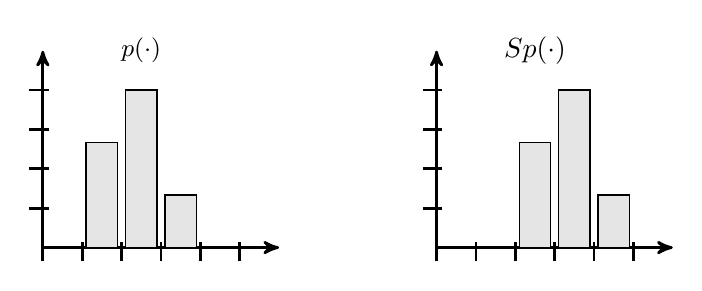
\begin{tikzpicture}[
  >=stealth',
  line width=1pt,
]

\draw [<->] (0,2.5) -- (0,0) -- (3,0);
\foreach \x in {0,...,5} {
  \draw (0.5*\x,-0.175) -- (0.5*\x,0.075);
}
\foreach \x in {1,...,4} {
  \draw (-0.175,0.5*\x) -- (0.075,0.5*\x);
}
\node (ty1) at (1.25,2.5) {\small $p(\cdot)$};
\draw[fill=gray!20,line width=0.5pt] (0.55,0) rectangle (0.95,4/3);
\draw[fill=gray!20,line width=0.5pt] (1.05,0) rectangle (1.45,4/2);
\draw[fill=gray!20,line width=0.5pt] (1.55,0) rectangle (1.95,4/6);


\draw [<->] (5,2.5) -- (5,0) -- (8,0);
\foreach \x in {0,...,5} {
  \draw (0.5*\x+5,-0.175) -- (0.5*\x+5,0.075);
}
\foreach \x in {1,...,4} {
  \draw (5-0.175,0.5*\x) -- (5.075,0.5*\x);
}
\node (tyy1) at (6.25,2.5) {$S p(\cdot)$};
\draw[fill=gray!20,line width=0.5pt] (6.05,0) rectangle (6.45,4/3);
\draw[fill=gray!20,line width=0.5pt] (6.55,0) rectangle (6.95,4/2);
\draw[fill=gray!20,line width=0.5pt] (7.05,0) rectangle (7.45,4/6);

\end{tikzpicture}
}
\end{center}
\textbf{Theorem:}
Sequence of distributions can be achieved through monotone increasing Markov chain with self-transitions and transitions to nearest neighbors on the right iff
\begin{itemize}
\item $p_t \preceq p_{t+1}$ for every $t$ \textcolor{gray}{-- enough probability mass to push to right}
\item $p_{t+1} \preceq S p_t$ for every $t$ \textcolor{gray}{-- cannot push mass past the neighbor}
\end{itemize}
\end{frame}


\begin{frame}
\frametitle{Applying Markov Shaping Strategy}
\begin{center}
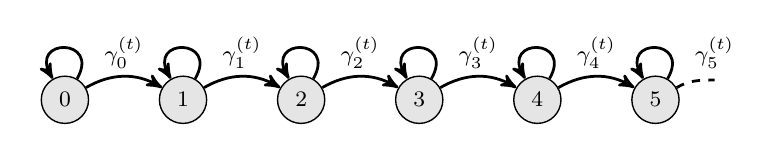
\begin{tikzpicture}[
  font=\footnotesize,
  >=stealth',
  line width=1pt,
  state/.style={circle, draw=black, inner sep = 0pt, minimum size = 6mm, draw=black, fill=gray!20, line width=0.5pt}]

\foreach \x in {0,...,5} {
  \node[state] (s\x) at (1.5*\x,0) {\x};
}

\draw [->] (s0) to [out=60, in=120, looseness=5] (s0);
\draw [->] (s1) to [out=60, in=120, looseness=5] (s1);
\draw [->] (s2) to [out=60, in=120, looseness=5] (s2);
\draw [->] (s3) to [out=60, in=120, looseness=5] (s3);
\draw [->] (s4) to [out=60, in=120, looseness=5] (s4);
\draw [->] (s5) to [out=60, in=120, looseness=5] (s5);

\draw [->] (s0) to [out=30, in=150, looseness=1] (s1);
\draw [->] (s1) to [out=30, in=150, looseness=1] (s2);
\draw [->] (s2) to [out=30, in=150, looseness=1] (s3);
\draw [->] (s3) to [out=30, in=150, looseness=1] (s4);
\draw [->] (s4) to [out=30, in=150, looseness=1] (s5);
\draw [dashed] (s5) to [out=30, in=180, looseness=1] (8.25,0.25);

\node (g0) at (0.75,0.6) {$\gamma_0^{(t)}$};
\node (g1) at (2.25,0.6) {$\gamma_1^{(t)}$};
\node (g2) at (3.75,0.6) {$\gamma_2^{(t)}$};
\node (g3) at (5.25,0.6) {$\gamma_3^{(t)}$};
\node (g4) at (6.75,0.6) {$\gamma_4^{(t)}$};
\node (g5) at (8.25,0.6) {$\gamma_5^{(t)}$};

\end{tikzpicture}


\end{center}
\begin{itemize}
\item Suppose $p_0, p_1, \ldots$ is admissible sequence of distributions
\item Let $\{ X_t \}$ be first-order, time-inhomogeneous Markov chain
\item Denote transition probabilities by
\begin{gather*}
\Pr (X_{t+1} = m | X_t = m) = 1 - \gamma^{(t)}_m \\
\Pr (X_{t+1} = m+1 | X_t = m) = \gamma^{(t)}_m
\end{gather*}
\item Desired transition probabilities are
\begin{equation*}
\gamma^{(t)}_m = \begin{cases}
\frac{ \sum_{\ell=0}^m p_t(\ell)
- \sum_{\ell=0}^m p_{t+1}(\ell) }{p_t(m)}
& p_t(m) > 0 \\ 0 & p_t(m) = 0
\end{cases}
\end{equation*}
\end{itemize}
\end{frame}


\begin{frame}
\frametitle{Example: Soliton Distributions}
\begin{columns}
\column{.45\textwidth}
  Soliton Distribution
  \begin{equation*}
  p_{\mathrm{sol}(t)}(m)
  = \begin{cases}
  \frac{1}{t} & m = 1 \\
  \frac{1}{(m-1)m} & m = 2, \ldots t
  \end{cases}
  \end{equation*}
\column{.45\textwidth}
  \begin{center}
  \scalebox{0.9}{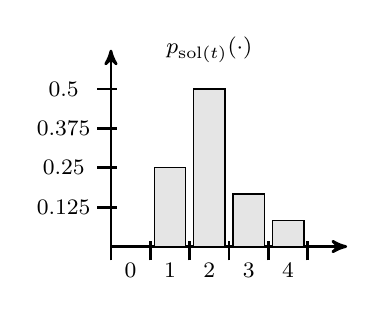
\begin{tikzpicture}[
  font=\footnotesize,
  >=stealth',
  line width=1pt,
]

\draw [<->] (0,2.5) -- (0,0) -- (3,0);
\foreach \x in {0,...,5} {
  \draw (0.5*\x,-0.175) -- (0.5*\x,0.075);
}
\foreach \x in {0,1,...,4} {
  \node (tx\x) at (0.5*\x+0.25,-0.3) {\x};
}
\foreach \x in {1,...,4} {
  \draw (-0.175,0.5*\x) -- (0.075,0.5*\x);
}
\node (tyy1) at (1.25,2.5) {$p_{\mathrm{sol}(t)}(\cdot)$};
\node (ty1) at (-0.6,0.5) {0.125};
\node (ty2) at (-0.6,1) {0.25};
\node (ty3) at (-0.6,1.5) {0.375};
\node (ty4) at (-0.6,2) {0.5};
\draw[fill=gray!20,line width=0.5pt] (0.55,0) rectangle (0.95,4/4);
\draw[fill=gray!20,line width=0.5pt] (1.05,0) rectangle (1.45,4/2);
\draw[fill=gray!20,line width=0.5pt] (1.55,0) rectangle (1.95,4/6);
\draw[fill=gray!20,line width=0.5pt] (2.05,0) rectangle (2.45,4/12);

\end{tikzpicture}
}
  \end{center}
\end{columns}
\begin{block}{Checking Condition~1: $p_{\mathrm{sol}(t)} \preceq p_{\mathrm{sol}(t+1)}$}
\begin{itemize}
\item CDF comparison yields
\begin{equation*}
\sum_{\ell=0}^m p_t(\ell) - \sum_{\ell=0}^m p_{t+1}(\ell)
= \frac{1}{t} - \frac{1}{t+1}
= \frac{1}{t(t+1)}
\end{equation*}
\item Difference vanishes for $m \geq t+1$
\item Hence $p_{\mathrm{sol}(t)} \preceq p_{\mathrm{sol}(t+1)}$
\end{itemize}
\end{block}
\end{frame}


\begin{frame}
\frametitle{Example: Soliton Distributions}
\begin{block}{Checking Condition~2: $p_{\mathrm{sol}(t+1)} \preceq S p_{\mathrm{sol}(t)}$}
\begin{itemize}
\item For $m=1$, we have
\begin{equation*}
\sum_{\ell=0}^m p_{t+1}(\ell)
- \sum_{\ell=0}^{m-1} p_t(\ell)
= \frac{1}{t+1} \geq 0
\end{equation*}
\item For $m = 2, \ldots, t$, we get
\begin{equation*}
\begin{split}
\sum_{\ell=0}^m p_{t+1}(\ell)
- \sum_{\ell=0}^{m-1} p_t(\ell)
&= \frac{1}{(m-1)m} - \frac{1}{t(t+1)} \geq 0
\end{split}
\end{equation*}
\item Difference vanishes for $m \geq t+1$
\item Hence $p_{\mathrm{sol}(t+1)} \preceq S p_{\mathrm{sol}(t)}$
\end{itemize}
\end{block}
\end{frame}


\begin{frame}
\frametitle{Example: Soliton Distributions}
\begin{itemize}
\item Conditions~1~\&~2 are \textbf{fulfilled}
\item There exits \textbf{Markov chain} containing solely self-transitions and transitions to nearest neighbors on the right that possesses \textbf{Soliton distribution} at every time~$t$
\end{itemize}
\vfill
\begin{columns}
\column{.6\textwidth}
  \begin{itemize}
  \item Transition probabilities are
  \begin{equation*}
  \gamma^{(t)}_m = \begin{cases}
  \frac{1}{t+1} & m = 1 \\
  \frac{(m-1)m}{t(t+1)} & m = 2, \ldots, t \\
  0 & \text{otherwise}
  \end{cases}
  \end{equation*}
  \item Probability that device transmit during slot~$t$ is Wasserstein distance
  \end{itemize}
\column{.35\textwidth}
  \begin{center}
  \scalebox{0.9}{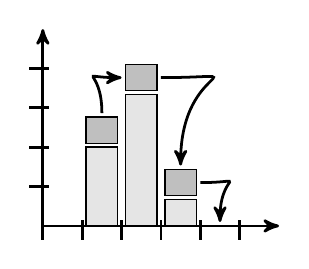
\begin{tikzpicture}[
  font=\footnotesize,
  >=stealth',
  line width=1pt,
]

\draw [<->] (0,2.5) -- (0,0) -- (3,0);
\foreach \x in {0,...,5} {
  \draw (0.5*\x,-0.175) -- (0.5*\x,0.075);
}
\foreach \x in {1,...,4} {
  \draw (-0.175,0.5*\x) -- (0.075,0.5*\x);
}
\draw[fill=gray!20,line width=0.5pt] (0.55,0) rectangle (0.95,1);
\draw[fill=gray!50,line width=0.5pt] (0.55,1+0.05) rectangle (0.95,4/3+0.05);
\draw[fill=gray!20,line width=0.5pt] (1.05,0) rectangle (1.45,5/3);
\draw[fill=gray!50,line width=0.5pt] (1.05,5/3+0.05) rectangle (1.45,2+0.05);
\draw[fill=gray!20,line width=0.5pt] (1.55,0) rectangle (1.95,1/3);
\draw[fill=gray!50,line width=0.5pt] (1.55,1/3+0.05) rectangle (1.95,2/3+0.05);

\draw [->] (0.75,4/3+0.1) to [out=90, in=180, looseness=3] (1.,11/6+0.05);
\draw [->] (1.5,11/6+0.05) to [out=0, in=90, looseness=3] (1.75,2/3+0.1);
\draw [->] (2,1/2+0.05) to [out=0, in=90, looseness=3] (2.25,0.05);

\end{tikzpicture}
}
  \end{center}
\end{columns}
\vfill
\begin{center}
\textbf{Is this complete story?}
\end{center}
\end{frame}


\begin{frame}
\frametitle{Realization of Standard Soliton Access Pattern (Goal)}
\begin{center}
  \scalebox{0.6}{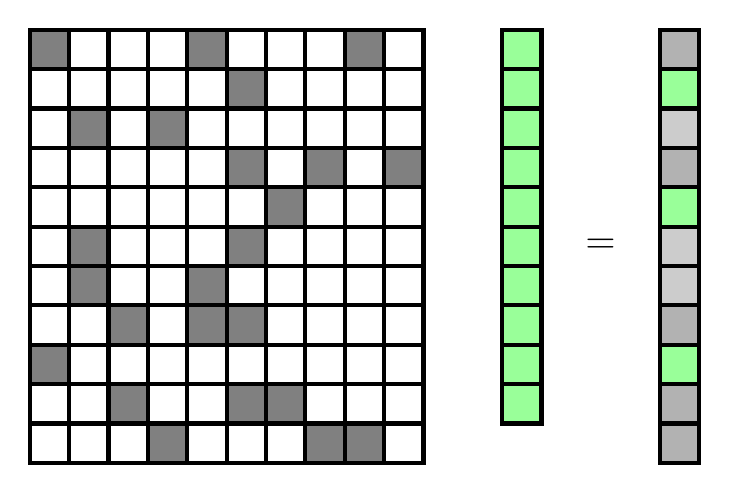
\begin{tikzpicture}
[draw=black, line width=1.5pt, >=stealth',
entry1/.style={rectangle, draw, fill=gray, inner sep=0pt, minimum size=5mm},
entry0/.style={rectangle, draw, inner sep=0pt, minimum size=5mm},
symbol/.style={rectangle, draw, fill=green!40, inner sep=0pt, minimum size=5mm}]

\node[entry0] (m00) at (0,0) {};
\node[entry0] (m01) at (0.5,0) {};
\node[entry0] (m02) at (1,0) {};
\node[entry1] (m03) at (1.5,0) {};
\node[entry0] (m04) at (2,0) {};
\node[entry0] (m05) at (2.5,0) {};
\node[entry0] (m06) at (3,0) {};
\node[entry1] (m07) at (3.5,0) {};
\node[entry1] (m08) at (4,0) {};
\node[entry0] (m09) at (4.5,0) {};

\node[entry0] (m00) at (0,0.5) {};
\node[entry0] (m11) at (0.5,0.5) {};
\node[entry1] (m12) at (1,0.5) {};
\node[entry0] (m13) at (1.5,0.5) {};
\node[entry0] (m14) at (2,0.5) {};
\node[entry1] (m15) at (2.5,0.5) {};
\node[entry1] (m16) at (3,0.5) {};
\node[entry0] (m17) at (3.5,0.5) {};
\node[entry0] (m18) at (4,0.5) {};
\node[entry0] (m19) at (4.5,0.5) {};

\node[entry1] (m20) at (0,1) {};
\node[entry0] (m21) at (0.5,1) {};
\node[entry0] (m22) at (1,1) {};
\node[entry0] (m23) at (1.5,1) {};
\node[entry0] (m24) at (2,1) {};
\node[entry0] (m25) at (2.5,1) {};
\node[entry0] (m26) at (3,1) {};
\node[entry0] (m27) at (3.5,1) {};
\node[entry0] (m28) at (4,1) {};
\node[entry0] (m29) at (4.5,1) {};

\node[entry0] (m30) at (0,1.5) {};
\node[entry0] (m31) at (0.5,1.5) {};
\node[entry1] (m32) at (1,1.5) {};
\node[entry0] (m33) at (1.5,1.5) {};
\node[entry1] (m34) at (2,1.5) {};
\node[entry1] (m35) at (2.5,1.5) {};
\node[entry0] (m36) at (3,1.5) {};
\node[entry0] (m37) at (3.5,1.5) {};
\node[entry0] (m38) at (4,1.5) {};
\node[entry0] (m39) at (4.5,1.5) {};

\node[entry0] (m40) at (0,2) {};
\node[entry1] (m41) at (0.5,2) {};
\node[entry0] (m42) at (1,2) {};
\node[entry0] (m43) at (1.5,2) {};
\node[entry1] (m44) at (2,2) {};
\node[entry0] (m45) at (2.5,2) {};
\node[entry0] (m46) at (3,2) {};
\node[entry0] (m47) at (3.5,2) {};
\node[entry0] (m48) at (4,2) {};
\node[entry0] (m49) at (4.5,2) {};

\node[entry0] (m50) at (0,2.5) {};
\node[entry1] (m51) at (0.5,2.5) {};
\node[entry0] (m52) at (1,2.5) {};
\node[entry0] (m53) at (1.5,2.5) {};
\node[entry0] (m54) at (2,2.5) {};
\node[entry1] (m55) at (2.5,2.5) {};
\node[entry0] (m56) at (3,2.5) {};
\node[entry0] (m57) at (3.5,2.5) {};
\node[entry0] (m58) at (4,2.5) {};
\node[entry0] (m59) at (4.5,2.5) {};

\node[entry0] (m60) at (0,3) {};
\node[entry0] (m61) at (0.5,3) {};
\node[entry0] (m62) at (1,3) {};
\node[entry0] (m63) at (1.5,3) {};
\node[entry0] (m64) at (2,3) {};
\node[entry0] (m65) at (2.5,3) {};
\node[entry1] (m66) at (3,3) {};
\node[entry0] (m67) at (3.5,3) {};
\node[entry0] (m68) at (4,3) {};
\node[entry0] (m69) at (4.5,3) {};

\node[entry0] (m70) at (0,3.5) {};
\node[entry0] (m71) at (0.5,3.5) {};
\node[entry0] (m72) at (1,3.5) {};
\node[entry0] (m73) at (1.5,3.5) {};
\node[entry0] (m74) at (2,3.5) {};
\node[entry1] (m75) at (2.5,3.5) {};
\node[entry0] (m76) at (3,3.5) {};
\node[entry1] (m77) at (3.5,3.5) {};
\node[entry0] (m78) at (4,3.5) {};
\node[entry1] (m79) at (4.5,3.5) {};

\node[entry0] (m80) at (0,4) {};
\node[entry1] (m81) at (0.5,4) {};
\node[entry0] (m82) at (1,4) {};
\node[entry1] (m83) at (1.5,4) {};
\node[entry0] (m84) at (2,4) {};
\node[entry0] (m85) at (2.5,4) {};
\node[entry0] (m86) at (3,4) {};
\node[entry0] (m87) at (3.5,4) {};
\node[entry0] (m88) at (4,4) {};
\node[entry0] (m89) at (4.5,4) {};

\node[entry0] (m90) at (0,4.5) {};
\node[entry0] (m91) at (0.5,4.5) {};
\node[entry0] (m92) at (1,4.5) {};
\node[entry0] (m93) at (1.5,4.5) {};
\node[entry0] (m94) at (2,4.5) {};
\node[entry1] (m95) at (2.5,4.5) {};
\node[entry0] (m96) at (3,4.5) {};
\node[entry0] (m97) at (3.5,4.5) {};
\node[entry0] (m98) at (4,4.5) {};
\node[entry0] (m99) at (4.5,4.5) {};

\node[entry1] (m100) at (0,5) {};
\node[entry0] (m101) at (0.5,5) {};
\node[entry0] (m102) at (1,5) {};
\node[entry0] (m103) at (1.5,5) {};
\node[entry1] (m104) at (2,5) {};
\node[entry0] (m105) at (2.5,5) {};
\node[entry0] (m106) at (3,5) {};
\node[entry0] (m107) at (3.5,5) {};
\node[entry1] (m108) at (4,5) {};
\node[entry0] (m109) at (4.5,5) {};


\node[symbol] (s1) at (6,0.5) {};
\node[symbol] (s2) at (6,1) {};
\node[symbol] (s3) at (6,1.5) {};
\node[symbol] (s4) at (6,2) {};
\node[symbol] (s5) at (6,2.5) {};
\node[symbol] (s6) at (6,3) {};
\node[symbol] (s7) at (6,3.5) {};
\node[symbol] (s8) at (6,4) {};
\node[symbol] (s9) at (6,4.5) {};
\node[symbol] (s10) at (6,5) {};

\node (equal) at (7,2.5) {\Large =};

\node[entry0,fill=black!30] (y0) at (8,0) {};
\node[entry0,fill=black!30] (y1) at (8,0.5) {};
\node[symbol] (y2) at (8,1) {};
\node[entry0,fill=black!30] (y3) at (8,1.5) {};
\node[entry0,fill=black!20] (y4) at (8,2) {};
\node[entry0,fill=black!20] (y5) at (8,2.5) {};
\node[symbol] (y6) at (8,3) {};
\node[entry0,fill=black!30] (y7) at (8,3.5) {};
\node[entry0,fill=black!20] (y8) at (8,4) {};
\node[entry0,symbol] (y9) at (8,4.5) {};
\node[entry0,fill=black!30] (y10) at (8,5) {};

\end{tikzpicture}

}
\end{center}
\vfill
\begin{center}
  \scalebox{0.8}{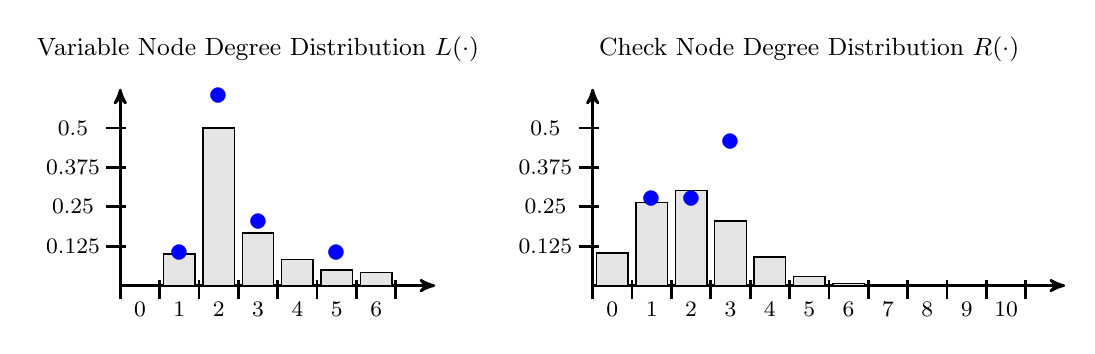
\begin{tikzpicture}[
  font=\footnotesize,
  >=stealth',
  line width=1pt,
]

\draw [<->] (0,2.5) -- (0,0) -- (4,0);
\foreach \x in {0,...,7} {
  \draw (0.5*\x,-0.175) -- (0.5*\x,0.075);
}
\foreach \x in {0,1,...,6} {
  \node (tx\x) at (0.5*\x+0.25,-0.3) {\x};
}
\foreach \x in {1,...,4} {
  \draw (-0.175,0.5*\x) -- (0.075,0.5*\x);
}
\node (tyy1) at (1.75,3) {\small Variable Node Degree Distribution $L(\cdot)$};
\node (ty1) at (-0.6,0.5) {0.125};
\node (ty2) at (-0.6,1) {0.25};
\node (ty3) at (-0.6,1.5) {0.375};
\node (ty4) at (-0.6,2) {0.5};
\draw[fill=gray!20,line width=0.5pt] (0.55,0) rectangle (0.95,4/10);
\draw[fill=gray!20,line width=0.5pt] (1.05,0) rectangle (1.45,4/2);
\draw[fill=gray!20,line width=0.5pt] (1.55,0) rectangle (1.95,4/6);
\draw[fill=gray!20,line width=0.5pt] (2.05,0) rectangle (2.45,4/12);
\draw[fill=gray!20,line width=0.5pt] (2.55,0) rectangle (2.95,4/20);
\draw[fill=gray!20,line width=0.5pt] (3.05,0) rectangle (3.45,4/24);

\node at (0.75,4/10) {\Large \textcolor{blue}{$\bullet$}};
\node at (1.25,24/10) {\Large \textcolor{blue}{$\bullet$}};
\node at (1.75,8/10) {\Large \textcolor{blue}{$\bullet$}};
\node at (2.75,4/10) {\Large \textcolor{blue}{$\bullet$}};

\draw [<->] (6,2.5) -- (6,0) -- (12,0);
\foreach \x in {0,...,11} {
  \draw (0.5*\x+6,-0.175) -- (0.5*\x+6,0.075);
}
\foreach \x in {0,1,...,10} {
  \node (txx\x) at (0.5*\x+6.25,-0.3) {\x};
}
\foreach \x in {1,...,4} {
  \draw (6-0.175,0.5*\x) -- (6.075,0.5*\x);
}
\node (tyy1) at (8.75,3) {\small Check Node Degree Distribution $R(\cdot)$};
\node (tyy1) at (6-0.6,0.5) {0.125};
\node (tyy2) at (6-0.6,1) {0.25};
\node (tyy3) at (6-0.6,1.5) {0.375};
\node (tyy4) at (6-0.6,2) {0.5};
\draw[fill=gray!20,line width=0.5pt] (6.05,0) rectangle (6.45,0.414);
\draw[fill=gray!20,line width=0.5pt] (6.55,0) rectangle (6.95,1.054);
\draw[fill=gray!20,line width=0.5pt] (7.05,0) rectangle (7.45,1.208);
\draw[fill=gray!20,line width=0.5pt] (7.55,0) rectangle (7.95,0.820);
\draw[fill=gray!20,line width=0.5pt] (8.05,0) rectangle (8.45,0.365);
\draw[fill=gray!20,line width=0.5pt] (8.55,0) rectangle (8.95,0.112);
\draw[fill=gray!20,line width=0.5pt] (9.05,0) rectangle (9.45,0.024);
\draw[fill=gray!20,line width=0.5pt] (9.55,0) rectangle (9.95,0.003);

\node at (6.75,12/11) {\Large \textcolor{blue}{$\bullet$}};
\node at (7.25,12/11) {\Large \textcolor{blue}{$\bullet$}};
\node at (7.75,20/11) {\Large \textcolor{blue}{$\bullet$}};

\end{tikzpicture}
}
\end{center}
\end{frame}


\begin{frame}
\frametitle{Realization of Markov Soliton Access Pattern (Outcome)}
\begin{center}
  \scalebox{0.6}{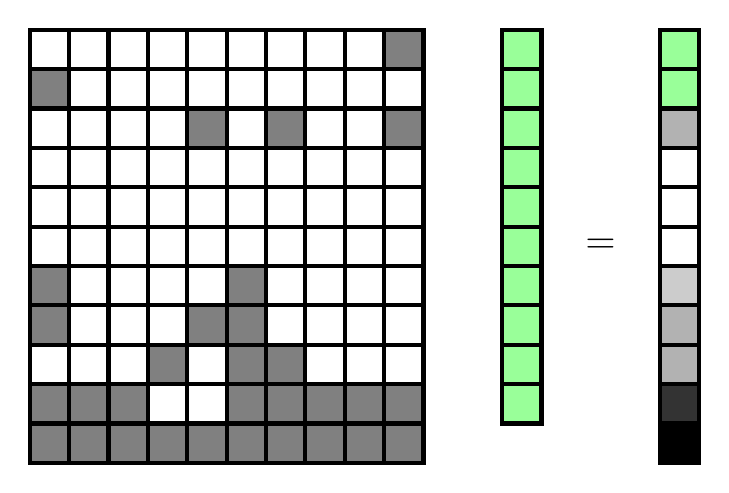
\begin{tikzpicture}
[draw=black, line width=1.5pt, >=stealth',
entry1/.style={rectangle, draw, fill=gray, inner sep=0pt, minimum size=5mm},
entry0/.style={rectangle, draw, inner sep=0pt, minimum size=5mm},
symbol/.style={rectangle, draw, fill=green!40, inner sep=0pt, minimum size=5mm}]

\node[entry1] (m00) at (0,0) {};
\node[entry1] (m01) at (0.5,0) {};
\node[entry1] (m02) at (1,0) {};
\node[entry1] (m03) at (1.5,0) {};
\node[entry1] (m04) at (2,0) {};
\node[entry1] (m05) at (2.5,0) {};
\node[entry1] (m06) at (3,0) {};
\node[entry1] (m07) at (3.5,0) {};
\node[entry1] (m08) at (4,0) {};
\node[entry1] (m09) at (4.5,0) {};

\node[entry1] (m00) at (0,0.5) {};
\node[entry1] (m11) at (0.5,0.5) {};
\node[entry1] (m12) at (1,0.5) {};
\node[entry0] (m13) at (1.5,0.5) {};
\node[entry0] (m14) at (2,0.5) {};
\node[entry1] (m15) at (2.5,0.5) {};
\node[entry1] (m16) at (3,0.5) {};
\node[entry1] (m17) at (3.5,0.5) {};
\node[entry1] (m18) at (4,0.5) {};
\node[entry1] (m19) at (4.5,0.5) {};

\node[entry0] (m20) at (0,1) {};
\node[entry0] (m21) at (0.5,1) {};
\node[entry0] (m22) at (1,1) {};
\node[entry1] (m23) at (1.5,1) {};
\node[entry0] (m24) at (2,1) {};
\node[entry1] (m25) at (2.5,1) {};
\node[entry1] (m26) at (3,1) {};
\node[entry0] (m27) at (3.5,1) {};
\node[entry0] (m28) at (4,1) {};
\node[entry0] (m29) at (4.5,1) {};

\node[entry1] (m30) at (0,1.5) {};
\node[entry0] (m31) at (0.5,1.5) {};
\node[entry0] (m32) at (1,1.5) {};
\node[entry0] (m33) at (1.5,1.5) {};
\node[entry1] (m34) at (2,1.5) {};
\node[entry1] (m35) at (2.5,1.5) {};
\node[entry0] (m36) at (3,1.5) {};
\node[entry0] (m37) at (3.5,1.5) {};
\node[entry0] (m38) at (4,1.5) {};
\node[entry0] (m39) at (4.5,1.5) {};

\node[entry1] (m40) at (0,2) {};
\node[entry0] (m41) at (0.5,2) {};
\node[entry0] (m42) at (1,2) {};
\node[entry0] (m43) at (1.5,2) {};
\node[entry0] (m44) at (2,2) {};
\node[entry1] (m45) at (2.5,2) {};
\node[entry0] (m46) at (3,2) {};
\node[entry0] (m47) at (3.5,2) {};
\node[entry0] (m48) at (4,2) {};
\node[entry0] (m49) at (4.5,2) {};

\node[entry0] (m50) at (0,2.5) {};
\node[entry0] (m51) at (0.5,2.5) {};
\node[entry0] (m52) at (1,2.5) {};
\node[entry0] (m53) at (1.5,2.5) {};
\node[entry0] (m54) at (2,2.5) {};
\node[entry0] (m55) at (2.5,2.5) {};
\node[entry0] (m56) at (3,2.5) {};
\node[entry0] (m57) at (3.5,2.5) {};
\node[entry0] (m58) at (4,2.5) {};
\node[entry0] (m59) at (4.5,2.5) {};

\node[entry0] (m60) at (0,3) {};
\node[entry0] (m61) at (0.5,3) {};
\node[entry0] (m62) at (1,3) {};
\node[entry0] (m63) at (1.5,3) {};
\node[entry0] (m64) at (2,3) {};
\node[entry0] (m65) at (2.5,3) {};
\node[entry0] (m66) at (3,3) {};
\node[entry0] (m67) at (3.5,3) {};
\node[entry0] (m68) at (4,3) {};
\node[entry0] (m69) at (4.5,3) {};

\node[entry0] (m70) at (0,3.5) {};
\node[entry0] (m71) at (0.5,3.5) {};
\node[entry0] (m72) at (1,3.5) {};
\node[entry0] (m73) at (1.5,3.5) {};
\node[entry0] (m74) at (2,3.5) {};
\node[entry0] (m75) at (2.5,3.5) {};
\node[entry0] (m76) at (3,3.5) {};
\node[entry0] (m77) at (3.5,3.5) {};
\node[entry0] (m78) at (4,3.5) {};
\node[entry0] (m79) at (4.5,3.5) {};

\node[entry0] (m80) at (0,4) {};
\node[entry0] (m81) at (0.5,4) {};
\node[entry0] (m82) at (1,4) {};
\node[entry0] (m83) at (1.5,4) {};
\node[entry1] (m84) at (2,4) {};
\node[entry0] (m85) at (2.5,4) {};
\node[entry1] (m86) at (3,4) {};
\node[entry0] (m87) at (3.5,4) {};
\node[entry0] (m88) at (4,4) {};
\node[entry1] (m89) at (4.5,4) {};

\node[entry1] (m90) at (0,4.5) {};
\node[entry0] (m91) at (0.5,4.5) {};
\node[entry0] (m92) at (1,4.5) {};
\node[entry0] (m93) at (1.5,4.5) {};
\node[entry0] (m94) at (2,4.5) {};
\node[entry0] (m95) at (2.5,4.5) {};
\node[entry0] (m96) at (3,4.5) {};
\node[entry0] (m97) at (3.5,4.5) {};
\node[entry0] (m98) at (4,4.5) {};
\node[entry0] (m99) at (4.5,4.5) {};

\node[entry0] (m100) at (0,5) {};
\node[entry0] (m101) at (0.5,5) {};
\node[entry0] (m102) at (1,5) {};
\node[entry0] (m103) at (1.5,5) {};
\node[entry0] (m104) at (2,5) {};
\node[entry0] (m105) at (2.5,5) {};
\node[entry0] (m106) at (3,5) {};
\node[entry0] (m107) at (3.5,5) {};
\node[entry0] (m108) at (4,5) {};
\node[entry1] (m109) at (4.5,5) {};


\node[symbol] (s1) at (6,0.5) {};
\node[symbol] (s2) at (6,1) {};
\node[symbol] (s3) at (6,1.5) {};
\node[symbol] (s4) at (6,2) {};
\node[symbol] (s5) at (6,2.5) {};
\node[symbol] (s6) at (6,3) {};
\node[symbol] (s7) at (6,3.5) {};
\node[symbol] (s8) at (6,4) {};
\node[symbol] (s9) at (6,4.5) {};
\node[symbol] (s10) at (6,5) {};

\node (equal) at (7,2.5) {\Large =};

\node[entry0,fill=black!100] (y0) at (8,0) {};
\node[entry0,fill=black!80] (y1) at (8,0.5) {};
\node[entry0,fill=black!30] (y2) at (8,1) {};
\node[entry0,fill=black!30] (y3) at (8,1.5) {};
\node[entry0,fill=black!20] (y4) at (8,2) {};
\node[entry0,fill=white] (y5) at (8,2.5) {};
\node[entry0,fill=white] (y6) at (8,3) {};
\node[entry0,fill=white] (y7) at (8,3.5) {};
\node[entry0,fill=black!30] (y8) at (8,4) {};
\node[symbol] (y9) at (8,4.5) {};
\node[symbol] (y10) at (8,5) {};

\end{tikzpicture}

}
\end{center}
\vfill
\begin{center}
  \scalebox{0.8}{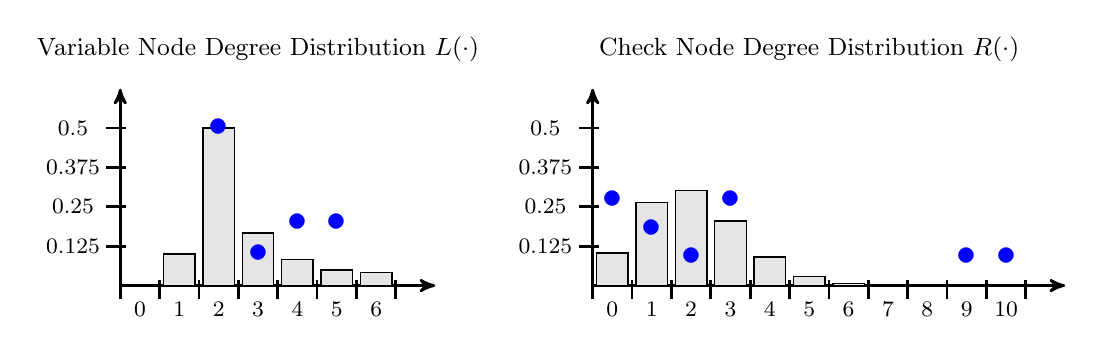
\begin{tikzpicture}[
  font=\footnotesize,
  >=stealth',
  line width=1pt,
]

\draw [<->] (0,2.5) -- (0,0) -- (4,0);
\foreach \x in {0,...,7} {
  \draw (0.5*\x,-0.175) -- (0.5*\x,0.075);
}
\foreach \x in {0,1,...,6} {
  \node (tx\x) at (0.5*\x+0.25,-0.3) {\x};
}
\foreach \x in {1,...,4} {
  \draw (-0.175,0.5*\x) -- (0.075,0.5*\x);
}
\node (tyy1) at (1.75,3) {\small Variable Node Degree Distribution $L(\cdot)$};
\node (ty1) at (-0.6,0.5) {0.125};
\node (ty2) at (-0.6,1) {0.25};
\node (ty3) at (-0.6,1.5) {0.375};
\node (ty4) at (-0.6,2) {0.5};
\draw[fill=gray!20,line width=0.5pt] (0.55,0) rectangle (0.95,4/10);
\draw[fill=gray!20,line width=0.5pt] (1.05,0) rectangle (1.45,4/2);
\draw[fill=gray!20,line width=0.5pt] (1.55,0) rectangle (1.95,4/6);
\draw[fill=gray!20,line width=0.5pt] (2.05,0) rectangle (2.45,4/12);
\draw[fill=gray!20,line width=0.5pt] (2.55,0) rectangle (2.95,4/20);
\draw[fill=gray!20,line width=0.5pt] (3.05,0) rectangle (3.45,4/24);

\node at (1.25,20/10) {\Large \textcolor{blue}{$\bullet$}};
\node at (1.75,4/10) {\Large \textcolor{blue}{$\bullet$}};
\node at (2.25,8/10) {\Large \textcolor{blue}{$\bullet$}};
\node at (2.75,8/10) {\Large \textcolor{blue}{$\bullet$}};

\draw [<->] (6,2.5) -- (6,0) -- (12,0);
\foreach \x in {0,...,11} {
  \draw (0.5*\x+6,-0.175) -- (0.5*\x+6,0.075);
}
\foreach \x in {0,1,...,10} {
  \node (txx\x) at (0.5*\x+6.25,-0.3) {\x};
}
\foreach \x in {1,...,4} {
  \draw (6-0.175,0.5*\x) -- (6.075,0.5*\x);
}
\node (tyy1) at (8.75,3) {\small Check Node Degree Distribution $R(\cdot)$};
\node (tyy1) at (6-0.6,0.5) {0.125};
\node (tyy2) at (6-0.6,1) {0.25};
\node (tyy3) at (6-0.6,1.5) {0.375};
\node (tyy4) at (6-0.6,2) {0.5};
\draw[fill=gray!20,line width=0.5pt] (6.05,0) rectangle (6.45,0.414);
\draw[fill=gray!20,line width=0.5pt] (6.55,0) rectangle (6.95,1.054);
\draw[fill=gray!20,line width=0.5pt] (7.05,0) rectangle (7.45,1.208);
\draw[fill=gray!20,line width=0.5pt] (7.55,0) rectangle (7.95,0.820);
\draw[fill=gray!20,line width=0.5pt] (8.05,0) rectangle (8.45,0.365);
\draw[fill=gray!20,line width=0.5pt] (8.55,0) rectangle (8.95,0.112);
\draw[fill=gray!20,line width=0.5pt] (9.05,0) rectangle (9.45,0.024);
\draw[fill=gray!20,line width=0.5pt] (9.55,0) rectangle (9.95,0.003);

\node at (6.25,12/11) {\Large \textcolor{blue}{$\bullet$}};
\node at (6.75,8/11) {\Large \textcolor{blue}{$\bullet$}};
\node at (7.25,4/11) {\Large \textcolor{blue}{$\bullet$}};
\node at (7.75,12/11) {\Large \textcolor{blue}{$\bullet$}};
\node at (10.75,4/11) {\Large \textcolor{blue}{$\bullet$}};
\node at (11.25,4/11) {\Large \textcolor{blue}{$\bullet$}};

\end{tikzpicture}
}
\end{center}
\end{frame}


\begin{frame}
\frametitle{Universal Framework with Markov Transmission Scheme}
\begin{itemize}
\item Access point solely broadcast start/end of round
\item Devices employ Markov chain to elect when to transmit
\item Mathematical framework provide methodology to shape marginal distributions at every time step
\end{itemize}
\begin{block}{Positive Aspects}
\begin{itemize}
\item Design space is large in terms of distribution shaping
\item Slot count can differ from number of active devices
\item Stopping condition can include state of peeling decoder
\end{itemize}
\end{block}
\begin{block}{Limitations}
\begin{itemize}
\item Probability that device transmit packet is not uniform over time
\item Tanner graph may be front-loaded
\item Uniformly optimal universal scheme may not exist 
\end{itemize}
\end{block}
\end{frame}


\begin{frame}
\frametitle{Candidate Distributions Used in Numerical Results}
\begin{block}{Stateless Distributions}
\begin{itemize}
\item Device use emission probabilities based on time elapsed
\end{itemize}
\begin{equation*}
\gamma^{(t)}_m = \gamma^{(t)}
= 1 - \exp \left( \frac{c \log(\epsilon)}{t} \right)
\end{equation*}
\end{block}
\begin{block}{Skewed Distributions}
\begin{itemize}
\item Skewed family favors nodes that have transmitted several packets
\end{itemize}
\begin{equation*}
\gamma_m^{(t)} = \begin{cases}
0, & \sum_{i=0}^m p_t(i) < 1 - \overline{\gamma}^{(t)} \\
1, & \sum_{i=m}^{t} p_t(i) \leq \overline{\gamma}^{(t)} \\
\frac{\overline{\gamma}^{(t)} - \sum_{i=m+1}^{t} p_t(i)}{p_t(m)}
& \text{otherwise}
\end{cases}
\end{equation*}
\end{block}
\begin{block}{Skewed Distributions}
\begin{center}
In numerical results, we use mixture of these two families
\end{center}
\end{block}
\end{frame}



\begin{frame}
\frametitle{Numerical Results -- Parameterized Distribution}
\begin{itemize}
\item Parameter~1: Number of time slots per round
\item Parameter~2: Tuning factor to favor nodes that have already transmitted several copies of their messages
\item \textbf{Performance Criterion:} average number of decoded packet per time slot (shown for 1250~devices)
\end{itemize}
\begin{center}
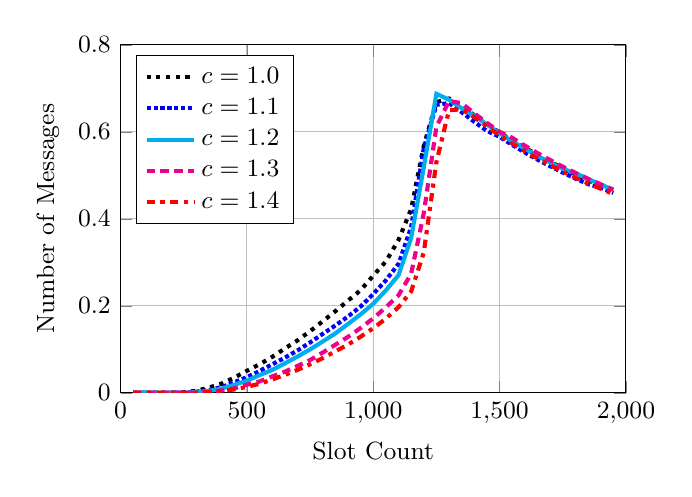
\begin{tikzpicture}
\begin{axis}[
  width=8cm,
  height=6cm,
  font=\small,
  xlabel={Slot Count},
  ylabel={Number of Messages},
  xmajorgrids,
  ymajorgrids,
  ymin=0,
  ymax=0.8,
  xmin=0,
  xmax=2000,
  legend entries={$c=1.0$,$c=1.1$,$c=1.2$,$c=1.3$,$c=1.4$},
  legend style={legend pos=north west,nodes=right}]
\addplot [
color=black,
line width=1.5pt,
dotted
]
coordinates{ (50,0.0) (100,0.0)
(150,6.66666666667e-05) (200,0.00045)
(250,0.00132) (300,0.00466666666667)
(350,0.0119714285714) (400,0.0212)
(450,0.0348888888889) (500,0.0506)
(550,0.0654181818182) (600,0.0825)
(650,0.101707692308) (700,0.120428571429)
(750,0.141613333333) (800,0.1643875)
(850,0.187541176471) (900,0.211922222222)
(950,0.235894736842) (1000,0.26947)
(1050,0.301904761905) (1100,0.351327272727)
(1150,0.422147826087) (1200,0.567533333333)
(1250,0.668288) (1300,0.676623076923)
(1350,0.658088888889) (1400,0.638178571429)
(1450,0.618020689655) (1500,0.598426666667)
(1550,0.580135483871) (1600,0.5635625)
(1650,0.546921212121) (1700,0.531323529412)
(1750,0.516708571429) (1800,0.502644444444)
(1850,0.489486486486) (1900,0.476868421053)
(1950,0.464892307692) };
\addplot [
color=blue,
line width=1.5pt,
densely dotted
]
coordinates{ (50,0.0) (100,0.0)
(150,0.0) (200,0.00015)
(250,0.0008) (300,0.00266666666667)
(350,0.00637142857143) (400,0.013225)
(450,0.0240222222222) (500,0.03594)
(550,0.0501636363636) (600,0.0652666666667)
(650,0.0806153846154) (700,0.0972142857143)
(750,0.11564) (800,0.135425)
(850,0.154694117647) (900,0.175366666667)
(950,0.198357894737) (1000,0.22715)
(1050,0.258628571429) (1100,0.296381818182)
(1150,0.380591304348) (1200,0.562483333333)
(1250,0.662248) (1300,0.666284615385)
(1350,0.645259259259) (1400,0.623171428571)
(1450,0.602248275862) (1500,0.5886)
(1550,0.570135483871) (1600,0.5526625)
(1650,0.536345454545) (1700,0.521035294118)
(1750,0.506594285714) (1800,0.492761111111)
(1850,0.479881081081) (1900,0.471668421053)
(1950,0.459887179487) };
\addplot [
color=cyan,
line width=1.5pt,
solid
]
coordinates{ (50,0.0) (100,0.0)
(150,0.0) (200,0.0)
(250,0.00024) (300,0.0015)
(350,0.00428571428571) (400,0.0098)
(450,0.0183777777778) (500,0.02786)
(550,0.0406363636364) (600,0.0524666666667)
(650,0.0676) (700,0.0831857142857)
(750,0.0996666666667) (800,0.1178375)
(850,0.136552941176) (900,0.158111111111)
(950,0.180305263158) (1000,0.20481)
(1050,0.235466666667) (1100,0.270345454545)
(1150,0.355895652174) (1200,0.518383333333)
(1250,0.687336) (1300,0.674215384615)
(1350,0.654074074074) (1400,0.637285714286)
(1450,0.616931034483) (1500,0.596966666667)
(1550,0.578225806452) (1600,0.5616125)
(1650,0.544890909091) (1700,0.529711764706)
(1750,0.514851428571) (1800,0.505288888889)
(1850,0.491697297297) (1900,0.479010526316)
(1950,0.466912820513) };
\addplot [
color=magenta,
line width=1.5pt,
densely dashed
]
coordinates{ (50,0.0) (100,0.0)
(150,0.0) (200,0.0)
(250,0.0) (300,0.0004)
(350,0.00185714285714) (400,0.00525)
(450,0.0102) (500,0.01866)
(550,0.0261818181818) (600,0.0376)
(650,0.0484769230769) (700,0.0617142857143)
(750,0.0752666666667) (800,0.0924125)
(850,0.110447058824) (900,0.128477777778)
(950,0.148957894737) (1000,0.17123)
(1050,0.19659047619) (1100,0.224263636364)
(1150,0.273608695652) (1200,0.412608333333)
(1250,0.611608) (1300,0.671076923077)
(1350,0.665977777778) (1400,0.642592857143)
(1450,0.62075862069) (1500,0.60026)
(1550,0.586490322581) (1600,0.56835625)
(1650,0.551321212121) (1700,0.535205882353)
(1750,0.520028571429) (1800,0.505794444444)
(1850,0.492232432432) (1900,0.479384210526)
(1950,0.467225641026) };
\addplot [
color=red,
line width=1.5pt,
dashdotted
]
coordinates{ (50,0.0) (100,0.0)
(150,0.0) (200,0.0)
(250,8e-05) (300,0.000433333333333)
(350,0.00157142857143) (400,0.00395)
(450,0.0078) (500,0.0137)
(550,0.0208) (600,0.0304333333333)
(650,0.0411692307692) (700,0.0526142857143)
(750,0.0653466666667) (800,0.07975)
(850,0.0952235294118) (900,0.110922222222)
(950,0.128873684211) (1000,0.14853)
(1050,0.170533333333) (1100,0.197027272727)
(1150,0.232852173913) (1200,0.322275)
(1250,0.53052) (1300,0.649992307692)
(1350,0.651844444444) (1400,0.6337)
(1450,0.612262068966) (1500,0.59202)
(1550,0.573187096774) (1600,0.55564375)
(1650,0.539193939394) (1700,0.523482352941)
(1750,0.508805714286) (1800,0.494822222222)
(1850,0.481632432432) (1900,0.469247368421)
(1950,0.457333333333) };
\end{axis}
\end{tikzpicture}


\end{center}
\end{frame}


\begin{frame}
\frametitle{Discussion -- Universal Framework}
\begin{itemize}
\item New framework for Universal Multiple Access
\item Necessary and sufficient conditions for proposed approach
\item Large design space need to be explored
\item Efficiency shown up to 69 percent
\item Substantially exceeds performance of traditional ALOHA
\item Performance and complexity need to be compared with case where number of devices is estimated at onset of every round
\end{itemize}
\end{frame}


\begin{frame}{Unsourced MAC}
\begin{block}{Assumptions}
\begin{itemize}
\item $K$ active devices out of $Q$ devices
\item $Q$ is very large, and $K$ is much less than $Q$
\item Every device transmits a message
\end{itemize}
\end{block}
\centerline{\textbf{Access point interested in messages, not in identity of sources}}
\begin{block}{Entropy of Identities}
\begin{itemize}
\item Size of active subset is $K$
\item Link identity of source to every message
\begin{equation*}
\log_2 \frac{Q!}{(Q-K)!}
= \mathcal{O} \left( K \log_2 Q \right)
\end{equation*}
\item Explore alternate approches
\item Performance bounds for Unsourced MAC with finite-length codes
\footnote[1]{
Y. Polyanskiy. ``A perspective on massive random access.'' ISIT, 2017.}
\end{itemize}
\end{block}
\end{frame}


\begin{frame}
\frametitle{Unsourced MAC -- Compressive Sensing Viewpoint}
\begin{center}
\scalebox{0.55}{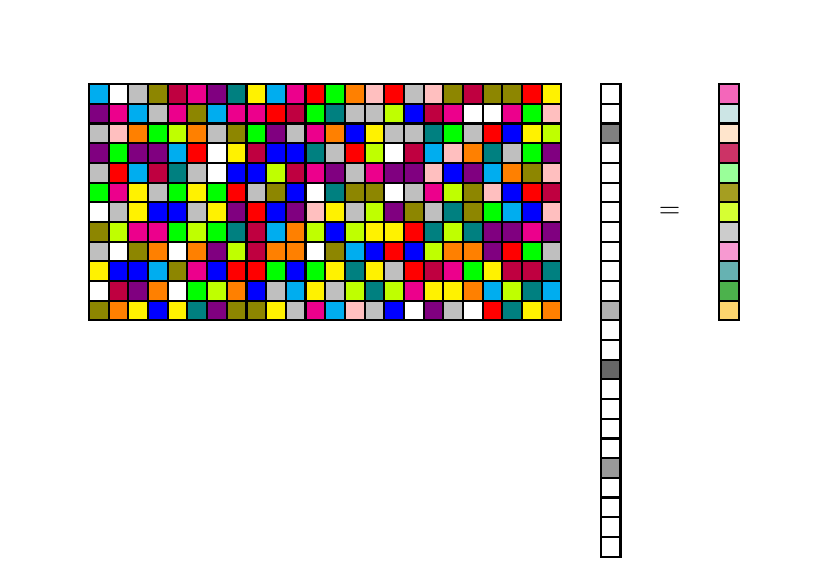
\begin{tikzpicture}
[draw=black, line width=0.75pt,
entry/.style={rectangle, draw, inner sep=0pt, minimum size=2.5mm},
symbol/.style={rectangle, draw, inner sep=0pt, minimum size=2.5mm}]

\node[entry, fill=olive] (x0y0) at (0.0,0.0) {};
\node[entry, fill=white] (x0y1) at (0.0,0.25) {};
\node[entry, fill=yellow] (x0y2) at (0.0,0.5) {};
\node[entry, fill=lightgray] (x0y3) at (0.0,0.75) {};
\node[entry, fill=olive] (x0y4) at (0.0,1.0) {};
\node[entry, fill=white] (x0y5) at (0.0,1.25) {};
\node[entry, fill=green] (x0y6) at (0.0,1.5) {};
\node[entry, fill=lightgray] (x0y7) at (0.0,1.75) {};
\node[entry, fill=violet] (x0y8) at (0.0,2.0) {};
\node[entry, fill=lightgray] (x0y9) at (0.0,2.25) {};
\node[entry, fill=violet] (x0y10) at (0.0,2.5) {};
\node[entry, fill=cyan] (x0y11) at (0.0,2.75) {};

\node[entry, fill=orange] (x1y0) at (0.25,0.0) {};
\node[entry, fill=purple] (x1y1) at (0.25,0.25) {};
\node[entry, fill=blue] (x1y2) at (0.25,0.5) {};
\node[entry, fill=white] (x1y3) at (0.25,0.75) {};
\node[entry, fill=lime] (x1y4) at (0.25,1.0) {};
\node[entry, fill=lightgray] (x1y5) at (0.25,1.25) {};
\node[entry, fill=magenta] (x1y6) at (0.25,1.5) {};
\node[entry, fill=red] (x1y7) at (0.25,1.75) {};
\node[entry, fill=green] (x1y8) at (0.25,2.0) {};
\node[entry, fill=pink] (x1y9) at (0.25,2.25) {};
\node[entry, fill=magenta] (x1y10) at (0.25,2.5) {};
\node[entry, fill=white] (x1y11) at (0.25,2.75) {};

\node[entry, fill=yellow] (x2y0) at (0.5,0.0) {};
\node[entry, fill=violet] (x2y1) at (0.5,0.25) {};
\node[entry, fill=blue] (x2y2) at (0.5,0.5) {};
\node[entry, fill=olive] (x2y3) at (0.5,0.75) {};
\node[entry, fill=magenta] (x2y4) at (0.5,1.0) {};
\node[entry, fill=yellow] (x2y5) at (0.5,1.25) {};
\node[entry, fill=yellow] (x2y6) at (0.5,1.5) {};
\node[entry, fill=cyan] (x2y7) at (0.5,1.75) {};
\node[entry, fill=violet] (x2y8) at (0.5,2.0) {};
\node[entry, fill=orange] (x2y9) at (0.5,2.25) {};
\node[entry, fill=cyan] (x2y10) at (0.5,2.5) {};
\node[entry, fill=lightgray] (x2y11) at (0.5,2.75) {};

\node[entry, fill=blue] (x3y0) at (0.75,0.0) {};
\node[entry, fill=orange] (x3y1) at (0.75,0.25) {};
\node[entry, fill=cyan] (x3y2) at (0.75,0.5) {};
\node[entry, fill=orange] (x3y3) at (0.75,0.75) {};
\node[entry, fill=magenta] (x3y4) at (0.75,1.0) {};
\node[entry, fill=blue] (x3y5) at (0.75,1.25) {};
\node[entry, fill=lightgray] (x3y6) at (0.75,1.5) {};
\node[entry, fill=purple] (x3y7) at (0.75,1.75) {};
\node[entry, fill=violet] (x3y8) at (0.75,2.0) {};
\node[entry, fill=green] (x3y9) at (0.75,2.25) {};
\node[entry, fill=lightgray] (x3y10) at (0.75,2.5) {};
\node[entry, fill=olive] (x3y11) at (0.75,2.75) {};

\node[entry, fill=yellow] (x4y0) at (1.0,0.0) {};
\node[entry, fill=white] (x4y1) at (1.0,0.25) {};
\node[entry, fill=olive] (x4y2) at (1.0,0.5) {};
\node[entry, fill=white] (x4y3) at (1.0,0.75) {};
\node[entry, fill=green] (x4y4) at (1.0,1.0) {};
\node[entry, fill=blue] (x4y5) at (1.0,1.25) {};
\node[entry, fill=green] (x4y6) at (1.0,1.5) {};
\node[entry, fill=teal] (x4y7) at (1.0,1.75) {};
\node[entry, fill=cyan] (x4y8) at (1.0,2.0) {};
\node[entry, fill=lime] (x4y9) at (1.0,2.25) {};
\node[entry, fill=magenta] (x4y10) at (1.0,2.5) {};
\node[entry, fill=purple] (x4y11) at (1.0,2.75) {};

\node[entry, fill=teal] (x5y0) at (1.25,0.0) {};
\node[entry, fill=green] (x5y1) at (1.25,0.25) {};
\node[entry, fill=magenta] (x5y2) at (1.25,0.5) {};
\node[entry, fill=orange] (x5y3) at (1.25,0.75) {};
\node[entry, fill=lime] (x5y4) at (1.25,1.0) {};
\node[entry, fill=lightgray] (x5y5) at (1.25,1.25) {};
\node[entry, fill=yellow] (x5y6) at (1.25,1.5) {};
\node[entry, fill=lightgray] (x5y7) at (1.25,1.75) {};
\node[entry, fill=red] (x5y8) at (1.25,2.0) {};
\node[entry, fill=orange] (x5y9) at (1.25,2.25) {};
\node[entry, fill=olive] (x5y10) at (1.25,2.5) {};
\node[entry, fill=magenta] (x5y11) at (1.25,2.75) {};

\node[entry, fill=violet] (x6y0) at (1.5,0.0) {};
\node[entry, fill=lime] (x6y1) at (1.5,0.25) {};
\node[entry, fill=blue] (x6y2) at (1.5,0.5) {};
\node[entry, fill=violet] (x6y3) at (1.5,0.75) {};
\node[entry, fill=green] (x6y4) at (1.5,1.0) {};
\node[entry, fill=yellow] (x6y5) at (1.5,1.25) {};
\node[entry, fill=green] (x6y6) at (1.5,1.5) {};
\node[entry, fill=white] (x6y7) at (1.5,1.75) {};
\node[entry, fill=white] (x6y8) at (1.5,2.0) {};
\node[entry, fill=lightgray] (x6y9) at (1.5,2.25) {};
\node[entry, fill=cyan] (x6y10) at (1.5,2.5) {};
\node[entry, fill=violet] (x6y11) at (1.5,2.75) {};

\node[entry, fill=olive] (x7y0) at (1.75,0.0) {};
\node[entry, fill=orange] (x7y1) at (1.75,0.25) {};
\node[entry, fill=red] (x7y2) at (1.75,0.5) {};
\node[entry, fill=lime] (x7y3) at (1.75,0.75) {};
\node[entry, fill=teal] (x7y4) at (1.75,1.0) {};
\node[entry, fill=violet] (x7y5) at (1.75,1.25) {};
\node[entry, fill=red] (x7y6) at (1.75,1.5) {};
\node[entry, fill=blue] (x7y7) at (1.75,1.75) {};
\node[entry, fill=yellow] (x7y8) at (1.75,2.0) {};
\node[entry, fill=olive] (x7y9) at (1.75,2.25) {};
\node[entry, fill=magenta] (x7y10) at (1.75,2.5) {};
\node[entry, fill=teal] (x7y11) at (1.75,2.75) {};

\node[entry, fill=olive] (x8y0) at (2.0,0.0) {};
\node[entry, fill=blue] (x8y1) at (2.0,0.25) {};
\node[entry, fill=red] (x8y2) at (2.0,0.5) {};
\node[entry, fill=purple] (x8y3) at (2.0,0.75) {};
\node[entry, fill=purple] (x8y4) at (2.0,1.0) {};
\node[entry, fill=red] (x8y5) at (2.0,1.25) {};
\node[entry, fill=lightgray] (x8y6) at (2.0,1.5) {};
\node[entry, fill=blue] (x8y7) at (2.0,1.75) {};
\node[entry, fill=purple] (x8y8) at (2.0,2.0) {};
\node[entry, fill=green] (x8y9) at (2.0,2.25) {};
\node[entry, fill=magenta] (x8y10) at (2.0,2.5) {};
\node[entry, fill=yellow] (x8y11) at (2.0,2.75) {};

\node[entry, fill=yellow] (x9y0) at (2.25,0.0) {};
\node[entry, fill=lightgray] (x9y1) at (2.25,0.25) {};
\node[entry, fill=green] (x9y2) at (2.25,0.5) {};
\node[entry, fill=orange] (x9y3) at (2.25,0.75) {};
\node[entry, fill=cyan] (x9y4) at (2.25,1.0) {};
\node[entry, fill=blue] (x9y5) at (2.25,1.25) {};
\node[entry, fill=olive] (x9y6) at (2.25,1.5) {};
\node[entry, fill=lime] (x9y7) at (2.25,1.75) {};
\node[entry, fill=blue] (x9y8) at (2.25,2.0) {};
\node[entry, fill=violet] (x9y9) at (2.25,2.25) {};
\node[entry, fill=red] (x9y10) at (2.25,2.5) {};
\node[entry, fill=cyan] (x9y11) at (2.25,2.75) {};

\node[entry, fill=lightgray] (x10y0) at (2.5,0.0) {};
\node[entry, fill=cyan] (x10y1) at (2.5,0.25) {};
\node[entry, fill=blue] (x10y2) at (2.5,0.5) {};
\node[entry, fill=orange] (x10y3) at (2.5,0.75) {};
\node[entry, fill=orange] (x10y4) at (2.5,1.0) {};
\node[entry, fill=violet] (x10y5) at (2.5,1.25) {};
\node[entry, fill=blue] (x10y6) at (2.5,1.5) {};
\node[entry, fill=purple] (x10y7) at (2.5,1.75) {};
\node[entry, fill=blue] (x10y8) at (2.5,2.0) {};
\node[entry, fill=lightgray] (x10y9) at (2.5,2.25) {};
\node[entry, fill=purple] (x10y10) at (2.5,2.5) {};
\node[entry, fill=magenta] (x10y11) at (2.5,2.75) {};

\node[entry, fill=magenta] (x11y0) at (2.75,0.0) {};
\node[entry, fill=yellow] (x11y1) at (2.75,0.25) {};
\node[entry, fill=green] (x11y2) at (2.75,0.5) {};
\node[entry, fill=white] (x11y3) at (2.75,0.75) {};
\node[entry, fill=lime] (x11y4) at (2.75,1.0) {};
\node[entry, fill=pink] (x11y5) at (2.75,1.25) {};
\node[entry, fill=white] (x11y6) at (2.75,1.5) {};
\node[entry, fill=magenta] (x11y7) at (2.75,1.75) {};
\node[entry, fill=teal] (x11y8) at (2.75,2.0) {};
\node[entry, fill=magenta] (x11y9) at (2.75,2.25) {};
\node[entry, fill=green] (x11y10) at (2.75,2.5) {};
\node[entry, fill=red] (x11y11) at (2.75,2.75) {};

\node[entry, fill=cyan] (x12y0) at (3.0,0.0) {};
\node[entry, fill=lightgray] (x12y1) at (3.0,0.25) {};
\node[entry, fill=yellow] (x12y2) at (3.0,0.5) {};
\node[entry, fill=olive] (x12y3) at (3.0,0.75) {};
\node[entry, fill=blue] (x12y4) at (3.0,1.0) {};
\node[entry, fill=yellow] (x12y5) at (3.0,1.25) {};
\node[entry, fill=teal] (x12y6) at (3.0,1.5) {};
\node[entry, fill=violet] (x12y7) at (3.0,1.75) {};
\node[entry, fill=lightgray] (x12y8) at (3.0,2.0) {};
\node[entry, fill=orange] (x12y9) at (3.0,2.25) {};
\node[entry, fill=teal] (x12y10) at (3.0,2.5) {};
\node[entry, fill=green] (x12y11) at (3.0,2.75) {};

\node[entry, fill=pink] (x13y0) at (3.25,0.0) {};
\node[entry, fill=lime] (x13y1) at (3.25,0.25) {};
\node[entry, fill=teal] (x13y2) at (3.25,0.5) {};
\node[entry, fill=cyan] (x13y3) at (3.25,0.75) {};
\node[entry, fill=lime] (x13y4) at (3.25,1.0) {};
\node[entry, fill=lightgray] (x13y5) at (3.25,1.25) {};
\node[entry, fill=olive] (x13y6) at (3.25,1.5) {};
\node[entry, fill=lightgray] (x13y7) at (3.25,1.75) {};
\node[entry, fill=red] (x13y8) at (3.25,2.0) {};
\node[entry, fill=blue] (x13y9) at (3.25,2.25) {};
\node[entry, fill=lightgray] (x13y10) at (3.25,2.5) {};
\node[entry, fill=orange] (x13y11) at (3.25,2.75) {};

\node[entry, fill=lightgray] (x14y0) at (3.5,0.0) {};
\node[entry, fill=teal] (x14y1) at (3.5,0.25) {};
\node[entry, fill=yellow] (x14y2) at (3.5,0.5) {};
\node[entry, fill=blue] (x14y3) at (3.5,0.75) {};
\node[entry, fill=yellow] (x14y4) at (3.5,1.0) {};
\node[entry, fill=lime] (x14y5) at (3.5,1.25) {};
\node[entry, fill=olive] (x14y6) at (3.5,1.5) {};
\node[entry, fill=magenta] (x14y7) at (3.5,1.75) {};
\node[entry, fill=lime] (x14y8) at (3.5,2.0) {};
\node[entry, fill=yellow] (x14y9) at (3.5,2.25) {};
\node[entry, fill=lightgray] (x14y10) at (3.5,2.5) {};
\node[entry, fill=pink] (x14y11) at (3.5,2.75) {};

\node[entry, fill=blue] (x15y0) at (3.75,0.0) {};
\node[entry, fill=lime] (x15y1) at (3.75,0.25) {};
\node[entry, fill=lightgray] (x15y2) at (3.75,0.5) {};
\node[entry, fill=red] (x15y3) at (3.75,0.75) {};
\node[entry, fill=yellow] (x15y4) at (3.75,1.0) {};
\node[entry, fill=violet] (x15y5) at (3.75,1.25) {};
\node[entry, fill=white] (x15y6) at (3.75,1.5) {};
\node[entry, fill=violet] (x15y7) at (3.75,1.75) {};
\node[entry, fill=white] (x15y8) at (3.75,2.0) {};
\node[entry, fill=lightgray] (x15y9) at (3.75,2.25) {};
\node[entry, fill=lime] (x15y10) at (3.75,2.5) {};
\node[entry, fill=red] (x15y11) at (3.75,2.75) {};

\node[entry, fill=white] (x16y0) at (4.0,0.0) {};
\node[entry, fill=magenta] (x16y1) at (4.0,0.25) {};
\node[entry, fill=red] (x16y2) at (4.0,0.5) {};
\node[entry, fill=blue] (x16y3) at (4.0,0.75) {};
\node[entry, fill=red] (x16y4) at (4.0,1.0) {};
\node[entry, fill=olive] (x16y5) at (4.0,1.25) {};
\node[entry, fill=lightgray] (x16y6) at (4.0,1.5) {};
\node[entry, fill=violet] (x16y7) at (4.0,1.75) {};
\node[entry, fill=purple] (x16y8) at (4.0,2.0) {};
\node[entry, fill=lightgray] (x16y9) at (4.0,2.25) {};
\node[entry, fill=blue] (x16y10) at (4.0,2.5) {};
\node[entry, fill=lightgray] (x16y11) at (4.0,2.75) {};

\node[entry, fill=violet] (x17y0) at (4.25,0.0) {};
\node[entry, fill=yellow] (x17y1) at (4.25,0.25) {};
\node[entry, fill=purple] (x17y2) at (4.25,0.5) {};
\node[entry, fill=lime] (x17y3) at (4.25,0.75) {};
\node[entry, fill=teal] (x17y4) at (4.25,1.0) {};
\node[entry, fill=lightgray] (x17y5) at (4.25,1.25) {};
\node[entry, fill=magenta] (x17y6) at (4.25,1.5) {};
\node[entry, fill=pink] (x17y7) at (4.25,1.75) {};
\node[entry, fill=cyan] (x17y8) at (4.25,2.0) {};
\node[entry, fill=teal] (x17y9) at (4.25,2.25) {};
\node[entry, fill=purple] (x17y10) at (4.25,2.5) {};
\node[entry, fill=pink] (x17y11) at (4.25,2.75) {};

\node[entry, fill=lightgray] (x18y0) at (4.5,0.0) {};
\node[entry, fill=yellow] (x18y1) at (4.5,0.25) {};
\node[entry, fill=magenta] (x18y2) at (4.5,0.5) {};
\node[entry, fill=orange] (x18y3) at (4.5,0.75) {};
\node[entry, fill=lime] (x18y4) at (4.5,1.0) {};
\node[entry, fill=teal] (x18y5) at (4.5,1.25) {};
\node[entry, fill=lime] (x18y6) at (4.5,1.5) {};
\node[entry, fill=blue] (x18y7) at (4.5,1.75) {};
\node[entry, fill=pink] (x18y8) at (4.5,2.0) {};
\node[entry, fill=green] (x18y9) at (4.5,2.25) {};
\node[entry, fill=magenta] (x18y10) at (4.5,2.5) {};
\node[entry, fill=olive] (x18y11) at (4.5,2.75) {};

\node[entry, fill=white] (x19y0) at (4.75,0.0) {};
\node[entry, fill=orange] (x19y1) at (4.75,0.25) {};
\node[entry, fill=green] (x19y2) at (4.75,0.5) {};
\node[entry, fill=orange] (x19y3) at (4.75,0.75) {};
\node[entry, fill=teal] (x19y4) at (4.75,1.0) {};
\node[entry, fill=olive] (x19y5) at (4.75,1.25) {};
\node[entry, fill=olive] (x19y6) at (4.75,1.5) {};
\node[entry, fill=violet] (x19y7) at (4.75,1.75) {};
\node[entry, fill=orange] (x19y8) at (4.75,2.0) {};
\node[entry, fill=lightgray] (x19y9) at (4.75,2.25) {};
\node[entry, fill=white] (x19y10) at (4.75,2.5) {};
\node[entry, fill=purple] (x19y11) at (4.75,2.75) {};

\node[entry, fill=red] (x20y0) at (5.0,0.0) {};
\node[entry, fill=cyan] (x20y1) at (5.0,0.25) {};
\node[entry, fill=yellow] (x20y2) at (5.0,0.5) {};
\node[entry, fill=violet] (x20y3) at (5.0,0.75) {};
\node[entry, fill=violet] (x20y4) at (5.0,1.0) {};
\node[entry, fill=green] (x20y5) at (5.0,1.25) {};
\node[entry, fill=pink] (x20y6) at (5.0,1.5) {};
\node[entry, fill=cyan] (x20y7) at (5.0,1.75) {};
\node[entry, fill=teal] (x20y8) at (5.0,2.0) {};
\node[entry, fill=red] (x20y9) at (5.0,2.25) {};
\node[entry, fill=white] (x20y10) at (5.0,2.5) {};
\node[entry, fill=olive] (x20y11) at (5.0,2.75) {};

\node[entry, fill=teal] (x21y0) at (5.25,0.0) {};
\node[entry, fill=lime] (x21y1) at (5.25,0.25) {};
\node[entry, fill=purple] (x21y2) at (5.25,0.5) {};
\node[entry, fill=red] (x21y3) at (5.25,0.75) {};
\node[entry, fill=violet] (x21y4) at (5.25,1.0) {};
\node[entry, fill=cyan] (x21y5) at (5.25,1.25) {};
\node[entry, fill=blue] (x21y6) at (5.25,1.5) {};
\node[entry, fill=orange] (x21y7) at (5.25,1.75) {};
\node[entry, fill=lightgray] (x21y8) at (5.25,2.0) {};
\node[entry, fill=blue] (x21y9) at (5.25,2.25) {};
\node[entry, fill=magenta] (x21y10) at (5.25,2.5) {};
\node[entry, fill=olive] (x21y11) at (5.25,2.75) {};

\node[entry, fill=yellow] (x22y0) at (5.5,0.0) {};
\node[entry, fill=teal] (x22y1) at (5.5,0.25) {};
\node[entry, fill=purple] (x22y2) at (5.5,0.5) {};
\node[entry, fill=green] (x22y3) at (5.5,0.75) {};
\node[entry, fill=magenta] (x22y4) at (5.5,1.0) {};
\node[entry, fill=blue] (x22y5) at (5.5,1.25) {};
\node[entry, fill=red] (x22y6) at (5.5,1.5) {};
\node[entry, fill=olive] (x22y7) at (5.5,1.75) {};
\node[entry, fill=green] (x22y8) at (5.5,2.0) {};
\node[entry, fill=yellow] (x22y9) at (5.5,2.25) {};
\node[entry, fill=green] (x22y10) at (5.5,2.5) {};
\node[entry, fill=red] (x22y11) at (5.5,2.75) {};

\node[entry, fill=orange] (x23y0) at (5.75,0.0) {};
\node[entry, fill=cyan] (x23y1) at (5.75,0.25) {};
\node[entry, fill=teal] (x23y2) at (5.75,0.5) {};
\node[entry, fill=lightgray] (x23y3) at (5.75,0.75) {};
\node[entry, fill=violet] (x23y4) at (5.75,1.0) {};
\node[entry, fill=pink] (x23y5) at (5.75,1.25) {};
\node[entry, fill=purple] (x23y6) at (5.75,1.5) {};
\node[entry, fill=pink] (x23y7) at (5.75,1.75) {};
\node[entry, fill=violet] (x23y8) at (5.75,2.0) {};
\node[entry, fill=lime] (x23y9) at (5.75,2.25) {};
\node[entry, fill=pink] (x23y10) at (5.75,2.5) {};
\node[entry, fill=yellow] (x23y11) at (5.75,2.75) {};


\node[symbol] (s01) at (6.5,-3.00) {};
\node[symbol] (s02) at (6.5,-2.75) {};
\node[symbol] (s03) at (6.5,-2.50) {};
\node[symbol] (s04) at (6.5,-2.25) {};
\node[symbol,fill=black!40] (s05) at (6.5,-2.00) {};
\node[symbol] (s06) at (6.5,-1.75) {};
\node[symbol] (s07) at (6.5,-1.50) {};
\node[symbol] (s08) at (6.5,-1.25) {};
\node[symbol] (s09) at (6.5,-1.00) {};
\node[symbol,fill=black!60] (s10) at (6.5,-0.75) {};
\node[symbol] (s11) at (6.5,-0.50) {};
\node[symbol] (s12) at (6.5,-0.25) {};
\node[symbol,fill=black!30] (s13) at (6.5,0) {};
\node[symbol] (s14) at (6.5,0.25) {};
\node[symbol] (s15) at (6.5,0.50) {};
\node[symbol] (s16) at (6.5,0.75) {};
\node[symbol] (s17) at (6.5,1.00) {};
\node[symbol] (s18) at (6.5,1.25) {};
\node[symbol] (s19) at (6.5,1.50) {};
\node[symbol] (s20) at (6.5,1.75) {};
\node[symbol] (s21) at (6.5,2.00) {};
\node[symbol,fill=black!50] (s22) at (6.5,2.25) {};
\node[symbol] (s23) at (6.5,2.50) {};
\node[symbol] (s24) at (6.5,2.75) {};

\node (equal) at (7.25,1.25) {$=$};

\node[entry, fill=yellow!40!pink] (o0) at (8,0.0) {};
\node[entry, fill=gray!60!green] (o1) at (8,0.25) {};
\node[entry, fill=teal!60] (o2) at (8,0.5) {};
\node[entry, fill=magenta!40] (o3) at (8,0.75) {};
\node[entry, fill=gray!40] (o4) at (8,1.0) {};
\node[entry, fill=green!20!yellow!80] (o5) at (8,1.25) {};
\node[entry, fill=olive!80] (o6) at (8,1.5) {};
\node[entry, fill=green!40] (o7) at (8,1.75) {};
\node[entry, fill=purple!80] (o8) at (8,2.0) {};
\node[entry, fill=orange!20] (o9) at (8,2.25) {};
\node[entry, fill=teal!20] (o10) at (8,2.5) {};
\node[entry, fill=magenta!60] (o11) at (8,2.75) {};


\draw[|-|,opacity=0] (-0.125, 3.125) to node[above] {\small Number of columns} (5.875, 3.125);
\draw[|-|,opacity=0] (-0.375, -0.125) to node[above,rotate=90] {\small Number of samples} (-0.375, 2.875);
\draw[|-|,opacity=0] (6.875, -3.125) to node[above,rotate=-90] {\small Number of non-zero entries} (6.875, 2.875);
\node[opacity=0] (framework) at (2.875,-0.5) {Sensing matrix $\boldsymbol{\Phi}$};
\node[rotate=-90,opacity=0] (vector) at (7,-0.75) {Sparse vector $\mathbf{s}$};
\node[rotate=-90,opacity=0] (observation) at (8.5,1.5) {Observation $\mathbf{y}$};

% \node[text width=5cm] (equation) at (2.875, -1.625) {Undersampling faction $\delta$: \[ \frac{\text{height of } \boldsymbol{\Phi}}{\text{width of } \boldsymbol{\Phi}} = \frac{n}{N} \rightarrow \delta \]};
% \node[text width=5cm] (equation) at (2.875, -1.625) {Measure of sparsity $\rho$: \[ \frac{\text{Signal complexity } \left\| \mathbf{s} \right\|_0 }{\text{height of } \boldsymbol{\Phi}} = \frac{K}{n} \rightarrow \rho \]};
% \node[text width=5cm] (width) at (2.875, -1.625) {Sampling complexity: \[ c \cdot K \log \frac{N}{K} \]};

\end{tikzpicture}
}
\end{center}
\begin{columns}
\column{.45\textwidth}
\begin{itemize}
\item $M = 2^B$ entries
\item $K \approx 100$ active devices
\item Non-negative coefficients
\end{itemize}
\column{.5\textwidth}
\begin{itemize}
\item $B \approx 100, N \approx 30,000$
\item $\mathcal{O} (K \log M)$
\item May be too large
\end{itemize}
\end{columns}
\end{frame}


\begin{frame}
\frametitle{Unsourced MAC -- A Quest for Low Complexity}
\begin{center}
\scalebox{0.55}{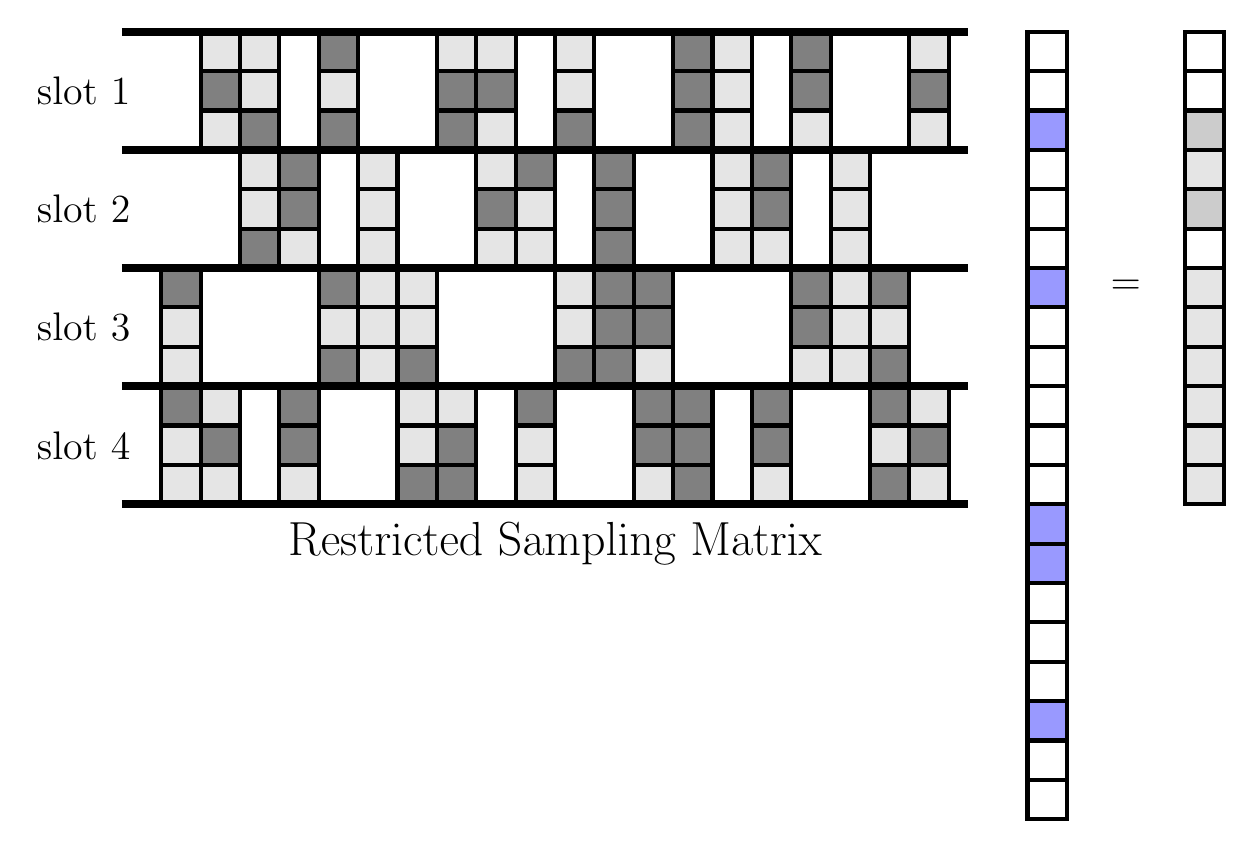
\begin{tikzpicture}
[draw=black, line width=1.5pt, >=stealth',
entry1/.style={rectangle, draw, fill=gray, inner sep=0pt, minimum size=5mm},
entry0/.style={rectangle, draw, fill=gray!20, inner sep=0pt, minimum size=5mm},
symbol0/.style={rectangle, draw, fill=white, inner sep=0pt, minimum size=5mm},
symbol/.style={rectangle, draw, fill=blue!40, inner sep=0pt, minimum size=5mm}]

\node[entry0] (m00) at (0,0) {};
\node[entry0] (m01) at (0.5,0) {};
%\node[entry1] (m02) at (1,0) {};
\node[entry0] (m03) at (1.5,0) {};
%\node[entry1] (m04) at (2,0) {};
%\node[entry0] (m05) at (2.5,0) {};
\node[entry1] (m06) at (3,0) {};
\node[entry1] (m07) at (3.5,0) {};
%\node[entry0] (m08) at (4,0) {};
\node[entry0] (m09) at (4.5,0) {};
%\node[entry1] (n00) at (5,0) {};
%\node[entry1] (n01) at (5.5,0) {};
\node[entry0] (n02) at (6,0) {};
\node[entry1] (n03) at (6.5,0) {};
%\node[entry0] (n04) at (7,0) {};
\node[entry0] (n05) at (7.5,0) {};
%\node[entry0] (n06) at (8,0) {};
%\node[entry0] (n07) at (8.5,0) {};
\node[entry1] (n08) at (9,0) {};
\node[entry0] (n09) at (9.5,0) {};


\node[entry0] (m10) at (0,0.5) {};
\node[entry1] (m11) at (0.5,0.5) {};
%\node[entry0] (m12) at (1,0.5) {};
\node[entry1] (m13) at (1.5,0.5) {};
%\node[entry0] (m14) at (2,0.5) {};
%\node[entry0] (m15) at (2.5,0.5) {};
\node[entry0] (m16) at (3,0.5) {};
\node[entry1] (m17) at (3.5,0.5) {};
%\node[entry1] (m18) at (4,0.5) {};
\node[entry0] (m19) at (4.5,0.5) {};
%\node[entry0] (n00) at (5,0.5) {};
%\node[entry1] (n11) at (5.5,0.5) {};
\node[entry1] (n12) at (6,0.5) {};
\node[entry1] (n13) at (6.5,0.5) {};
%\node[entry0] (n14) at (7,0.5) {};
\node[entry1] (n15) at (7.5,0.5) {};
%\node[entry1] (n16) at (8,0.5) {};
%\node[entry0] (n17) at (8.5,0.5) {};
\node[entry0] (n18) at (9,0.5) {};
\node[entry1] (n19) at (9.5,0.5) {};


\node[entry1] (m20) at (0,1) {};
\node[entry0] (m21) at (0.5,1) {};
%\node[entry0] (m22) at (1,1) {};
\node[entry1] (m23) at (1.5,1) {};
%\node[entry1] (m24) at (2,1) {};
%\node[entry0] (m25) at (2.5,1) {};
\node[entry0] (m26) at (3,1) {};
\node[entry0] (m27) at (3.5,1) {};
%\node[entry0] (m28) at (4,1) {};
\node[entry1] (m29) at (4.5,1) {};
%\node[entry0] (n20) at (5,1) {};
%\node[entry1] (n21) at (5.5,1) {};
\node[entry1] (n22) at (6,1) {};
\node[entry1] (n23) at (6.5,1) {};
%\node[entry0] (n24) at (7,1) {};
\node[entry1] (n25) at (7.5,1) {};
%\node[entry1] (n26) at (8,1) {};
%\node[entry0] (n27) at (8.5,1) {};
\node[entry1] (n28) at (9,1) {};
\node[entry0] (n29) at (9.5,1) {};


\node[entry0] (m30) at (0,1.5) {};
%\node[entry0] (m31) at (0.5,1.5) {};
%\node[entry1] (m32) at (1,1.5) {};
%\node[entry0] (m33) at (1.5,1.5) {};
\node[entry1] (m34) at (2,1.5) {};
\node[entry0] (m35) at (2.5,1.5) {};
\node[entry1] (m36) at (3,1.5) {};
%\node[entry1] (m37) at (3.5,1.5) {};
%\node[entry0] (m38) at (4,1.5) {};
%\node[entry0] (m39) at (4.5,1.5) {};
\node[entry1] (n30) at (5,1.5) {};
\node[entry1] (n31) at (5.5,1.5) {};
\node[entry0] (n32) at (6,1.5) {};
%\node[entry1] (n33) at (6.5,1.5) {};
%\node[entry0] (n34) at (7,1.5) {};
%\node[entry0] (n35) at (7.5,1.5) {};
\node[entry0] (n36) at (8,1.5) {};
\node[entry0] (n37) at (8.5,1.5) {};
\node[entry1] (n38) at (9,1.5) {};
%\node[entry0] (n39) at (9.5,1.5) {};


\node[entry0] (m40) at (0,2) {};
%\node[entry1] (m41) at (0.5,2) {};
%\node[entry0] (m42) at (1,2) {};
%\node[entry1] (m43) at (1.5,2) {};
\node[entry0] (m44) at (2,2) {};
\node[entry0] (m45) at (2.5,2) {};
\node[entry0] (m46) at (3,2) {};
%\node[entry1] (m47) at (3.5,2) {};
%\node[entry1] (m48) at (4,2) {};
%\node[entry0] (m49) at (4.5,2) {};
\node[entry0] (n40) at (5,2) {};
\node[entry1] (n41) at (5.5,2) {};
\node[entry1] (n42) at (6,2) {};
%\node[entry1] (n43) at (6.5,2) {};
%\node[entry0] (n44) at (7,2) {};
%\node[entry1] (n45) at (7.5,2) {};
\node[entry1] (n46) at (8,2) {};
\node[entry0] (n47) at (8.5,2) {};
\node[entry0] (n48) at (9,2) {};
%\node[entry1] (n49) at (9.5,2) {};


\node[entry1] (m50) at (0,2.5) {};
%\node[entry0] (m51) at (0.5,2.5) {};
%\node[entry0] (m52) at (1,2.5) {};
%\node[entry1] (m53) at (1.5,2.5) {};
\node[entry1] (m54) at (2,2.5) {};
\node[entry0] (m55) at (2.5,2.5) {};
\node[entry0] (m56) at (3,2.5) {};
%\node[entry0] (m57) at (3.5,2.5) {};
%\node[entry0] (m58) at (4,2.5) {};
%\node[entry1] (m59) at (4.5,2.5) {};
\node[entry0] (n50) at (5,2.5) {};
\node[entry1] (n51) at (5.5,2.5) {};
\node[entry1] (n52) at (6,2.5) {};
%\node[entry1] (n53) at (6.5,2.5) {};
%\node[entry0] (n54) at (7,2.5) {};
%\node[entry1] (n55) at (7.5,2.5) {};
\node[entry1] (n56) at (8,2.5) {};
\node[entry0] (n57) at (8.5,2.5) {};
\node[entry1] (n58) at (9,2.5) {};
%\node[entry0] (n59) at (9.5,2.5) {};


%\node[entry0] (m60) at (0,3) {};
%\node[entry0] (m61) at (0.5,3) {};
\node[entry1] (m62) at (1,3) {};
\node[entry0] (m63) at (1.5,3) {};
%\node[entry1] (m64) at (2,3) {};
\node[entry0] (m65) at (2.5,3) {};
%\node[entry1] (m66) at (3,3) {};
%\node[entry1] (m67) at (3.5,3) {};
\node[entry0] (m68) at (4,3) {};
\node[entry0] (m69) at (4.5,3) {};
%\node[entry1] (n60) at (5,3) {};
\node[entry1] (n61) at (5.5,3) {};
%\node[entry0] (n62) at (6,3) {};
%\node[entry1] (n63) at (6.5,3) {};
\node[entry0] (n64) at (7,3) {};
\node[entry0] (n65) at (7.5,3) {};
%\node[entry0] (n66) at (8,3) {};
\node[entry0] (n67) at (8.5,3) {};
%\node[entry1] (n68) at (9,3) {};
%\node[entry0] (n69) at (9.5,3) {};


%\node[entry0] (m70) at (0,3.5) {};
%\node[entry1] (m71) at (0.5,3.5) {};
\node[entry0] (m72) at (1,3.5) {};
\node[entry1] (m73) at (1.5,3.5) {};
%\node[entry0] (m74) at (2,3.5) {};
\node[entry0] (m75) at (2.5,3.5) {};
%\node[entry0] (m76) at (3,3.5) {};
%\node[entry1] (m77) at (3.5,3.5) {};
\node[entry1] (m78) at (4,3.5) {};
\node[entry0] (m79) at (4.5,3.5) {};
%\node[entry0] (n70) at (5,3.5) {};
\node[entry1] (n71) at (5.5,3.5) {};
%\node[entry1] (n72) at (6,3.5) {};
%\node[entry1] (n73) at (6.5,3.5) {};
\node[entry0] (n74) at (7,3.5) {};
\node[entry1] (n75) at (7.5,3.5) {};
%\node[entry1] (n76) at (8,3.5) {};
\node[entry0] (n77) at (8.5,3.5) {};
%\node[entry1] (n78) at (9,3.5) {};
%\node[entry1] (n79) at (9.5,3.5) {};


%\node[entry1] (m80) at (0,4) {};
%\node[entry0] (m81) at (0.5,4) {};
\node[entry0] (m82) at (1,4) {};
\node[entry1] (m83) at (1.5,4) {};
%\node[entry1] (m84) at (2,4) {};
\node[entry0] (m85) at (2.5,4) {};
%\node[entry0] (m86) at (3,4) {};
%\node[entry0] (m87) at (3.5,4) {};
\node[entry0] (m88) at (4,4) {};
\node[entry1] (m89) at (4.5,4) {};
%\node[entry0] (n80) at (5,4) {};
\node[entry1] (n81) at (5.5,4) {};
%\node[entry1] (n82) at (6,4) {};
%\node[entry1] (n83) at (6.5,4) {};
\node[entry0] (n84) at (7,4) {};
\node[entry1] (n85) at (7.5,4) {};
%\node[entry1] (n86) at (8,4) {};
\node[entry0] (n87) at (8.5,4) {};
%\node[entry1] (n88) at (9,4) {};
%\node[entry0] (n89) at (9.5,4) {};


%\node[entry0] (m90) at (0,4.5) {};
\node[entry0] (m91) at (0.5,4.5) {};
\node[entry1] (m92) at (1,4.5) {};
%\node[entry0] (m93) at (1.5,4.5) {};
\node[entry1] (m94) at (2,4.5) {};
%\node[entry0] (m95) at (2.5,4.5) {};
%\node[entry1] (m96) at (3,4.5) {};
\node[entry1] (m97) at (3.5,4.5) {};
\node[entry0] (m98) at (4,4.5) {};
%\node[entry0] (m99) at (4.5,4.5) {};
\node[entry1] (n90) at (5,4.5) {};
%\node[entry1] (n91) at (5.5,4.5) {};
%\node[entry0] (n92) at (6,4.5) {};
\node[entry1] (n93) at (6.5,4.5) {};
\node[entry0] (n94) at (7,4.5) {};
%\node[entry0] (n95) at (7.5,4.5) {};
\node[entry0] (n96) at (8,4.5) {};
%\node[entry0] (n97) at (8.5,4.5) {};
%\node[entry1] (n98) at (9,4.5) {};
\node[entry0] (n99) at (9.5,4.5) {};


%\node[entry0] (m100) at (0,5) {};
\node[entry1] (m101) at (0.5,5) {};
\node[entry0] (m102) at (1,5) {};
%\node[entry1] (m103) at (1.5,5) {};
\node[entry0] (m104) at (2,5) {};
%\node[entry0] (m105) at (2.5,5) {};
%\node[entry0] (m106) at (3,5) {};
\node[entry1] (m107) at (3.5,5) {};
\node[entry1] (m108) at (4,5) {};
%\node[entry0] (m109) at (4.5,5) {};
\node[entry0] (n100) at (5,5) {};
%\node[entry1] (n101) at (5.5,5) {};
%\node[entry1] (n102) at (6,5) {};
\node[entry1] (n103) at (6.5,5) {};
\node[entry0] (n104) at (7,5) {};
%\node[entry1] (n105) at (7.5,5) {};
\node[entry1] (n106) at (8,5) {};
%\node[entry0] (n107) at (8.5,5) {};
%\node[entry0] (n108) at (9,5) {};
\node[entry1] (n109) at (9.5,5) {};


%\node[entry1] (m110) at (0,5.5) {};
\node[entry0] (m111) at (0.5,5.5) {};
\node[entry0] (m112) at (1,5.5) {};
%\node[entry1] (m113) at (1.5,5.5) {};
\node[entry1] (m114) at (2,5.5) {};
%\node[entry0] (m115) at (2.5,5.5) {};
%\node[entry0] (m116) at (3,5.5) {};
\node[entry0] (m117) at (3.5,5.5) {};
\node[entry0] (m118) at (4,5.5) {};
%\node[entry1] (m119) at (4.5,5.5) {};
\node[entry0] (n110) at (5,5.5) {};
%\node[entry1] (n111) at (5.5,5.5) {};
%\node[entry1] (n112) at (6,5.5) {};
\node[entry1] (n113) at (6.5,5.5) {};
\node[entry0] (n114) at (7,5.5) {};
%\node[entry1] (n115) at (7.5,5.5) {};
\node[entry1] (n116) at (8,5.5) {};
%\node[entry0] (n117) at (8.5,5.5) {};
%\node[entry1] (n118) at (9,5.5) {};
\node[entry0] (n119) at (9.5,5.5) {};

  \foreach \line in {0,1,2,3,4} {
    \draw[line width=3] (-0.75, -0.25+1.5*\line) -- (10,-0.25+1.5*\line);
  }
  \foreach \line in {1,2,3,4} {
    \node[anchor=east] (slot\line) at (-0.5,6.5-1.5*\line) {\Large slot \line};
  }


\node[symbol0] (s1) at (11,-4) {};
\node[symbol0] (s2) at (11,-3.5) {};
\node[symbol] (s3) at (11,-3) {};
\node[symbol0] (s4) at (11,-2.5) {};
\node[symbol0] (s5) at (11,-2) {};
\node[symbol0] (s6) at (11,-1.5) {};
\node[symbol] (s7) at (11,-1) {};
\node[symbol] (s8) at (11,-0.5) {};
\node[symbol0] (s9) at (11,0) {};
\node[symbol0] (s10) at (11,0.5) {};
\node[symbol0] (s11) at (11,1) {};
\node[symbol0] (s12) at (11,1.5) {};
\node[symbol0] (s13) at (11,2) {};
\node[symbol] (s14) at (11,2.5) {};
\node[symbol0] (s15) at (11,3) {};
\node[symbol0] (s16) at (11,3.5) {};
\node[symbol0] (s17) at (11,4) {};
\node[symbol] (s18) at (11,4.5) {};
\node[symbol0] (s19) at (11,5) {};
\node[symbol0] (s20) at (11,5.5) {};

\node (equal) at (12,2.5) {\Large =};

\node[entry0,fill=black!10] (y0) at (13,0) {};
\node[entry0,fill=black!10] (y1) at (13,0.5) {};
\node[entry0,fill=black!10] (y2) at (13,1) {};
\node[entry0,fill=black!10] (y3) at (13,1.5) {};
\node[entry0,fill=black!10] (y4) at (13,2) {};
\node[entry0,fill=black!10] (y5) at (13,2.5) {};
\node[entry0,fill=black!00] (y6) at (13,3) {};
\node[entry0,fill=black!20] (y7) at (13,3.5) {};
\node[entry0,fill=black!10] (y8) at (13,4) {};
\node[entry0,fill=black!20] (y9) at (13,4.5) {};
\node[entry0,fill=black!00] (y10) at (13,5) {};
\node[entry0,fill=black!00] (y11) at (13,5.5) {};


\node (samplingmatrix) at (4.75,-0.75) {\LARGE Restricted Sampling Matrix};

\end{tikzpicture}

}
\end{center}
\begin{columns}
\column{.45\textwidth}
\begin{itemize}
\item Partition into $V$ slot
\item $\tilde{N} = N/V$ channel uses
\end{itemize}
\column{.5\textwidth}
\begin{itemize}
\item Aim is $T$-user adder channel
%\begin{equation*}
%\tilde{y}_j = \sum_{i \in \mathcal{N}_j} \tilde{x}_{w_i} + \tilde{z}_j,
%\end{equation*}
%where $\mathcal{N}_j$ is active users in slot~$j$
\item Admits graphical representation
\end{itemize}
\end{columns}
\end{frame}


\begin{frame}
\frametitle{Unsourced MAC -- Low Complexity State-of-the-Art}
\begin{center}
\scalebox{0.75}{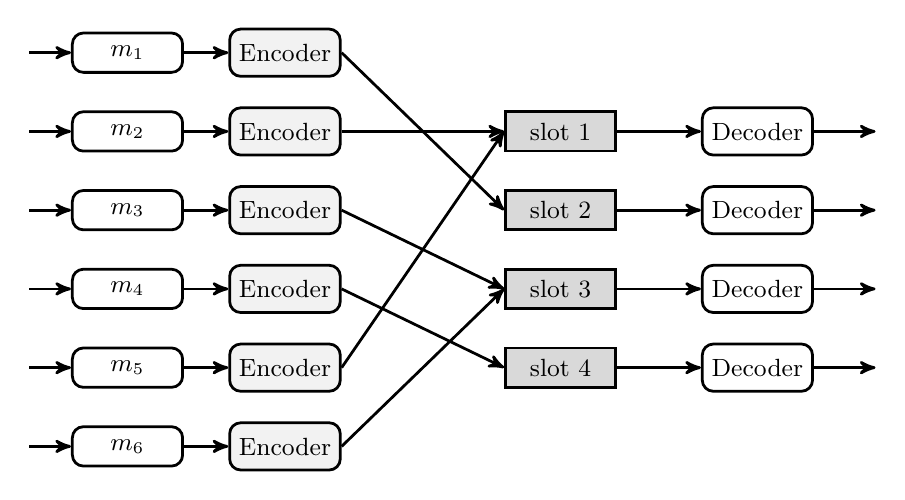
\begin{tikzpicture}
  [
  font=\small, line width=1pt, draw=black, >=stealth',
  slot/.style={rectangle, minimum height=5mm, minimum width=14mm, draw=black, fill=gray!30},
  encoder/.style={rectangle, minimum height=6mm, minimum width=14mm, draw=black, fill=gray!10, rounded corners},
  decoder/.style={rectangle, minimum height=6mm, minimum width=14mm, draw=black, rounded corners},
  message/.style={rectangle, minimum height=5mm, minimum width=14mm, draw=black, rounded corners}
  ]

\foreach \e in {1,2,3,4,5,6} {
  \node[encoder] (e\e) at (2,0.5-\e) {Encoder};
}

\foreach \m in {1,2,3,4,5,6} {
  \node[message] (m\m) at (0,0.5-\m) {$m_{\m}$}
  edge[->] (e\m);
  \draw[<-] (m\m) -- (-1.25,0.5-\m);
}
  
\foreach \s in {1,2,3,4} {
  \node[slot] (c\s) at (5.5,-0.5-\s) {slot~\s};
  \node[decoder] (d\s) at (8,-0.5-\s) {Decoder};
  \draw[->] (c\s) -- (d\s);
}

\draw[->] (d1.east) -- (9.5,-1.5);
\draw[->] (d2.east) -- (9.5,-2.5);
\draw[->] (d3.east) -- (9.5,-3.5);
\draw[->] (d4.east) -- (9.5,-4.5);

\draw[->] (e1.east) -- (c2.west);
\draw[->] (e2.east) -- (c1.west);
\draw[->] (e3.east) -- (c3.west);
\draw[->] (e4.east) -- (c4.west);
\draw[->] (e5.east) -- (c1.west);
\draw[->] (e6.east) -- (c3.west);
\end{tikzpicture}

}
\end{center}
\begin{itemize}
\item Every active devices randomly select one sub-block
\item Inner code designed to recover modulo-$p$ sum of codewords
\item Outer code is designed to decode multiple messages given the modulo-$p$ sum of their codewords
%\item Scheme uses large number of slots to ensure that every message is received in slot containing fewer than $T$ messages.
\end{itemize}
\footnotetext[1]{
O. Ordentlich and Y. Polyanskiy. ``Low Complexity Schemes for the Random Access Gaussian Channel.'' ISIT, 2017.}
\end{frame}


\begin{frame}
\frametitle{Unsourced MAC -- Proposed Scheme}
\begin{center}
\scalebox{0.75}{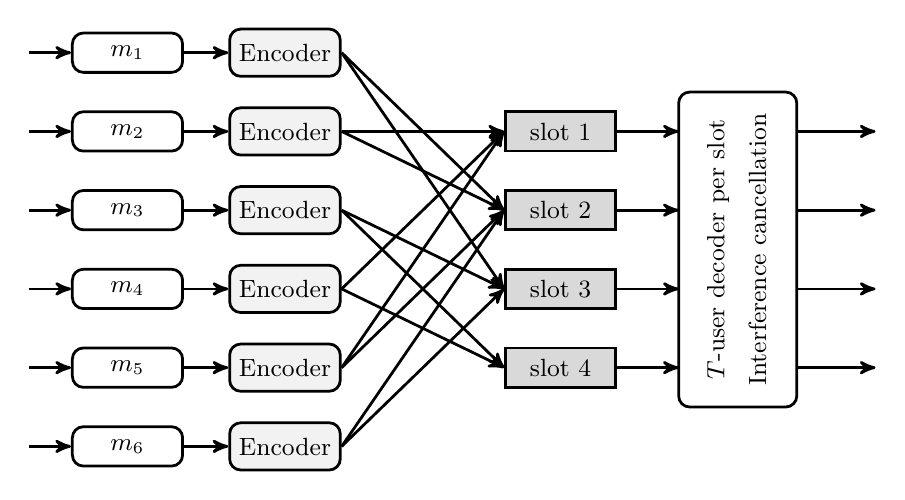
\begin{tikzpicture}
  [
  font=\small, line width=1pt, draw=black, >=stealth',
  slot/.style={rectangle, minimum height=5mm, minimum width=14mm, draw=black, fill=gray!30},
  encoder/.style={rectangle, minimum height=6mm, minimum width=14mm, draw=black, fill=gray!10, rounded corners},
  decoder/.style={rectangle, minimum height=6mm, minimum width=14mm, draw=black, rounded corners},
  message/.style={rectangle, minimum height=5mm, minimum width=14mm, draw=black, rounded corners}
  ]

\foreach \e in {1,2,3,4,5,6} {
  \node[encoder] (e\e) at (2,0.5-\e) {Encoder};
}

\foreach \m in {1,2,3,4,5,6} {
  \node[message] (m\m) at (0,0.5-\m) {$m_{\m}$}
  edge[->] (e\m);
  \draw[<-] (m\m) -- (-1.25,0.5-\m);
}
  
\foreach \s in {1,2,3,4} {
  \node[slot] (c\s) at (5.5,-0.5-\s) {slot~\s};
  %\node[decoder] (d\s) at (8,-0.5-\s) {Decoder};
  \draw[->] (c\s) -- (7,-0.5-\s);
}

\draw[rounded corners] (7,-1) rectangle (8.5,-5);
\node[rotate=90] (d1) at (7.5,-3) {$T$-user decoder per slot};
\node[rotate=90] (d2) at (8,-3) {Interference cancellation};

\draw[->] (8.5,-1.5) -- (9.5,-1.5);
\draw[->] (8.5,-2.5) -- (9.5,-2.5);
\draw[->] (8.5,-3.5) -- (9.5,-3.5);
\draw[->] (8.5,-4.5) -- (9.5,-4.5);

\draw[->] (e1.east) -- (c2.west);
\draw[->] (e2.east) -- (c1.west);
\draw[->] (e3.east) -- (c3.west);
\draw[->] (e4.east) -- (c4.west);
\draw[->] (e5.east) -- (c1.west);
\draw[->] (e6.east) -- (c3.west);
\draw[->] (e1.east) -- (c3.west);
\draw[->] (e2.east) -- (c2.west);
\draw[->] (e3.east) -- (c4.west);
\draw[->] (e4.east) -- (c1.west);
\draw[->] (e5.east) -- (c2.west);
\draw[->] (e6.east) -- (c2.west);
\end{tikzpicture}
}
\end{center}
\begin{itemize}
\item Schedule selected based on \textbf{message}
\item Devices can transmit in multiple sub-blocks
\item Scheme facilitates successive interference cancelation
\end{itemize}
\footnotetext[1]{
A. Vem, K. Narayanan, J. Cheng, J.-F. Chamberland}
\end{frame}


\begin{frame}
\frametitle{What Really Happens within Slot?}
\begin{center}
\scalebox{1}{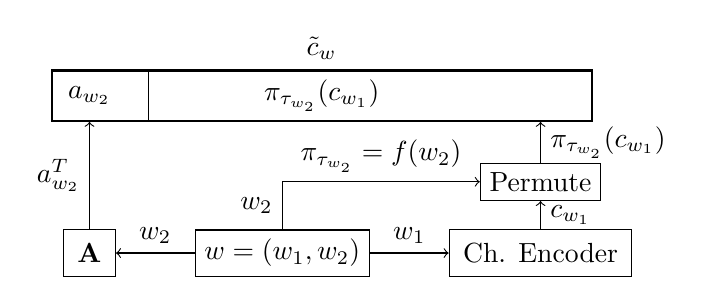
\begin{tikzpicture}

%Message node and final codeword Rectangle
\node[draw,rectangle] (msg) at (3,1) {$w=(w_1,w_2)$};
\node[rectangle, draw, minimum width=2.7in,thick] (codeword) at (3.5,3) {$\pi_{\tau_{w_2}}({c}_{w_1})$}; 
%$c_{w}(\pi_{\tau_{w_2}^1}),c_{w}(\pi_{\tau_{w_2}^2}),\ldots,c_{w}(\pi_{\tau_{w_2}})$};


% From messages to Ch. Encoder and Compressive Sensing Encoder
\draw [->] (msg.east) -- +(0:1) node[midway, above] {$w_1$} node[draw, inner sep=5pt,at end, anchor= west] (encoder) {Ch. Encoder} ;
\draw [->] (msg.west) -- +(0:-1) node[midway, above] {$w_2$} node[draw, inner sep=5pt,at end, anchor= east] (CSencoder) {$\mathbf{A}$}; %{Sensing Matrix $\mathbf{A}$};

\path (encoder.north)-- +(90:0.6) node[draw, rectangle,fill=white](CWperm){Permute};
\draw[->] (encoder.north)-- (CWperm.south) node[midway,right]{${c}_{w_1}$};
\draw[->](CWperm.north)-- (CWperm.north |- codeword.south) node[midway, right]{$\pi_{\tau_{w_2}}({c}_{w_1})$};

\draw[->](CSencoder.north)-- (CSencoder.north |- codeword.south) node[midway, left]{${a}^T_{w_2}$};

\path let \p{A}=(codeword) in (3-1.7,\y{A})node (partition){} -- (partition |- codeword.north);
\draw (partition |- codeword.north) -- (partition |- codeword.south) ;
\node () at (partition -| CSencoder) {${a}_{w_2}$};
\node [above] at (codeword.north) {${\tilde{c}}_{w}$};

\draw [->] (msg.north) -- (msg.north |- CWperm.west)node[midway,left]{$w_2$} -- (CWperm.west) node[midway,above] {$\pi_{\tau_{w_2}}=f(w_2)$};
\end{tikzpicture}
}
\end{center}
\begin{itemize}
\item Message is partitioned into two parts $w = (w_1, w_2)$
\item Every device uses identical codebook built from LDPC-type codes tailored to $T$-user real-adder channel
\item $w_2$ dictate permutation on encoder and recovered through CS
\item Non-negative $\ell_1$-regularized LASSO
\item Spatially-coupled low-density parity check code is employed
%\item MMSE estimator on list
\end{itemize}
\footnotetext[1]{
A. Vem, K. Narayanan, J. Cheng, J.-F. Chamberland}
\end{frame}


\begin{frame}
\frametitle{What Really Happens within Slot?}
\begin{center}
\scalebox{0.5}{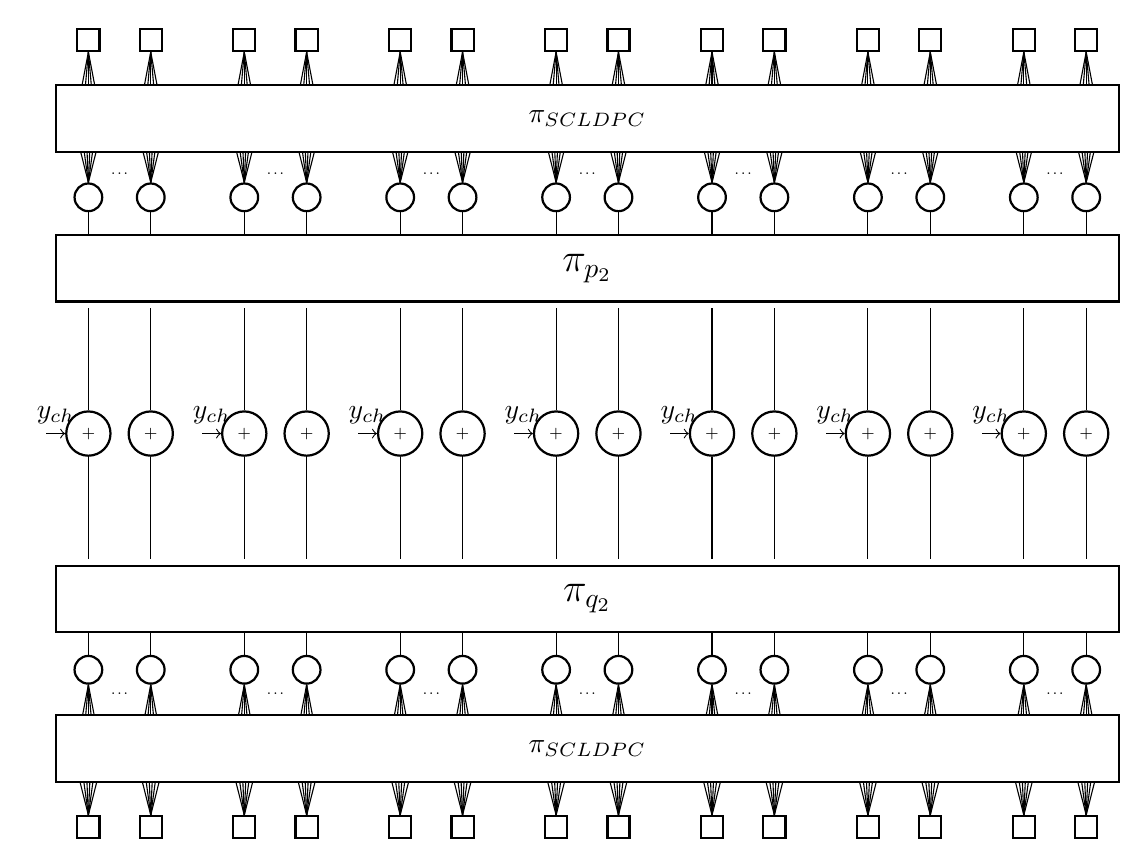
\begin{tikzpicture}[
  xscale=0.33,yscale=1,
  bitnode/.style={circle,minimum size=10pt,thick,draw=black,fill=white},
  bitnodeblack/.style={circle,minimum size=10pt,thick,draw=black,fill=white},
  bitnodewhite/.style={circle,minimum size=10pt,thick,draw=white,fill=gray},
  bitnode2/.style={circle,minimum size=10pt,thick,draw=black,fill=gray},
  bitnode2black/.style={circle,minimum size=10pt,thick,draw=black,fill=gray},
  bitnode2white/.style={circle,minimum size=10pt,thick,draw=white,fill=white},
  checknode/.style={rectangle,minimum size=8pt,thick,draw=black,fill=white},
  checknodeblack/.style={rectangle,minimum size=8pt,thick,draw=black,fill=white},
  checknodewhite/.style={rectangle,minimum size=8pt,thick,draw=white,fill=white},
  permnode/.style={rectangle,very thin,minimum width=30pt,minimum height=18pt,fill=white,draw=black},
  permnodeblack/.style={rectangle,very thin,minimum width=30pt,minimum height=18pt,fill=white,draw=black},
  permnodewhite/.style={rectangle,very thin,minimum width=30pt,minimum height=18pt,fill=white,draw=white},
  permedge/.style={black!65},
  permedgeblack/.style={black!65},
  permedgewhite/.style={white},
  ]

  \def \cndist {1.2}
  \def \vndist {1.2}
  \def \ccndist {1.2}
  \def \vvny {2.75}
  \def \cny {3}
  \def \vny {1}
  \def \vnya {-2}
  \def \vnyb {-5}
  \def \ccny {-7}
    \def \ext{1.3}
      \def \exta {1}
  \def \midx   {0.5}
  
    \tikzstyle{bigPerm}= [rectangle, draw, thick, minimum width=320*\vndist, minimum height=20*\vndist,fill=white, draw=black]
    
\def\ldgcol{black}
\def\ldpcol{black}
\def\seqa{black}
\def\seqb{black}
    \foreach \x/\i in {0/1,6/2,12/3,18/4,24/5,30/6,36/7} {

      \node[bitnode\seqa] (v1\i) at (\x-\vndist, \vny) {};
      \node[bitnode\seqa] (v2\i) at (\x+\vndist, \vny) {};
      \node at (\x,\vny+0.3) {\tiny{$...$}};
% Edges- LDPC bits to top
      \draw[\seqa] (v1\i.north) -- +(52.5:1);
      \draw[\seqa] (v1\i.north) -- +(67.5:1);
      \draw[\seqa] (v1\i.north) -- +(82.5:1);
      \draw[\seqa] (v1\i.north) -- +(97.5:1);
      \draw[\seqa] (v1\i.north) -- +(112.5:1);
      \draw[\seqa] (v1\i.north) -- +(127.5:1);

      \draw[\seqa] (v2\i.north) -- +(52.5:1);
      \draw[\seqa] (v2\i.north) -- +(67.5:1);
      \draw[\seqa] (v2\i.north) -- +(82.5:1);
      \draw[\seqa] (v2\i.north) -- +(97.5:1);
      \draw[\seqa] (v2\i.north) -- +(112.5:1);
      \draw[\seqa] (v2\i.north) -- +(127.5:1);


     \node[bitnode\seqb] (v3\i) at (\x-\vndist, \vnyb) {};
     \node[bitnode\seqb] (v4\i) at (\x+\vndist, \vnyb) {};
     \node at (\x,\vnyb-0.3) {\tiny{$...$}};
     
% Edges- LDPC bits to bottom
      \draw[\seqb] (v3\i.south) -- +(240:1);
      \draw[\seqb] (v3\i.south) -- +(255:1);
      \draw[\seqb] (v3\i.south) -- +(270:1);
      \draw[\seqb] (v3\i.south) -- +(285:1);
      \draw[\seqb] (v3\i.south) -- +(300:1);

      \draw[\seqb] (v4\i.south) -- +(240:1);
      \draw[\seqb] (v4\i.south) -- +(255:1);
      \draw[\seqb] (v4\i.south) -- +(270:1);
      \draw[\seqb] (v4\i.south) -- +(285:1);
      \draw[\seqb] (v4\i.south) -- +(300:1);

% Middle bits= Actual GMAC Code bits
    \node[bitnode] (v5\i) at (\x-\vndist, \vnya) {\tiny $+$};
    \node[bitnode] (v6\i) at (\x+\vndist, \vnya) {\tiny $+$};
     

    \draw (v1\i.south) -- +(270:\exta);      \draw (v2\i.south) -- +(270:\exta);    
    \draw (v3\i.north) -- +(90:\exta);        \draw (v4\i.north) -- +(90:\exta);

    \draw (v5\i.north)-- +(90:\ext);       \draw (v6\i.north)-- +(90:\ext);
    \draw (v5\i.south) -- +(270:\ext);    \draw (v6\i.south) -- +(270:\ext);

    \draw[<-] (v5\i.west) -- node[midway, above]{$y_{\text{ch}}$} +(-0.6*\vndist,0);

% Top Checks
 \node[checknode\ldgcol] (c1\i) at (\x-\cndist, \cny) {};
  \node[checknode\ldgcol] (c2\i) at (\x+\cndist, \cny) {};

% Top check to bottom
      \draw[\ldgcol] (c1\i.south) -- +(240:1);
      \draw[\ldgcol] (c1\i.south) -- +(255:1);
      \draw[\ldgcol] (c1\i.south) -- +(270:1);
      \draw[\ldgcol] (c1\i.south) -- +(285:1);
      \draw[\ldgcol] (c1\i.south) -- +(300:1);

      \draw[\ldgcol] (c2\i.south) -- +(240:1);
      \draw[\ldgcol] (c2\i.south) -- +(255:1);
      \draw[\ldgcol] (c2\i.south) -- +(270:1);
      \draw[\ldgcol] (c2\i.south) -- +(285:1);
      \draw[\ldgcol] (c2\i.south) -- +(300:1);

  
%Bottom Checks  
      \node[checknode\ldpcol] (cc1\i) at (\x-\ccndist, \ccny) {};
      \node[checknode\ldpcol] (cc2\i) at (\x+\ccndist, \ccny) {};
      
% Bottom checks to top
      \draw[\ldpcol] (cc1\i.north) -- +(52.5:1);
      \draw[\ldpcol] (cc1\i.north) -- +(67.5:1);
      \draw[\ldpcol] (cc1\i.north) -- +(82.5:1);
      \draw[\ldpcol] (cc1\i.north) -- +(97.5:1);
      \draw[\ldpcol] (cc1\i.north) -- +(112.5:1);
      \draw[\ldpcol] (cc1\i.north) -- +(127.5:1);

      \draw[\ldpcol] (cc2\i.north) -- +(52.5:1);
      \draw[\ldpcol] (cc2\i.north) -- +(67.5:1);
      \draw[\ldpcol] (cc2\i.north) -- +(82.5:1);
      \draw[\ldpcol] (cc2\i.north) -- +(97.5:1);
      \draw[\ldpcol] (cc2\i.north) -- +(112.5:1);
      \draw[\ldpcol] (cc2\i.north) -- +(127.5:1);

      \node[\ldpcol] at (\x,-5.7) {\tiny{$...$}};
      \node[\ldgcol] at (\x,1.7) {\tiny{$...$}};

}

  \node[bigPerm] (perm1_node) at (18,0.5*\vny+0.5*\cny) {\normalsize $\pi_{\text{SCLDPC}}$};    
  \node[bigPerm] (perm2_node) at (18,0.5*\vnyb+0.5*\ccny) {\normalsize $\pi_{\text{SCLDPC}}$};    
  
  \node[bigPerm] (perm3_node) at (18,0.7*\vny+0.3*\vnya) {\Large $\pi_{p_2}$};    
  \node[bigPerm] (perm4_node) at (18,0.3*\vnya+0.7*\vnyb) {\Large $\pi_{q_2}$};    
   
\end{tikzpicture}}
\end{center}
\begin{itemize}
\item Run joint belief propagation (BP) decoder
\end{itemize}
\footnotetext[1]{
A. Vem, K. Narayanan, J. Cheng, J.-F. Chamberland}
\end{frame}


\begin{frame}
\frametitle{Side by Side}
\begin{center}
\scalebox{0.5}{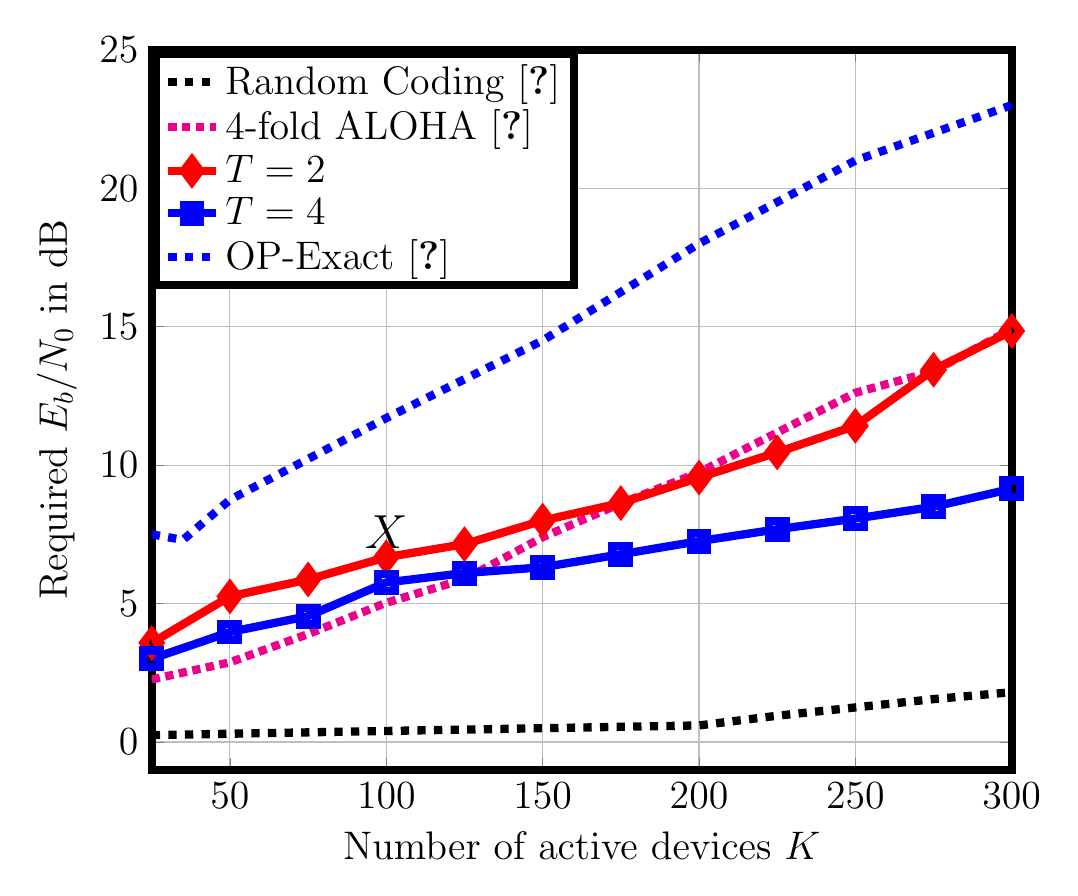
\begin{tikzpicture}
% The SC paramaters for the below set of plots are
% L=16
% w=3.
% So the true rate R is related to design rate R'(=1-dc/dv) as
% 1-R=(L+w-1)*(1-R')/L
\def\fsize{\large}
%\pgfplotsset{every y tick label/.append style={font=\fsize}}
%\pgfplotsset{every x tick label/.append style={font=\fsize}}

\begin{axis}[%
font=\Large,
width=4.3in,
height=3.6in,
scale only axis,
xmin=25,
xmax=300,
xtick = {50,100,...,300},
xlabel={{Number of active devices $K$}},
ylabel={{Required $E_b / N_0$ in dB}},
xmajorgrids,
xminorgrids,
ymin=-1,
ymax=25,
ytick = {-5,0,...,30},
yminorticks=true,
ymajorgrids,
yminorgrids,
line width=3.0pt,
legend style={at={(0,1)},anchor=north west, draw=black,fill=white,legend cell align=left}
]

\node[] at (axis cs: 100,7.5696) {\LARGE $X$};
%\addplot [color=red,solid,mark=asterisk,mark size=4.0]
%  table[row sep=crcr]{
%  25    5.4282    \\% 0.70   41   54  10  26    -4.6875
%  50    6.6231    \\%0.20   22   40   6  54    -6.0156
%  75    7.6800    \\%0.20   --   --   8  35    ----
%100   8.3966 \\ % 0.10   37   71   8  32    -2.5000
%125   9.3623  \\%0.10   46   88   8  29    -0.7812
%150  10.219 \\ %0.05   52  102  10  23     0.3125
%175  11.2638\\ %0.12   64  121   8  26     2.1875
%200  11.9196 \\%0.08   69  133  10  23     2.8516 %lambda=[0:0.04:0.2],alpha=[4:2:10]
%225  12.7696\\ %0.10   79  151   8  26     4.2188 %lambda=[0:0.02:0.16],alpha=[4:2:10]
%250  14.1942 \\%0.02   82  163   8  26     5.6250 %    """             ,alpha=[8:2:12]
%275  15.0855\\ %0.10   96  183   8  26     6.9531 %    """             ,alpha=[8:2:12]
%300  16.0261 \\%0.06  101  196   8  26     7.9297 %    """             ,alpha=[8:2:12]
%};
%\addlegendentry{T=2};
%

%\addplot [color=blue,solid,mark=square,mark size=4.0]%,mark options={solid}]
%  table[row sep=crcr]{
%  25  3.8366  \\%0.90   15   17   6  155  -10.2734
% 50  4.9716\\%  0.90   33   37   8   65   -5.9766
% 75  6.5251 \\% 0.40   17   28  10   65   -7.6953 alpha=6:2:12
%100  6.9418 \\% 0.40   23   37  12   47   -6.3281 alpha=6:2:12
%125  7.4985 \\% 0.30   24   41   8   65   -5.5469 alpha=8:2:14
%150  8.3487  \\%0.20   26   47  10   50   -4.5703 alpha=8:2:14
%175  8.8836  \\%0.35   36   60  14   32   -2.9102 alpha=8:2:14
%200  9.4339  \\%0.25   36   63  16   28   -2.5195 alpha=10:2:16; lambda=0.05:.05:0.35;
%225 10.1554 \\% 0.30   41   70  12   35   -1.2500 alpha=10:2:16; lambda=0.05:.05:0.45;
%250 10.9185  \\%0.30   45   77  12   35   -0.2734 alpha=10:2:16; lambda=0.05:.05:0.4;
%275 11.5795 \\% 0.25   48   84  18   24    0.3125 alpha= 12:2:18;lambda=0.05:.05:0.35;
%300 12.2223 \\% 0.25   51   90  18   24    1.0938 alpha= 12:2:18;lambda=0.05:.05:0.35;
%};
%\addlegendentry{T=4};


%\addplot [color=black,solid,mark=circle,mark options=solid,mark size=4.0]%,mark options={solid}]
%  table[row sep=crcr]{
%   25 4.1796 \\ %1.00  9  9  8 320 -13.2812 alpha=2:2:10,lambda=1:-0.1:0.7
% 50 4.9560 \\ %1.00 20 20 10 140  -9.4531 alpha=2:2:10,lambda=1:-0.1:0.7
% 75  5.6438 \\ %1.00 30 30  8 110  -6.8359 alpha=4:2:12,lambda=1:-0.1:0.7
%100  6.6047 \\ %1.00 42 42 10  73  -4.7656 alpha=4:2:12,lambda=1:-0.1:0.7
%150  7.7143 \\ %0.40 20 32 14  65  -6.8359 alpha=6:2:14,lambda=1:-0.1:0.2
%200  8.4836 \\ %0.40 26 42 18  43 -5.1562  alpha=10:2:18;lambda=0:0.1:0.4;
%250  9.4684 \\ %0.40 31 50 20  35 -3.5938  alpha=12:2:20;lambda=0:0.1:0.4;
%%300  11.251 \\ %0.40 40 64 18  35 -1.0547  alpha=12:2:20;lambda=0.2:0.1:0.6;
%300  11.1223 \\%0.35 36 60 16.0 43 -1.6406
%};
%\addlegendentry{T=6};


\addplot [color=black,solid,dashed]
  table[row sep=crcr]{
  25     0.25\\
 50     0.3\\
 75     0.35\\
100     0.4\\
125     0.45\\
150     0.5\\
175    0.55\\
200  0.60\\
225 0.95\\
250 1.25\\
275 1.55\\
300 1.8\\
};
\addlegendentry{Random Coding \cite{polyanskiy17}};



%\addplot [color=green,solid]
%  table[row sep=crcr]{
%  25   1.44  \\% 13
%  50   1.88  \\% 27
%  75   2.40  \\% 39
% 100   3.27 \\%  52
% 125   4.43 \\%  68
% 150   5.30 \\%  80
% 175   6.42 \\%  93
% 200   7.36\\%  106
% 225   8.39\\%  120
% 250   9.72 \\% 135
% 275  10.80 \\% 149
% 300  11.80 \\% 162
%};
%\addlegendentry{5-fold ALOHA};

\addplot [color=magenta,dotted]
  table[row sep=crcr]{
  25   2.26  \\
  50   2.88  \\
  75   3.90  \\
 100   5.03 \\
  125.0000    5.8798 \\
  150.0000    7.3954 \\
  175.0000    8.6199 \\
  200.0000    9.7328 \\
  225.0000   11.1761\\
  250.0000   12.6127\\
  275.0000   13.3907\\
  300.0000   14.9116\\
  };
\addlegendentry{4-fold ALOHA \cite{ordentlich17}};

\addplot [color=red,solid,mark=diamond,mark size=4.0]
  table[row sep=crcr]{
  25   3.5820  \\
  50   5.2585 \\
  75   5.8700  \\
100  6.6738 \\
125  7.1463 \\
150  7.9984 \\
175  8.63 \\
200  9.55 \\
225  10.46 \\
250  11.42 \\
275 13.4438 \\
300 14.8439 \\
};
\addlegendentry{$T=2$};

%\addplot [color=red,solid,mark=diamond,mark size=4.0]
%  table[row sep=crcr]{
%  25   2.1522  \\
%  50   4.0581\\
%  75   4.5625\\
%100  5.3325 \\
%125    5.4330\\
%150  5.8549 \\
%175  6.3787\\
%200  6.6580 \\
%225  7.9109\\
%250  8.5476\\
%275   9.5476\\
% 300 10.3177\\
%};
%\addlegendentry{T=2};


%\addplot [color=blue,solid,mark=square,mark size=3.0]
%  table[row sep=crcr]{
% 25 2.1178\\
% 50 2.6828\\
% 75 3.1482 \\
%100 3.7733\\
%125 4.6866\\
%150 5.4191\\
%175 5.4495\\
%200 5.6737\\
%225 6.0074\\
%250 6.0881\\
%275 6.9083\\
%300 6.8751\\
%};
%\addlegendentry{T=4};



\addplot [color=blue,solid,mark=square,mark size=3.0]
  table[row sep=crcr]{
  25   3.0077  \\
  50   3.9733 \\
  75   4.5465 \\
100   5.7622 \\
125  6.1017 \\
150  6.3117 \\
175  6.7814 \\
200  7.2532 \\
225  7.6838 \\
250  8.0691\\
275  8.4960 \\
300 9.1467 \\
};
\addlegendentry{$T=4$};


\addplot [color=blue,dashed]
  table[row sep=crcr]{
  25   7.50 \\
   35   7.30 \\
  50   8.75 \\
  100 11.7 \\
  150 14.50\\
%175  6.7814 \\
200  18\\
%225  7.6838 \\
250  21\\
%275  8.4960 \\
300 23\\
};
\addlegendentry{OP-Exact \cite{ordentlich17}};


\end{axis}
\end{tikzpicture}% 
}
\end{center}
\begin{itemize}
\item Minimum $E_b/N_0$ required as function of \# of devices
\item For $T=2,4$ and $4$-fold ALOHA, prob.\ of decoding every slot $\geq 0.99$
\item Prob.\ recovered messages $\geq 0.96$ given $T$-user decoding successful
\end{itemize}
\footnotetext[1]{
A. Vem, K. Narayanan, J. Cheng, J.-F. Chamberland}
\end{frame}


\begin{frame}
\frametitle{Discussion -- Unsourced Multiple Access}
\begin{itemize}
\item New framework for Unsourced Multiple Access
\item Leverages power and lessons from graphical model
\item Proposed scheme outperforms state-of-the-art
\begin{itemize}
\item Takes advantage of successive interference cancellation
\item Relax requirement for keeping maximum devices per slot below $T$
\item Takes advantage of $T$-user real-adder channel via BP
\end{itemize}
\item Complexity needs to be tracked better
\item Design of sampling matrix $A$ can be optimized
\end{itemize}
\end{frame}


\begin{frame}
\frametitle{Questions?}
\centerline{\Large Thank You}
\end{frame}


\end{document}
